% 第 2 章
\bichapter{准备设计}{Preparing the Design}
\label{chap:prep}

Fusion Compiler 工具使用设计库（design library）来存储设计及其相关库信息。本节说明如何创建设计库，以及如何准备并保存设计。

这些步骤在以下主题中说明：
\begin{itemize}
  \item 定义搜索路径（Defining the Search Path）
  \item 设置库（Setting Up Libraries）
  \item 使用 Pin Access Checker 实用程序
  \item 分析库（Analyzing Libraries）
  \item 读取设计（Reading the Design）
  \item 缓解设计不匹配（Mitigating Design Mismatches）
  \item 导入 floorplan 信息
  \item 设置多电压设计（Setting Up Multivoltage Designs）
  \item 指定时序约束与设置
  \item 指定逻辑设计规则约束
  \item 指定时钟门控约束（Specifying Clock Gating Constraints）
  \item 为布局与合法化指定物理约束
  \item 指定布局设置
  \item 指定合法化设置
  \item 控制单元、net、pin 与 port 的优化
  \item 指定布线前优化设置
  \item 为功耗相关功能做准备
  \item 指定布线资源
  \item 使用 Early Data Check Manager 处理设计数据
  \item 应用 Mega-Switch 命令设置
\end{itemize}

% ============================================================
\section{定义搜索路径}
\subsection*{Defining the Search Path}

Fusion Compiler 工具使用搜索路径（search path）查找以相对路径指定、或未指定路径的文件。

要用 \cmd{set\_app\_var} 命令将 \appopt{search\_path} 应用变量设为按顺序查找文件的目录列表。工具查找文件时，从 \appopt{search\_path} 中最左侧的目录开始，使用找到的第一个匹配文件。

也可用 Tcl 的 \cmd{lappend} 命令把目录追加到默认搜索路径（即启动工具时所在目录）。例如：
\begin{lstlisting}
fc_shell> lappend search_path ./mylibdir
\end{lstlisting}

% ============================================================
\section{设置库}
\subsection*{Setting Up Libraries}

\textbf{block}（块）是物理与功能设计数据的容器。\textbf{design library}（设计库）是一组相关 block 的集合，并附带适用于该 block 集合的工艺数据。芯片设计由一个或多个 block 组成，这些 block 常存储在不同设计库中。设计库使用在较低层库中定义的 block 实例，这些较低层库称为 \textbf{reference libraries}（参考库）。一个设计库也可作为另一设计库的参考库。

关于设置库，见以下主题：
\begin{itemize}
  \item 处理设计库（Working With Design Libraries）
  \item 设置参考库（Setting Up Reference Libraries）
  \item 库配置（Library Configuration）
  \item 限制库单元使用（Restricting Library Cell Usage）
  \item 限制所用目标库（Restricting the Target Libraries Used）
  \item 指定库子集限制（Specifying Library Subset Restrictions）
\end{itemize}

\subsection{处理设计库}
\subsubsection*{Working With Design Libraries}

可用绝对路径、相对路径或不指定路径，通过下列命令创建、打开、查询、保存或关闭设计库：
\begin{itemize}
  \item \cmd{create\_lib}\\
    该命令在内存中创建库，并将其设为当前库。创建新设计库时必须指定库名。库名中不允许使用斜杠（\texttt{/}）与冒号（\texttt{:}）。下列命令用相对路径创建 \texttt{my\_libA} 库：
\begin{lstlisting}
fc_shell> create_lib ../my_lib_dir/my_libA
{my_libA}
\end{lstlisting}

  \item \cmd{open\_lib}\\
    打开指定库，将其设为当前库，并打开其全部关联参考库。打开库意味着将其载入内存并使其 block 可访问。下例打开磁盘上已保存的 \texttt{my\_libA}：
\begin{lstlisting}
fc_shell> open_lib my_libA
Information: Loading library file '/usr/lib/StdCells.ndm' (FILE-007)
Information: Loading library file '/usr/lib/RAMs.ndm' (FILE-007)
Information: Loading library file
 '/usr/lib/PhysicalOnly.ndm' (FILE-007)
{my_libA}
\end{lstlisting}

  \item \cmd{current\_lib}\\
    默认情况下，最近打开的库为当前库。可用 \cmd{current\_lib} 显式将任一已打开库设为当前库。例如：
\begin{lstlisting}
fc_shell> current_lib my_libA
{my_libA}
\end{lstlisting}

  \item \cmd{save\_lib}\\
    创建或修改库时，变更仅保存在内存中。要保存到磁盘，使用本命令。例如：
\begin{lstlisting}
fc_shell> save_lib lib_A
Saving library 'lib_A'
1
\end{lstlisting}

  \item \cmd{close\_lib}\\
    不再需要访问某库中的数据时，可用 \cmd{close\_lib} 关闭。关闭前请务必保存库中的更改。例如：
\begin{lstlisting}
fc_shell> close_lib
Closing library 'lib_A'
1
\end{lstlisting}
\end{itemize}

此外，可用 \cmd{current\_lib}、\cmd{get\_libs} 与 \cmd{report\_lib} 命令查询设计库。

\begin{seeAlsoBox}
更多信息见 \textit{Fusion Compiler Data Model User Guide} 中的 Design Libraries 主题。
\end{seeAlsoBox}

\subsection{设置参考库}
\subsubsection*{Setting Up Reference Libraries}

创建设计库时，可用 \cmd{create\_lib} 的 \opt{-ref\_libs} 选项为其指定参考库列表；也可随时用 \cmd{set\_ref\_libs} 更改参考库列表。

用下列命令指定、重新绑定（rebind）并报告参考库：
\begin{itemize}
  \item \cmd{create\_lib -ref\_libs}\\
    可用 \cmd{create\_lib} 指定新设计库与其较低层参考库之间的关系。例如：
\begin{lstlisting}
fc_shell> create_lib lib_B \
   -ref_libs {../LIBS/lib_c ../STND/stdhvt.ndm} ...
{lib_B}
\end{lstlisting}

  \item \cmd{set\_ref\_libs -ref\_libs}\\
    对已有设计库，先打开库，再用 \cmd{set\_ref\_libs} 指定参考库。例如：
\begin{lstlisting}
fc_shell> current_lib
{lib_B}
fc_shell> set_ref_libs \
   -ref_libs {../LIBS/lib_C ../STND/stdhvt.ndm}
../LIBS/lib_C ../STND/stdhvt.ndm
\end{lstlisting}

  \item \cmd{report\_ref\_libs}\\
    用 \cmd{report\_ref\_libs} 报告设计库的参考库。例如：
\begin{lstlisting}
fc_shell> create_lib lib_A -ref_libs \
   {../libs/SCLL.ndm ../libs/SCHH.ndm ../BLOCKS/MACROS}
{lib_A}
fc_shell> report_ref_libs...
Name Path Location
---------------------------------------------------------------
*+ SCLL ../libs/SCLL.ndm /remote/project/libs/SCLL.ndm
*+ SCHH ../libs/SCHH.ndm /remote/project/libs/SCHH.ndm
* MACROS ../BLOCKS/MACROS /remote/project/BLOCKS/MACROS
"*" = Library currently open
"+" = Library has technology information
\end{lstlisting}

  \item \cmd{set\_ref\_libs -rebind}\\
    当参考库列表失效时（例如把参考库移到新位置），需要重新绑定参考库。使用 \opt{-rebind} 选项，会把 \appopt{search\_path} 变量所指定的各参考库路径重新绑定到当前已载入内存的库。例如：
\begin{lstlisting}
fc_shell> current_lib
{lib_A}
fc_shell> set_app_var search_path {. ../REFLIBS ../CLIBS}
. ../LIBS ../BLOCKs
fc_shell> set_ref_libs -rebind
../REFLIBS/lib_C ../REFLIBS/lib_D ../CLIBS/stdhvt.ndm}
\end{lstlisting}

    重新绑定库不会影响设计库中已有 block 的绑定。要用更新后的参考库列表重新绑定这些 block，对 \cmd{link\_block} 使用 \opt{-rebind} 选项。
\end{itemize}

\subsection{库配置}
\subsubsection*{Library Configuration}

库配置允许你指定将哪些厂商库用作当前设计的参考库。通过 \appopt{search\_path} 与 \appopt{link\_library} 变量指定技术文件、物理库与逻辑库，再用 \cmd{create\_lib} 或 \cmd{set\_ref\_libs} 组装单元库。

在库配置过程中：
\begin{itemize}
  \item Fusion Compiler 工具自动调用 Library Manager，无需用户干预即可生成单元库，如下图所示：
\end{itemize}

\begin{figure}[htbp]
\centering
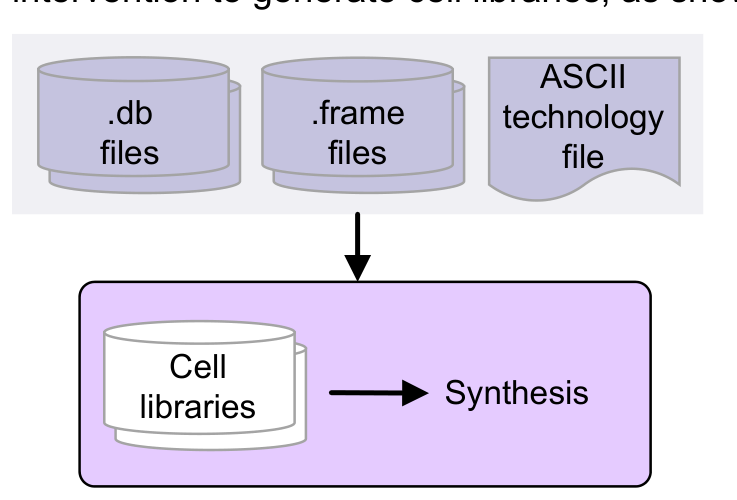
\includegraphics[width=0.70\textwidth,keepaspectratio]{figures/fig-lib-config.png}
\caption{库配置中生成单元库}
\label{fig:lib-config}
\end{figure}

\begin{itemize}
  \item 工具将生成的单元库保存到磁盘，并加入设计库的参考库列表。
  \item 这些单元库与在 Library Manager 中进行库准备时所创建的单元库相同。
\end{itemize}

\begin{seeAlsoBox}
更多信息见 \textit{Fusion Compiler Data Model User Guide} 中的 Configuring Cell Libraries 主题。
\end{seeAlsoBox}

\subsection{限制库单元使用}
\subsubsection*{Restricting Library Cell Usage}

默认情况下，对 block 执行优化或时钟树综合时，Fusion Compiler 可使用单元库中全部可用库单元。要限制单元使用，在 block 已载入内存后使用 \cmd{set\_lib\_cell\_purpose}。该命令具有 block 作用域，并在工具会话间保持；重新打开 block 时会恢复这些设置。

要用 \opt{-include} 与 \opt{-exclude} 选项指定工具可以使用或不可以使用库单元的方式。这两个选项均可接受下列一个或多个取值：\texttt{all}、\texttt{cts}、\texttt{hold}、\texttt{optimization}、\texttt{none}。
\begin{itemize}
  \item \opt{-include} 在指定库单元上设置 \appopt{included\_purposes} 属性。
  \item \opt{-exclude} 在指定库单元上设置 \appopt{excluded\_purposes} 属性。
\end{itemize}

\begin{noteBox}
若库单元带有 \appopt{dont\_use} 属性，则被排除在所有用途之外，效果等同于对该单元执行 \cmd{set\_lib\_cell\_purpose -include none}。
\end{noteBox}

执行优化（含 setup、hold 与逻辑 DRC 修复）时，工具可使用 included purpose 为 \texttt{optimization}、\texttt{hold} 或二者兼有的库单元。执行时钟树综合时，可使用 included purpose 为 \texttt{cts} 的库单元。

例如，禁止某组库单元用于所有用途：
\begin{lstlisting}
fc_shell> set_lib_cell_purpose -include none lib_cells
\end{lstlisting}

仅允许某组库单元用于时钟树综合：
\begin{lstlisting}
fc_shell> set_lib_cell_purpose -include none lib_cells
fc_shell> set_lib_cell_purpose -include cts lib_cells
\end{lstlisting}

允许某组库单元用于除时钟树综合外的所有用途：
\begin{lstlisting}
fc_shell> set_lib_cell_purpose -exclude cts lib_cells
\end{lstlisting}

\subsection{限制所用目标库}
\subsubsection*{Restricting the Target Libraries Used}

默认情况下，优化期间工具可从目标库中选择任意库单元。某些情况下，你可能希望限制用于时钟树综合与优化的库单元。例如，希望在某些设计 block 的优化中排除特定双高度（double-height）单元。

要限制用于时钟树综合与优化的库单元：
\begin{enumerate}
  \item 用 \cmd{set\_target\_library\_subset} 指定库子集。\\
    默认情况下，库子集限制适用于：
    \begin{itemize}
      \item 顶层 block 及其全部子 block。要对特定子 block 设置，使用 \opt{-objects} 选项。
      \item 时钟路径与数据路径二者。要仅对时钟或数据路径设置，分别使用 \opt{-clock} 或 \opt{-data}。
    \end{itemize}
    还可进一步限制目标库子集设置：
    \begin{itemize}
      \item 用 \opt{-dont\_use} 指定库中不应使用的单元列表。
      \item 用 \opt{-only\_here} 指定这些库除指定对象外，不得用于任何其他对象。
    \end{itemize}
  \item 将 \appopt{opt.common.enable\_target\_library\_subset\_opt} 应用选项设为 \texttt{1}，以启用目标库子集。
\end{enumerate}

设置目标库子集时请注意：
\begin{itemize}
  \item 子集限制适用于层次单元，但不适用于叶子单元（leaf cells）。
  \item 命令对指定 block 及其层次中的子设计强制子集限制，但已设置不同子集限制的子设计除外。
  \item 较低层指定的子集会覆盖较高层指定的子集。
\end{itemize}

\begin{figure}[htbp]
\centering
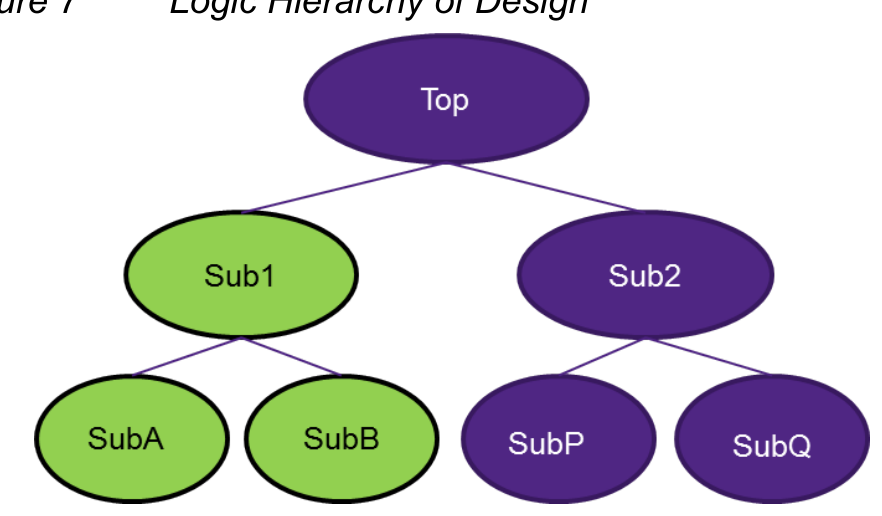
\includegraphics[width=0.92\textwidth,keepaspectratio]{figures/fig-logic-hier.png}
\caption{设计的逻辑层次}
\label{fig:logic-hier}
\end{figure}

例如，假设设计逻辑层次如图~\ref{fig:logic-hier}，希望在优化与时钟树综合中实现如下库限制：
\begin{itemize}
  \item 对 \texttt{Sub1} block 及其子 block \texttt{SubA}、\texttt{SubB}，仅使用名为 \texttt{LVT\_lib} 的库中的单元。
  \item 设计其余部分不得使用该库中的单元。
\end{itemize}

为此使用下列设置：
\begin{lstlisting}
fc_shell> set_target_library_subset -objects {top/Sub1} \
   -only_here [get_lib_cells LVT_lib/*] [get_libs LVT_lib]
fc_shell> set_app_options \
   -name opt.common.enable_target_library_subset_opt -value 1
\end{lstlisting}

除上述设置外，假设还指定：
\begin{lstlisting}
fc_shell> set_lib_cell_purpose -include cts \
   {HVT_lib/buf1 HVT_lib/buf2 LVT_lib/buf1 LVT_lib/buf2}
\end{lstlisting}

则在时钟树综合期间于时钟网络上添加缓冲器时，工具会：
\begin{itemize}
  \item 对名为 \texttt{Sub1} 的 block 及其子 block，使用 \texttt{LVT\_lib} 中的 \texttt{buf1}、\texttt{buf2}；
  \item 对设计其余部分，使用 \texttt{HVT\_lib} 中的 \texttt{buf1}、\texttt{buf2}。
\end{itemize}

\subsubsection{报告目标库子集}
\subsubsection*{Reporting Target Library Subsets}

要查明已为顶层 block 或层次单元定义了哪些目标库子集，使用 \cmd{report\_target\_library\_subset}。

由 \cmd{report\_cells}、\cmd{report\_timing} 等报告命令生成的报告中，对由 \opt{-dont\_use} 或 \opt{-only\_here} 指定的单元会附带 \texttt{td} 属性。

\subsubsection{移除目标库子集}
\subsubsection*{Removing Target Library Subsets}

要从顶层 block 或层次单元移除目标库子集限制，使用 \cmd{remove\_target\_library\_subset}。

% ============================================================
% Fusion Compiler 第 2 章相对 ICC2 新增/显著不同的节（可 \input 片段）
% 原书：Preparing the Design（约 p.80–103、p.135–137）
% ============================================================

\section{指定库子集限制}
\subsection*{Specifying Library Subset Restrictions}

可将时序单元（sequential cells）以及已例化组合单元（instantiated combinational cells）的映射与优化限制到参考库与库单元的某个子集。要指定一个或多个库子集限制，先使用 \cmd{define\_libcell\_subset}，再使用 \cmd{set\_libcell\_subset}。

\begin{noteBox}
库子集限制适用于叶子单元（leaf cells），不适用于层次单元（hierarchical cells）。
\end{noteBox}

要在叶子单元上设置库子集限制：
\begin{enumerate}
  \item 用 \cmd{define\_libcell\_subset} 定义库单元子集。\\
    库单元被分入子集后，不再可用于优化期间的一般映射，而仅用于时序单元与已例化组合单元。
  \item 用 \cmd{set\_libcell\_subset} 限制时序单元与已例化组合单元的优化。\\
    优化期间，工具使用步骤 1 中定义的库子集来优化时序单元（已映射与未映射）以及已映射的组合单元。
\end{enumerate}

下例中，\cmd{define\_libcell\_subset} 将 \texttt{SDFLOP1} 与 \texttt{SDFLOP2} 库单元归入名为 \texttt{special\_flops} 的子集，随后 \cmd{set\_libcell\_subset} 将叶子单元 \texttt{LEAF1} 的映射限制到该 \texttt{special\_flops} 库子集：
\begin{lstlisting}
fc_shell> define_libcell_subset \
   -libcell_list "SDFLOP1 SDFLOP2" -family_name special_flops
fc_shell> set_libcell_subset \
   -object_list "HIER1/LEAF1" -family_name special_flops
\end{lstlisting}

\subsubsection{报告库子集限制}
\subsubsection*{Reporting Library Subset Restrictions}

要报告为时序单元与已例化组合单元指定的库子集，使用 \cmd{report\_libcell\_subset}。

\subsubsection{移除库子集限制}
\subsubsection*{Removing Library Subset Restrictions}

要移除库子集，使用 \cmd{remove\_libcell\_subset}。

% ============================================================


% ============================================================
\section{使用 Pin Access Checker 实用程序}
\subsection*{Using Pin Access Checker Utility}

Pin access checker（PAC）实用程序帮助你在库开发阶段识别 pin 可访问性问题。这有助于改进单元版图——库最终确定并发布给布局布线团队后，将无法再修改单元版图。

布线 DRC 会在布线后识别 pin 访问问题。当单元邻接（abutted）或放置过近时，两个或多个相邻 pin 会争夺公共布线资源，从而引起布线 DRC。

PAC 实用程序的好处包括：
\begin{itemize}
  \item 生成带有多种邻接单元布局排列的布局布线数据库。
  \item 生成布局布线数据库，并根据报告评估所建库的可布局性与 pin 可访问性。
\end{itemize}

PAC 执行下列检查：
\begin{itemize}
  \item 单元布局
  \item 每个库单元 pin 的可访问 track 数量
  \item 布局后的合法化检查
  \item 布线后的设计规则检查
  \item 上述全部检查（含 PG 布线）
\end{itemize}

可用 \cmd{create\_pin\_check\_lib} 根据输入的技术文件与参考库创建或打开新库。PAC 在该库中创建并存储 block。必须通过下列应用选项与 \cmd{create\_pin\_check\_lib} 提供至少三项输入：
\begin{itemize}
  \item 技术文件：用 \opt{-technology} 提供技术文件信息。
  \item 参考库：用 \opt{-ref\_libs} 提供参考库信息。
  \item 金属层布线方向：在 Tcl 脚本中用 \cmd{set\_attribute [get\_layers Mx] routing\_direction horizontal/vertical} 定义布线方向。必须用 \appopt{pin\_check.place.preplace\_option\_file} 应用选项指定该脚本名。
\end{itemize}

要启用 pin access check 实用程序，可使用 \cmd{check\_libcell\_pin\_access}。可用该命令与 \appopt{pin\_check.*} 应用选项启用下列 pin 访问检查：
\begin{itemize}
  \item Legalization
  \item Router
  \item 自动推导单元间距规则（Automatic derivation of cell spacing rule）
\end{itemize}

对 \cmd{check\_libcell\_pin\_access} 使用 \opt{-mode}，通过指定不同 mode 执行多种检查。
\begin{lstlisting}
create_pin_check_lib myTest.nlib -ref_libs ../lib/refLib.ndm \
 -technology ../tf/refTech.tf

set_app_options -as_user_default -name \
 pin_check.place.preplace_option_file -value

check_libcell_pin_access -mode analyze_lib_cell

check_libcell_pin_access -mode analyze_lib_pin

check_libcell_pin_access -mode design_under_test
\end{lstlisting}

若此前使用基于 Tcl 的旧版本，可用 \cmd{translate\_pin\_check\_ui} 将旧脚本转换为新的 Fusion Compiler 命令：
\begin{lstlisting}
translate_pin_check_ui -from old_script.tcl -to new_script.tcl
\end{lstlisting}

\section{分析库}
\subsection*{Analyzing Libraries}

Fusion Compiler 提供下列库分析能力，有助于达成设计的性能、功耗与面积目标：
\begin{itemize}
  \item 识别库单元族（library cell families）中的冗余（redundant）、离群（outlier）与等价（equivalent）单元，可在后续实现流程步骤中将其排除在优化之外。
  \item 识别库单元族中的缺口（gaps），可作为反馈提供给库供应商，以改进参考库。
  \item 比较不同库或同一库不同版本中等价单元的延迟、功耗、面积及其他特性，有助于确定适合设计实现的库。
\end{itemize}

库单元族是共享某些共同属性的单元集合。工具可基于下列方式识别库单元族：
\begin{itemize}
  \item 用户标识的库单元属性，例如功能（function）、阈值电压（threshold voltage）等；
  \item 用户定义的库单元词法属性（lexical attributes）与设置；
  \item 用户指定的自定义库单元族。
\end{itemize}

下图给出执行库分析的高层流程。

\begin{figure}[htbp]
\centering
\fbox{\parbox{0.85\textwidth}{\centering\vspace{1.2cm}
\textit{（原书 Figure 8：Library Analysis Flow）}\\[0.3em]
\small 库分析高层流程；请参阅原版 PDF。
\vspace{1.2cm}}}
\caption{库分析流程}
\label{fig:fc-lib-analysis-flow}
\end{figure}

关于不同类型库分析流程的更多信息，见下列主题：
\begin{itemize}
  \item 库单元族中冗余、离群、等价与缺口简介
  \item 识别库单元族中的冗余、离群、等价与缺口
  \item 比较库
\end{itemize}

\subsection{库单元族中冗余、离群、等价与缺口简介}
\subsubsection*{Introduction to Redundancies, Outliers, Equivalences, and Gaps in Library Cell Families}

当功能相同的单元族按驱动强度（drive strength）递增排序时，特定单元属性值应单调递增或递减。例如，按驱动强度递增排序时，单元面积应单调递增，功耗应递增，而延迟（在相同输出负载与输入 slew 下）应递减。

下图给出功能相同的单元族中，单元面积相对时序的单调分布。

\begin{figure}[htbp]
\centering
\fbox{\parbox{0.85\textwidth}{\centering\vspace{1.2cm}
\textit{（原书 Figure 9：Monotonic Distribution in Library Cell Family）}\\[0.3em]
\small 单元面积相对时序的单调分布；请参阅原版 PDF。
\vspace{1.2cm}}}
\caption{库单元族中的单调分布}
\label{fig:fc-lib-monotonic}
\end{figure}

若某单元的全部度量（如面积、延迟、功耗等）均等于或劣于另一单元，则该单元被视为\textbf{冗余}（redundant），如下图所示（功能相同的单元族中单元面积相对时序的图）。

\begin{figure}[htbp]
\centering
\fbox{\parbox{0.85\textwidth}{\centering\vspace{1.2cm}
\textit{（原书 Figure 10：Redundant Cell in Library Cell Family）}\\[0.3em]
\small 冗余单元示意；请参阅原版 PDF。
\vspace{1.2cm}}}
\caption{库单元族中的冗余单元}
\label{fig:fc-lib-redundant}
\end{figure}

若某单元的度量相对期望值有很大偏差，则该单元被视为\textbf{离群}（outlier），如下图所示（功能相同的单元族中单元面积相对时序的图）。

\begin{figure}[htbp]
\centering
\fbox{\parbox{0.85\textwidth}{\centering\vspace{1.2cm}
\textit{（原书 Figure 11：Outlier Cell in Library Cell Family）}\\[0.3em]
\small 离群单元示意；请参阅原版 PDF。
\vspace{1.2cm}}}
\caption{库单元族中的离群单元}
\label{fig:fc-lib-outlier}
\end{figure}

若单元在所有工艺、电压与温度（process, voltage, and temperature，PVT）取值下全部属性均相同，则这些单元被视为\textbf{等价}（equivalent），如下图所示（功能相同的单元族中单元面积相对时序的图）。

\begin{figure}[htbp]
\centering
\fbox{\parbox{0.85\textwidth}{\centering\vspace{1.2cm}
\textit{（原书 Figure 12：Equivalent Cells in Library Cell Family）}\\[0.3em]
\small 等价单元示意；请参阅原版 PDF。
\vspace{1.2cm}}}
\caption{库单元族中的等价单元}
\label{fig:fc-lib-equivalent}
\end{figure}

当相邻两个驱动强度之间存在很大差异时，即存在\textbf{缺口}（gap），如下图所示（功能相同的单元族中单元面积相对时序的图）。

\begin{figure}[htbp]
\centering
\fbox{\parbox{0.85\textwidth}{\centering\vspace{1.2cm}
\textit{（原书 Figure 13：Gap in Library Cell Family）}\\[0.3em]
\small 驱动强度缺口示意；请参阅原版 PDF。
\vspace{1.2cm}}}
\caption{库单元族中的缺口}
\label{fig:fc-lib-gap}
\end{figure}

\subsection{识别库单元族中的冗余、离群、等价与缺口}
\subsubsection*{Identifying Redundancies, Outliers, Equivalences, and Gaps in Library Cell Families}

要识别单元族中的冗余、离群、等价与缺口，执行下列步骤：

\begin{enumerate}
  \item 用 \cmd{create\_libset} 创建待分析库的集合（称为 \textbf{libset}），例如：
\begin{lstlisting}
fc_shell> create_libset -name myLibset -libs {abcd1 abcd2}
\end{lstlisting}
    执行库分析时，可指定 libset 名，而不必指定库列表。此外，工具在分析期间生成报告、绘图等时也使用 libset 名，而非库名列表。\\
    可将同一单元库包含在多个 libset 中。

  \item 用 \cmd{create\_environment} 设置库分析环境。\\
    \cmd{create\_environment} 将预定义的 libset 与工艺标签（process label）、工艺编号（process number）、电压与温度关联，随后用于分析库。\\
    可用下列方法之一指定分析环境的工艺标签、工艺编号、电压与温度：
    \begin{itemize}
      \item 用 \opt{-ppvt} 直接指定工艺标签、工艺编号、电压与温度，例如：
\begin{lstlisting}
fc_shell> create_environment -name env1 -libset myLibset \
   -ppvt {{SS1p, 1.0, 0.6, 125}}
\end{lstlisting}
      \item 用 \opt{-op\_conds} 指定参考库中的预定义工作条件，例如：
\begin{lstlisting}
fc_shell> create_environment -name env2 -libset myLibset \
   -op_conds SS1p6125
\end{lstlisting}
      \item 用 \opt{-corners} 指定 corner，由工具从中推断工艺标签、工艺编号、电压与温度，例如：
\begin{lstlisting}
fc_shell> create_environment -name env3 -libset myLibset \
   -corners nworst
\end{lstlisting}
      \item 用 \opt{-auto\_infer\_design} 指定由工具从当前设计关联的 scenario 与 UPF 推断工艺标签、工艺编号、电压与温度，例如：
\begin{lstlisting}
fc_shell> create_environment -name env4 -libset myLibset \
   -auto_infer_design
\end{lstlisting}
    \end{itemize}

  \item （可选）为库单元指定命名约定，并用词法属性执行词法分类（lexical classification）。\\
    库单元命名约定有助于工具在后续流程步骤中识别单元族。\\
    例如，假定库中某单元名为 \texttt{AND2D4WSULVT}。该名称是 \texttt{AND2}、\texttt{D4}、\texttt{WS} 与 \texttt{ULVT} 字符串的拼接，分别表示与某词法属性关联的单元特性，如下表所示：

\begin{table}[htbp]
\centering
\caption{示例库命名约定的词法属性}
\label{tab:fc-lexical-attrs-1}
\begin{tabularx}{\textwidth}{@{}c l X l@{}}
\toprule
\textbf{列} & \textbf{词法属性} & \textbf{允许模式} & \textbf{示例单元取值} \\
\midrule
1 & \texttt{lexical\_cell\_prefix\_name} & \texttt{[a-zA-Z0-9]*} & \texttt{AND2} \\
2 & \texttt{lexical\_drive1\_name} & \texttt{D[0-9]*} & \texttt{D4} \\
3 & \texttt{lexical\_well\_substrate\_bias\_architecure} & \texttt{WS} & \texttt{WS} \\
4 & \texttt{lexical\_device\_threshold\_voltage} & \texttt{ULVT | SVT | LVT | MVT} & \texttt{ULVT} \\
\bottomrule
\end{tabularx}
\end{table}

    可用 \cmd{set\_lib\_cell\_naming\_convention} 为该库指定命名约定，例如：
\begin{lstlisting}
fc_shell> set_lib_cell_naming_convention -library $lib \
   -column 1 -pattern {[a-zA-Z0-9]*} -attribute \
   "lexical_cell_prefix_name"
fc_shell> set_lib_cell_naming_convention -library $lib \
   -column 2 -pattern {D[0-9]*} -attribute "lexical_drive1_name"
fc_shell> set_lib_cell_naming_convention -library $lib \
   -column 3 -pattern {WS} -attribute \
   "lexical_well_substrate_bias_architecure"
fc_shell> set_lib_cell_naming_convention -library $lib \
   -column 4 -pattern {ULVT|SVT|LVT|MVT} -attribute \
   "lexical_device_threshold_voltage"
\end{lstlisting}

\begin{noteBox}
预定义词法属性的完整列表见 \cmd{set\_lib\_cell\_naming\_convention} 命令的 man page。
\end{noteBox}

    指定命名约定后，用 \cmd{classify\_lib\_cell\_attributes} 执行词法分类，例如：
\begin{lstlisting}
fc_shell> classify_lib_cell_attributes -libset myLibset
\end{lstlisting}
    要用 \cmd{report\_lib\_cell\_classification\_attributes} 报告词法分类结果。\\
    要用 \cmd{report\_lexical\_unclassified\_lib\_cells} 报告在给定命名约定下未被词法分类的库单元。若存在未分类单元，请补充命名约定并重新运行词法分类。

  \item （可选）用 \cmd{set\_use\_for\_library\_analysis} 将特定单元排除在库分析之外。\\
    默认情况下，工具在库分析期间排除仅物理单元（physical-only cells）。但你可排除更多单元，例如带有 \texttt{dont\_use} 设置的库单元：
\begin{lstlisting}
fc_shell> set exclude_cells [filter_collection [get_lib_cells $libs/*] \
   "dont_use == true"]
fc_shell> set_use_for_library_analysis $exclude_cells false
\end{lstlisting}
    要用 \cmd{report\_lexical\_ignored\_lib\_cells} 报告被排除的单元。

  \item 用 \cmd{identify\_lib\_cell\_families} 识别全部库单元族。\\
    要用 \cmd{report\_lib\_cell\_families -all\_initial} 报告工具识别的库单元族。\\
    要手动定义库单元族，使用 \cmd{define\_lib\_cell\_family}。要用 \cmd{report\_lib\_cell\_families -all\_userdef} 报告这些用户定义的单元族。

  \item 用 \cmd{run\_library\_analysis} 分析库，例如：
\begin{lstlisting}
fc_shell> run_library_analysis -name myLibset_run1 -environment env1
\end{lstlisting}
    用 \opt{-environment} 指定的环境名必须对应先前用 \cmd{create\_environment} 创建的环境。

  \item 用 \cmd{find\_library\_redundancies} 识别库单元族中的冗余，例如：
\begin{lstlisting}
fc_shell> find_library_redundancies -analysis myLibset_run1
\end{lstlisting}
    用 \opt{-analysis} 指定的分析名必须对应先前用 \cmd{run\_library\_analysis} 执行的分析。\\
    除冗余单元外，\cmd{find\_library\_redundancies} 还会识别库单元族中的离群单元与等价单元。

  \item 用 \cmd{find\_library\_gaps} 识别库单元族中的缺口，例如：
\begin{lstlisting}
fc_shell> find_library_gaps -analysis myLibset_run1
\end{lstlisting}
    用 \opt{-analysis} 指定的分析名必须对应先前用 \cmd{run\_library\_analysis} 执行的分析。

  \item 用 \cmd{report\_library\_analysis} 报告库分析期间识别的库单元缺口、冗余、离群与等价，例如：
\begin{lstlisting}
fc_shell> report_library_analysis -analysis myLibset_run1 \
   -analysis_type redundancy -detail
fc_shell> report_library_analysis -analysis myLibset_run1 \
   -analysis_type outlier -detail
fc_shell> report_library_analysis -analysis myLibset_run1 \
   -analysis_type equivalent -detail
fc_shell> report_library_analysis -analysis myLibset_run1 \
   -analysis_type gap -detail
\end{lstlisting}

  \item 用 \cmd{gui\_plot\_lib\_cells\_attributes} 生成绘图，例如：
\begin{lstlisting}
fc_shell> gui_plot_lib_cells_attributes -libset myLibset \
  -lib_cell_type all -x_attrib_name leakage -y_attrib_name \
  avgsl_fall_delay \
  -chart_type scatter
\end{lstlisting}
\end{enumerate}

\subsection{比较库}
\subsubsection*{Comparing Libraries}

要比较库，执行下列步骤：

\begin{enumerate}
  \item 用 \cmd{create\_libset} 创建待分析库的集合（libset），例如：
\begin{lstlisting}
fc_shell> create_libset -name myLibset -libs {abcd1.db abcd2.db}
\end{lstlisting}
    执行库分析时，可指定 libset 名，而不必指定库列表。此外，工具在分析期间生成报告、绘图等时也使用 libset 名，而非库名列表。\\
    可将同一单元库包含在多个 libset 中。

  \item 用 \cmd{create\_environment} 设置库分析环境。\\
    \cmd{create\_environment} 将预定义的 libset 与工艺标签、工艺编号、电压与温度关联，随后用于分析库。\\
    可用下列方法之一指定分析环境的工艺标签、工艺编号、电压与温度：
    \begin{itemize}
      \item 用 \opt{-ppvt} 直接指定工艺标签、工艺编号、电压与温度，例如：
\begin{lstlisting}
fc_shell> create_environment -name env1 -libset myLibset \
   -ppvt {{SS1p, 1.0, 0.6, 125}}
\end{lstlisting}
      \item 用 \opt{-op\_conds} 指定参考库中的预定义工作条件，例如：
\begin{lstlisting}
fc_shell> create_environment -name env2 -libset myLibset \
   -op_conds SS1p6125
\end{lstlisting}
      \item 用 \opt{-corners} 指定 corner，由工具从中推断工艺标签、工艺编号、电压与温度，例如：
\begin{lstlisting}
fc_shell> create_environment -name env3 -libset myLibset \
   -corners nworst
\end{lstlisting}
      \item 用 \opt{-auto\_infer\_design} 指定由工具从当前设计关联的 scenario 与 UPF 推断工艺标签、工艺编号、电压与温度，例如：
\begin{lstlisting}
fc_shell> create_environment -name env4 -libset myLibset \
   -auto_infer_design
\end{lstlisting}
    \end{itemize}

  \item （可选）为库单元指定命名约定，并用词法属性执行词法分类。\\
    库单元命名约定有助于工具在后续流程步骤中识别单元族。\\
    例如，假定库中某单元名为 \texttt{AND2D4WSULVT}。该名称是 \texttt{AND2}、\texttt{D4}、\texttt{WS} 与 \texttt{ULVT} 字符串的拼接，分别表示与某词法属性关联的单元特性，如下表所示：

\begin{table}[htbp]
\centering
\caption{示例库命名约定的词法属性（比较库）}
\label{tab:fc-lexical-attrs-2}
\begin{tabularx}{\textwidth}{@{}c l X l@{}}
\toprule
\textbf{列} & \textbf{词法属性} & \textbf{允许模式} & \textbf{示例单元取值} \\
\midrule
1 & \texttt{lexical\_cell\_prefix\_name} & \texttt{[a-zA-Z0-9]*} & \texttt{AND2} \\
2 & \texttt{lexical\_drive1\_name} & \texttt{D[0-9]*} & \texttt{D4} \\
3 & \texttt{lexical\_well\_substrate\_bias\_architecure} & \texttt{WS} & \texttt{WS} \\
4 & \texttt{lexical\_device\_threshold\_voltage} & \texttt{ULVT | SVT | LVT | MVT} & \texttt{ULVT} \\
\bottomrule
\end{tabularx}
\end{table}

    可用 \cmd{set\_lib\_cell\_naming\_convention} 为该库指定命名约定，例如：
\begin{lstlisting}
fc_shell> set_lib_cell_naming_convention -library $lib \
   -column 1 -pattern {[a-zA-Z0-9]*} -attribute \
   "lexical_cell_prefix_name"
fc_shell> set_lib_cell_naming_convention -library $lib \
   -column 2 -pattern {D[0-9]*} -attribute "lexical_drive1_name"
fc_shell> set_lib_cell_naming_convention -library $lib \
   -column 3 -pattern {WS} -attribute \
   "lexical_well_substrate_bias_architecure"
fc_shell> set_lib_cell_naming_convention -library $lib \
   -column 4 -pattern {ULVT|SVT|LVT|MVT} -attribute \
   "lexical_device_threshold_voltage"
\end{lstlisting}

\begin{noteBox}
预定义词法属性的完整列表见 \cmd{set\_lib\_cell\_naming\_convention} 命令的 man page。
\end{noteBox}

    指定命名约定后，用 \cmd{classify\_lib\_cell\_attributes} 执行词法分类，例如：
\begin{lstlisting}
fc_shell> classify_lib_cell_attributes -libset myLibset
\end{lstlisting}
    要用 \cmd{report\_lib\_cell\_classification\_attributes} 报告词法分类结果。\\
    要用 \cmd{report\_lexical\_unclassified\_lib\_cells} 报告在给定命名约定下未被词法分类的库单元。若存在未分类单元，请补充命名约定并重新运行词法分类。

  \item （可选）用 \cmd{set\_use\_for\_library\_analysis} 将特定单元排除在库分析之外。\\
    默认情况下，工具在库分析期间排除仅物理单元。但你可排除更多单元，例如带有 \texttt{dont\_use} 设置的库单元：
\begin{lstlisting}
fc_shell> set exclude_cells [filter_collection [get_lib_cells $libs/*] \
   "dont_use == true"]
fc_shell> set_use_for_library_analysis $exclude_cells false
\end{lstlisting}
    要用 \cmd{report\_lexical\_ignored\_lib\_cells} 报告被排除的单元。

  \item 用 \cmd{identify\_lib\_cell\_families} 识别全部库单元族。\\
    要用 \cmd{report\_lib\_cell\_families -all\_initial} 报告工具识别的库单元族。\\
    要手动定义库单元族，使用 \cmd{define\_lib\_cell\_family}；要用 \cmd{report\_lib\_cell\_families -all\_userdef} 报告这些用户定义的单元族。

  \item 用 \cmd{run\_library\_analysis} 分析库，例如：
\begin{lstlisting}
fc_shell> run_library_analysis -name myLibset_run1 -environment env1
\end{lstlisting}
    用 \opt{-environment} 指定的环境名必须对应先前用 \cmd{create\_environment} 创建的环境。

  \item 用 \cmd{compare\_libraries} 比较库。\\
    此时必须用 \opt{-ref\_lib} 与 \opt{-target\_lib} 指定要比较的两个库。此外，必须用 \opt{-ref\_lib\_analysis} 与 \opt{-target\_lib\_analysis} 为每个库指定先前用 \cmd{run\_library\_analysis} 执行的库分析运行名，例如：
\begin{lstlisting}
fc_shell> compare_libraries -ref_lib $rvt_lib -ref_lib_analysis sa \
   -target_lib $lvt_lib -target_lib_analysis sa -verbose -plot
\end{lstlisting}
    比较库时，可能遇到下列与参考库、目标库单元名称匹配相关的情况：
    \begin{itemize}
      \item 参考库与目标库中的单元名可完全匹配，例如同一库的两个不同版本。此时无需额外词法分类。
      \item 参考库与目标库可具有相同命名约定，但其中一个库的词法属性较少。\\
        例如，假定参考库中名为 \texttt{ND2D1SVT} 的单元与目标库中名为 \texttt{ND2D1} 的单元匹配。此时目标库单元名不含 \texttt{lexical\_device\_threshold\_voltage} 属性，如下表所示。

\begin{table}[htbp]
\centering
\caption{参考库与目标库词法属性差异（属性缺失）}
\label{tab:fc-lex-diff-missing}
\begin{tabularx}{\textwidth}{@{}X l l@{}}
\toprule
\textbf{词法属性} & \textbf{参考库} & \textbf{目标库} \\
\midrule
\texttt{lexical\_cell\_prefix\_name} & \texttt{ND2} & \texttt{ND2} \\
\texttt{lexical\_drive1\_name} & \texttt{D1} & \texttt{D1} \\
\texttt{lexical\_device\_threshold\_voltage} & \texttt{SVT} & --- \\
\bottomrule
\end{tabularx}
\end{table}

        在此情况下，比较两个库时应忽略 \texttt{lexical\_device\_threshold\_voltage} 属性。为此，在运行 \cmd{compare\_libraries} 之前使用下列应用选项设置：
\begin{lstlisting}
fc_shell> set_app_options -name libra.complib.match_full_cell_name \
 -value false
fc_shell> set_app_options -name \
 libra.complib.match_lexical_device_threshold_voltage -value false
fc_shell> compare_libraries -ref_lib $rvt_lib -ref_lib_analysis sa \
   -target_lib $lvt_lib -target_lib_analysis sa -verbose -plot
\end{lstlisting}

\begin{noteBox}
控制库比较期间名称匹配的应用选项完整列表见 \cmd{compare\_libraries} 命令的 man page。
\end{noteBox}

      \item 参考库与目标库可具有相似命名约定，但词法属性取值可能并不相同。\\
        例如，假定参考库中名为 \texttt{ND2D1SVT} 的单元与目标库中名为 \texttt{nand2\_svth\_x1} 的单元匹配。此时两库具有相同词法属性，但取值相似而不完全相同，如下表所示。

\begin{table}[htbp]
\centering
\caption{参考库与目标库词法属性差异（取值不同）}
\label{tab:fc-lex-diff-values}
\begin{tabularx}{\textwidth}{@{}X l l@{}}
\toprule
\textbf{词法属性} & \textbf{参考库} & \textbf{目标库} \\
\midrule
\texttt{lexical\_cell\_prefix\_name} & \texttt{ND2} & \texttt{nand2} \\
\texttt{lexical\_drive1\_name} & \texttt{D1} & \texttt{x1} \\
\texttt{lexical\_device\_threshold\_voltage} & \texttt{SVT} & \texttt{svth} \\
\bottomrule
\end{tabularx}
\end{table}

        在此情况下，必须创建包含下列信息的词法属性映射文件：
\begin{lstlisting}
lexical_cell_prefix_name      ND2  nand2
lexical_drive1_name               D1   x1
lexical_device_threshold_voltage  SVT  svth
\end{lstlisting}
        然后，运行 \cmd{compare\_libraries} 时必须用 \opt{-lex\_attr\_mapping} 指定该词法属性映射文件，例如：
\begin{lstlisting}
fc_shell> set_app_options -name libra.complib.match_full_cell_name \
 -value false
fc_shell> compare_libraries -ref_lib $rvt_lib -ref_lib_analysis sa \
   -target_lib $lvt_lib -target_lib_analysis sa \
   -lex_attr_mapping attribute_map_file -verbose -plot
\end{lstlisting}

      \item 参考库与目标库的命名约定完全不同。\\
        在此情况下，必须创建包含待比较单元对的自定义映射文件，例如：
\begin{lstlisting}
INVD2BWP     INVD1BWPHVT
INVD2BWP     BUFFD4BWPHVT
ND2D2BWP     ND2D4BWPHVT
DFQD4BWP     SDFQD4BWPHVT
\end{lstlisting}
        然后，运行 \cmd{compare\_libraries} 时必须用 \opt{-custom\_pairs} 指定该映射文件，例如：
\begin{lstlisting}
fc_shell> set_app_options -name libra.complib.match_full_cell_name \
 -value false
fc_shell> compare_libraries -ref_lib $rvt_lib -ref_lib_analysis sa \
   -target_lib $lvt_lib -target_lib_analysis sa \
   -custom_pairs custom_map_file -verbose -plot
\end{lstlisting}
    \end{itemize}
\end{enumerate}

% ============================================================
\section{读取设计}
\subsection*{Reading the Design}

读取设计之前，必须创建或打开与该设计关联的设计库，见「设置库」（Setting Up Libraries）。

工具可读取 SystemVerilog、Verilog 或 VHDL 格式的 RTL 设计，以及 Verilog 格式的门级网表（gate-level netlists）。

用下列方法读取设计：
\begin{itemize}
  \item 以 SystemVerilog、Verilog 或 VHDL 格式读取 RTL 文件
  \item 使用 \opt{-autoread} 选项读取设计
  \item 使用 VCS 命令行选项读取设计
  \item 读取 Verilog 门级网表文件
  \item 读取混合的门级网表与 RTL 文件
\end{itemize}

默认情况下，工具读取 RTL 或门级网表文件时，会在当前设计库中创建一个 block，并增加其打开计数。工具通过识别在指定文件中未被其他模块例化的模块来确定 block 的顶层模块，并以该顶层模块名作为 block 名。

用下列命令处理 block：
\begin{itemize}
  \item \cmd{create\_block}：创建 block
  \item \cmd{open\_block}：打开已有 block
  \item \cmd{current\_block}：设置或报告当前 block
  \item \cmd{save\_block}：保存 block
  \item \cmd{close\_blocks}：关闭 block
\end{itemize}

\begin{seeAlsoBox}
参见：Blocks；Working With Design Libraries。
\end{seeAlsoBox}

\subsection{以 SystemVerilog、Verilog 或 VHDL 格式读取 RTL 文件}
\subsubsection*{Reading RTL Files in SystemVerilog, Verilog, or VHDL Format}

使用 \cmd{analyze} 与 \cmd{elaborate} 命令，随后使用 \cmd{set\_top\_module}。

\cmd{analyze} 会根据 \opt{-hdl\_library} 选项提供的库名，在磁盘上自动创建 HDL 模板库（HDL template libraries）。HDL 模板库的位置由 \appopt{hdlin.hdl\_library.default\_dirname} 应用选项控制。未指定 \opt{-hdl\_library} 时，默认库名为 \texttt{WORK}。要用 \appopt{hdlin.hdl\_library.default\_name} 指定不同的默认库名。

\begin{noteBox}
控制 RTL 读取行为的全部应用选项均带有 \texttt{hdlin} 前缀。
\end{noteBox}

\cmd{elaborate} 构建指定模块，但不链接设计的其余部分。设计链接只能在整个设计都已在内存中之后执行，因此 \cmd{elaborate} 不执行链接。这允许在对整个设计执行一次链接之前运行多次 \cmd{elaborate}。顶层模块必须是已 elaborate 的模块之一。

用 \cmd{set\_top\_module} 完成设计链接并设置顶层模块。顶层模块作为参数传给 \cmd{set\_top\_module}。顶层模块必须是先前用 \cmd{elaborate} 已 elaborate 的模块。\cmd{set\_top\_module} 将指定模块设为顶层设计，链接整个设计，并创建一个供后续综合流程使用的单一 block。

下列脚本用模板库读取 VHDL 文件并创建名为 \texttt{top} 的 block。无需指定磁盘上模板库的位置；\cmd{analyze} 会根据 \opt{-hdl\_library} 自动创建：
\begin{lstlisting}
analyze -format vhdl -hdl_library BOT_HDL_LIB bot.vhd
analyze -format vhdl -hdl_library MID_HDL_LIB mid.vhd
analyze -format vhdl top.vhd
elaborate top
set_top_module top
\end{lstlisting}

若顶层设计被分析到默认库以外的 HDL 模板库，应用 \opt{-hdl\_library} 为顶层设计提供 HDL 模板库名。例如：
\begin{lstlisting}
analyze -format vhdl -hdl_library BOT_HDL_LIB bot.vhd
analyze -format vhdl -hdl_library MID_HDL_LIB mid.vhd
analyze -format vhdl -hdl_library TOP_HDL_LIB top.vhd
elaborate -hdl_library TOP_HDL_LIB top
set_top_module top
\end{lstlisting}

也可选用 \cmd{define\_hdl\_library} 指定磁盘上 HDL 模板库的位置。例如：
\begin{lstlisting}
define_hdl_library BOT_HDL_LIB -path ./TEMPLATES/BOT_HDL_LIB
define_hdl_library MID_HDL_LIB -path ./TEMPLATES/MID_HDL_LIB
define_hdl_library WORK -path ./TEMPLATES/WORK
analyze -format vhdl -hdl_library BOT_HDL_LIB bot.vhd
analyze -format vhdl -hdl_library MID_HDL_LIB mid.vhd
analyze -format vhdl top.vhd
elaborate top
set_top_module top
\end{lstlisting}

\subsection{使用 \texttt{-autoread} 选项读取设计}
\subsubsection*{Reading Designs Using the -autoread Option}

要让工具自动读取 RTL 文件列表，对 \cmd{analyze} 指定 \opt{-autoread}，如下例所示。指定该选项时，用于分析 RTL 文件的 RTL 语言由文件扩展名自动确定。要用下列应用选项控制文件扩展名：\appopt{hdlin.autoread.verilog\_extensions}、\appopt{hdlin.autoread.sverilog\_extensions}、\appopt{hdlin.autoread.vhdl\_extensions} 以及 \appopt{hdlin.autoread.exclude\_extensions}。
\begin{lstlisting}
set DESIGN_NAME top
analyze -autoread -top ${DESIGN_NAME} ${RTL_FILE_LIST}
elaborate ${DESIGN_NAME}
elaborate -hdl_library TOP_HDL_LIB top
set_top_module ${DESIGN_NAME}
\end{lstlisting}

\subsection{使用 VCS 命令行选项读取设计}
\subsubsection*{Reading Designs Using the VCS Command-line Options}

带 VCS 命令行选项的 \cmd{analyze} 提供与 VCS 仿真脚本的兼容性，并便于读取大型设计。使用 VCS 命令行选项时，工具通过在指定库中搜索被引用设计并加载这些设计，自动解析已例化设计的引用（references）。

要读取包含大量 HDL 源文件与库的设计，对 \cmd{analyze} 指定 \opt{-vcs}。必须将 VCS 命令行选项括在双引号中。

例如：
\begin{lstlisting}
analyze -vcs "-verilog -y mylibdir1 +libext+.v -v myfile1 \
   +incdir+myincludedir1 -f mycmdfile2" top.v
elaborate ${DESIGN_NAME}
set_top_module ${DESIGN_NAME}
\end{lstlisting}

要在同一次 \cmd{analyze} 中读取指定扩展名的 SystemVerilog 文件与 Verilog 文件，使用 \opt{-vcs "+systemverilogext+ext"}。此时文件不得包含任何 Verilog 2001 风格。

例如，下列命令分析扩展名为 \texttt{.sv} 的 SystemVerilog 文件以及 Verilog 文件：
\begin{lstlisting}
analyze -format verilog -vcs "-f F +systemverilogext+.sv"
elaborate ${DESIGN_NAME}
set_top_module ${DESIGN_NAME}
\end{lstlisting}

\subsection{读取 Verilog 门级网表文件}
\subsubsection*{Reading Verilog Gate-Level Netlist Files}

用 \cmd{read\_verilog} 通过专用 Verilog 网表读取器读取 Verilog 网表文件。该命令不能用于读取 Verilog RTL 文件。读取 RTL 文件应仅使用 \cmd{analyze} 与 \cmd{elaborate}。读取网表后使用 \cmd{set\_top\_module} 指定顶层模块并链接设计以创建 block。
\begin{lstlisting}
read_verilog top.netlist.v
set_top_module top
\end{lstlisting}

当文件含有多个独立模块时，用 \opt{-top} 标识顶层模块。例如：
\begin{lstlisting}
read_verilog -top top2 netlists.v
set_top_module top2
\end{lstlisting}

要指定不同于 \texttt{top\_module\_name.design} 的新 block 名，使用 \opt{-design}。例如：
\begin{lstlisting}
read_verilog -top my_top -design desA ../my_data/my_des.v
set_top_module my_top
\end{lstlisting}

\subsection{读取混合的门级网表与 RTL 文件}
\subsubsection*{Reading Mixed Gate-Level Netlists and RTL Files}

可以读取 Verilog 网表与 RTL 文件的组合。用 \cmd{read\_verilog} 读取 Verilog 网表；用 \cmd{analyze} 与 \cmd{elaborate} 读取 RTL 文件。全部网表文件与 RTL 文件读入工具后，用 \cmd{set\_top\_module} 链接设计以创建用于综合的 block。

下例说明如何读取网表与 RTL 的混合。如本例所示，带参数 elaborate 顶层模块时，顶层模块名也会包含参数化模块名。可用下列应用选项控制参数化模块的命名风格：\appopt{hdlin.naming.template\_naming\_style}、\appopt{hdlin.naming.template\_parameter\_style} 以及 \appopt{hdlin.naming.template\_separator\_style}。
\begin{lstlisting}
# Read netlist files
read_verilog NETLIST/bot.v
# Analyze design files
analyze -format sverilog -hdl_library MID RTL/mid.sv
analyze -format sverilog                  RTL/top.svd
# Elaborate top design module
elaborate -parameters "N=8,M=3" top
# Set the top level module to resolve references
set_top_module top_N8_M3
\end{lstlisting}

\subsection{在 RTL 代码中嵌入 Tcl 命令}
\subsubsection*{Embedding Tcl Commands in RTL Code}

要在 RTL 代码中嵌入 Tcl 命令，使用 \texttt{fc\_tcl\_script\_begin} 与 \texttt{fc\_tcl\_script\_end} 指令。下列 Tcl 命令可嵌入 RTL 设计：
\begin{itemize}
  \item \cmd{set\_attribute}
  \item \cmd{set\_ungroup}
  \item \cmd{set\_size\_only}
  \item \cmd{set\_dont\_touch}
  \item \cmd{set\_dont\_retime}
  \item \cmd{set\_implementation}
  \item \cmd{set\_optimize\_registers}
  \item \cmd{get\_modules}
  \item \cmd{get\_cells}
  \item \cmd{get\_pins}
  \item \cmd{get\_nets}
  \item \cmd{get\_ports}
\end{itemize}

下列 RTL 示例包含嵌入的 Tcl 命令，对名称前缀为 \texttt{iPort1.dout\_reg} 的全部寄存器施加 \texttt{size\_only} 设置：
\begin{lstlisting}
module bot ( myIntf1.datIn iPort1 );
  always @(posedge iPort1.clk or negedge iPort1.rst)
  begin
    if (iPort1.rst == 1'b0)
    begin
      iPort1.dout <= '0;
    end else begin
      iPort1.dout <= iPort1.iData1 + iPort1.iData2;
    end
  end
// synopsys fc_tcl_script_begin
// set_size_only [get_cells iPort1.dout_reg*]
// synopsys fc_tcl_script_end
endmodule
\end{lstlisting}

% ============================================================
\section{缓解设计不匹配}
\subsection*{Mitigating Design Mismatches}

在早期设计开发中，频繁的设计更新可能导致数据不完整或不一致，例如 block 级设计与顶层设计对其引用之间的 pin 不匹配。要让工具即使存在某些类型的设计不匹配（design mismatch）仍能成功链接 block，可为该 block 设置不匹配配置（mismatch configuration）。

默认情况下，工具无法链接带有不一致或不匹配数据的任何 block。设置不匹配配置后，工具会忽略或修复若干不同类型的不匹配数据，并继续链接过程。以不匹配数据链接的 block 仅可用于可行性分析（feasibility analysis）。

\begin{seeAlsoBox}
关于如何缓解设计不匹配，见 \textit{Fusion Compiler Data Model User Guide}。
\end{seeAlsoBox}

% ============================================================


% ============================================================
\section{处理设计（门级网表与 block 操作补充）}
\subsection*{Working With Designs}

\begin{noteBox}
Fusion Compiler 推荐优先使用上一节「读取设计」中的 \cmd{read\_rtl}/\cmd{analyze}/\cmd{elaborate} 等流程。下列内容保留门级网表读取与 block 操作要点，与原 ICC2 流程兼容。
\end{noteBox}

在多数情况下，在 Fusion Compiler 中处理设计时，使用设计库中某一版本（block）的 design view。本手册中，\textbf{block} 指设计库中的特定设计版本（不论顶层设计还是子设计）；\textbf{design} 泛指正在处理的设计。除非另有说明，二者均指 design view。

Fusion Compiler 以 Verilog 格式读取设计。Verilog 网表文件是单个文件中的结构级或门级设计。要将设计读入 Fusion Compiler：
\begin{enumerate}
  \item 创建或打开与该设计关联的设计库。
    \begin{itemize}
      \item 若设计库尚不存在，用 \cmd{create\_lib} 创建。
      \item 若设计库已存在，用 \cmd{open\_lib} 打开。
    \end{itemize}
  \item 用 \cmd{read\_verilog} 读取设计的 Verilog 网表文件。\\
    默认情况下，工具读取 Verilog 网表时会在当前设计库中创建一个 block，并增加其打开计数。工具通过识别在指定 Verilog 文件中未被其他模块例化的模块来确定 block 的顶层模块，并以该顶层模块名作为 block 名。\\
    工具还会为 block 创建默认电源域（power domain）。对多电压设计，在指定功耗意图（power intent）时该默认电源域会被替换，见「加载并应用 UPF 信息」。
\end{enumerate}

用下列命令处理 block：
\begin{itemize}
  \item \cmd{create\_block}：创建 block
  \item \cmd{open\_block}：打开已有 block
  \item \cmd{current\_block}：设置或报告当前 block
  \item \cmd{save\_block}：保存 block
  \item \cmd{close\_blocks}：关闭 block
\end{itemize}

\begin{seeAlsoBox}
参见：Blocks；Working With Design Libraries。
\end{seeAlsoBox}

% ============================================================
\section{导入 Floorplan 信息}
\subsection*{Importing the Floorplan Information}

Floorplan 包含物理约束，例如 core 区域与形状、port 位置、宏单元位置与方向等，这些是执行物理综合与优化所必需的。

若 block 已有 floorplan，按「读取 DEF 文件」所述将其作为 DEF 文件读入。

若 block 尚无 floorplan，可按 \textit{Fusion Compiler Design Planning User Guide} 所述执行设计规划并生成 floorplan。

\subsection{读取 DEF 文件}
\subsubsection*{Reading DEF Files}

要从 DEF 文件读取 floorplan 信息，使用 \cmd{read\_def}：
\begin{lstlisting}
fc_shell> read_def block.def
\end{lstlisting}

\begin{noteBox}
尽可能使用 DEF v5.8 或更高版本，因为该版本比早期版本支持更多类型的物理对象与障碍物（obstructions）。
\end{noteBox}

默认情况下，\cmd{read\_def} 命令会：
\begin{itemize}
  \item 将 floorplan 信息标注到当前 block。\\
    要标注到其他 block，用 \opt{-design} 指定 block 名。
  \item 保留已有 floorplan 信息。\\
    在增量（incremental）模式下：
    \begin{itemize}
      \item 布局区域根据当前 core 区域以及 DEF 中的 site rows 导入；
      \item 只能有一个取值的物理约束会被最新 DEF 中的值覆盖，例如 port 位置与宏单元位置会被覆盖；
      \item 可累积取值的物理约束会重新计算，即 core 区域可根据已有值与最新 DEF 中的 site row 定义重新计算。不同 DEF 文件中的 placement keepout 会累积，最终 keepout 几何在综合期间由内部计算。
    \end{itemize}
    要在标注 DEF 中的 floorplan 信息之前先清除已有 floorplan，使用 \opt{-no\_incremental}。该模式下，布局区域根据 DEF 中的 site rows 导入。
  \item 对宏单元与 port 使用基于规则的名称匹配（rule-based name matching）。\\
    基于规则的名称匹配利用工具的智能名称匹配能力自动解决名称差异。启用时，默认下列字符视为等价：
    \begin{itemize}
      \item 层次分隔符 \texttt{\{ / \_ . \}}\\
        例如，名为 \texttt{a.b\_c/d\_e} 的单元会自动与 DEF 中的字符串 \texttt{a/b\_c.d/e} 匹配。
      \item 总线记号 \texttt{\{ [ ] \_\_ ( ) \}}\\
        例如，名为 \texttt{a [4] [5]} 的单元会自动与 DEF 中的 \texttt{a\_4\_\_5\_} 匹配。
    \end{itemize}
    要禁用基于规则的名称匹配并要求 DEF 与 block 之间精确名称匹配，将 \appopt{file.def.rule\_based\_name\_matching} 设为 \texttt{false}。

\begin{seeAlsoBox}
更多信息见 \textit{Fusion Compiler Data Model User Guide} 中的 ``Rule-Based Name Matching''。
\end{seeAlsoBox}

  \item 忽略 DEF 中存在但 block 中不存在的任何对象（PG 对象除外）。\\
    要允许从 DEF 创建新的非 PG 对象，用 \opt{-add\_def\_only\_objects} 指定要创建的对象类型。指定下列一个或多个关键字：
    \begin{itemize}
      \item \texttt{cells}：工具创建仅存在于 DEF 中的单元，并按 DEF 定义连接其电源与地 pin；即使 DEF 中定义了信号、时钟或 tie pin 连接，也不会连接这些 pin。工具也不会创建新的层次单元；DEF 中指定的任何层次必须已在 block 中存在。
      \item \texttt{nets}：工具创建仅存在于 DEF 中的信号、时钟与 tie net，并将它们连接到 DEF PINS 段中指定的 port；即使 DEF 中定义了到网表中其他 port 或 pin 的连接，也不会连接。工具不创建新的层次 net；DEF 中指定的任何层次必须已在 block 中存在。
      \item \texttt{ports}：工具创建仅存在于 DEF 中的信号、时钟与 tie port，并将它们连接到 DEF PINS 段中指定的 net。
      \item \texttt{all}：工具创建仅存在于 DEF 中的非 PG 单元、net 与 port，效果等同于同时指定 \texttt{cells}、\texttt{nets} 与 \texttt{ports}。
    \end{itemize}
\end{itemize}

\subsubsection{修复 Site 名称不匹配}
\subsubsection*{Fixing Site Name Mismatches}

若 DEF 中使用的 site 名与技术文件中定义的 site 名不匹配，用 \opt{-convert\_sites} 指定 site 名映射。例如，若 DEF 使用名为 \texttt{CORE} 的 site，而技术文件仅定义名为 \texttt{unit} 的 site，可用下列命令在读取 DEF 时转换 site 名：
\begin{lstlisting}
fc_shell> read_def -convert_sites { {CORE unit} } block.def
\end{lstlisting}

\subsubsection{验证 DEF 文件}
\subsubsection*{Validating DEF Files}

要在将 floorplan 信息标注到 block 之前分析输入 DEF，用 \opt{-syntax\_only} 启用仅检查（check-only）模式。该模式提供关于 DEF 正确性与完整性的诊断信息，不会向 block 标注任何 floorplan 信息。
\begin{lstlisting}
fc_shell> read_def -syntax_only block.def

fc_shell> check_duplicates -remove
\end{lstlisting}

\cmd{check\_duplicates -remove} 可确保因执行 \cmd{read\_def} 而不会在 block 中留下重复的 shape 与 via。

\subsubsection{从 DEF 文件提取的物理约束}
\subsubsection*{Physical Constraints Extracted From the DEF File}

\cmd{read\_def} 从 DEF 提取物理约束信息并标注到 block。但仅提取并标注下列物理约束：
\begin{itemize}
  \item Placement Area（布局区域）
  \item Port Locations（Port 位置）
  \item Cell Locations（单元位置）
  \item Placement Blockages（布局障碍）
  \item Site Rows
  \item Routing Tracks（布线 track）
  \item Placement Bounds（布局 bound）
  \item Routing Blockages（布线障碍）
  \item Preroutes（预布线）
\end{itemize}

要在 GUI 中目视检查所提取的物理约束，使用 layout view。从 DEF 提取的全部物理约束会自动加入 layout view。

\paragraph{布局区域}\mbox{}\\
布局区域根据 site array 信息计算。

\paragraph{Port 位置}\mbox{}\\
对 DEF 中指定了位置的每个 port，工具在 block 中对应 port 上设置该位置。

\begin{noteBox}
若 DEF 不含 port 位置信息，工具会从 pad 单元的位置继承 port 位置。
\end{noteBox}

% DEF Port Location Information example follows as listing (原书 Example 1，非插图)

\begin{lstlisting}
PINS 2 ;
    -Out1 + NET Out1 + DIRECTION OUTPUT + USE SIGNAL +
         LAYER M3 (0 0) (4200 200) + PLACED (80875 0) N;
    -Sel0 + NET Sel0 + DIRECTION INPUT + USE SIGNAL +
         LAYER M4 (0 0)(200 200) + PLACED (135920 42475) N;
END PINS
\end{lstlisting}

支持名称已更改以及多层的 port。

\begin{lstlisting}
# Example 2: DEF Port Locations With Changed Names and Multiple Layers
PINS 2 ;
    - sys_addr\[23\].extra2 + NET sys_addr[23] + DIRECTION INPUT +USE
 SIGNAL
    + LAYER METAL4 ( 0 0 ) ( 820 5820 ) + FIXED ( 1587825 2744180 ) N ;
    - sys_addr[23] + NET sys_addr[23] + DIRECTION INPUT + USE SIGNAL +
 LAYER
    METAL3 ( 0 0 ) ( 820 5820 ) + FIXED ( 1587825 2744180 ) N ;
END PINS
\end{lstlisting}

\begin{lstlisting}
# Example 3: DEF Port Orientation Information
PINS 1;
    - OUT + NET OUT + DIRECTION INPUT + USE SIGNAL
         + LAYER m4 ( -120 0 ) ( 120 240 )
         + FIXED ( 4557120 1726080 ) S ;
END PINS
\end{lstlisting}

\paragraph{单元位置}\mbox{}\\
对 DEF 中指定了位置且带有 \texttt{FIXED} 属性的每个单元，工具在 block 中对应单元上设置该位置。Example~4 给出 DEF 宏单元位置与方向信息，其中字母 \texttt{E}、\texttt{W} 分别表示东向与西向旋转。

\begin{lstlisting}
# Example 4: DEF Cell Location Information
COMPONENTS 2 ;
    - macro_cell_abx2 + FIXED ( 4350720 8160 ) E ;
    - macro_cell_cdy1 + FIXED ( 4800 8160 ) W ;
END COMPONENTS
\end{lstlisting}

\paragraph{布局障碍（Placement Blockages）}\mbox{}\\
\cmd{read\_def} 导入 DEF 中定义的 hard、soft 与 partial 布局障碍。

\begin{noteBox}
DEF 5.7 之前的版本不支持 partial blockage。此外，若 floorplanning 工具生成的是 DEF 5.6，需手动添加 \texttt{\#SNPS\_SOFT\_BLOCKAGE} pragma 以指定 soft blockage，见 Example~7。
\end{noteBox}

\begin{lstlisting}
# Example 5: DEF Hard Placement Blockage Information
BLOCKAGES 50 ;
...
    - PLACEMENT RECT ( 970460 7500 ) ( 3247660 129940 )
...
END BLOCKAGES
\end{lstlisting}

\begin{lstlisting}
# Example 6: DEF Version 5.7 Soft Placement Blockage Information
BLOCKAGES 50 ;
...
- PLACEMENT + SOFT RECT ( 970460 7500 ) ( 3247660 129940 ) ;
...
END BLOCKAGES
\end{lstlisting}

\begin{lstlisting}
# Example 7: DEF Version 5.6 Soft Placement Blockage Information
BLOCKAGES 50 ;
...
- PLACEMENT RECT ( 970460 7500 ) ( 3247660 129940 ) ; #SNPS_SOFT_BLOCKAGE
...
END BLOCKAGES
\end{lstlisting}

\begin{lstlisting}
# Example 8: DEF Partial Placement Blockage Information
BLOCKAGES 50 ;
...
- PLACEMENT + PARTIAL 80 RECT ( 970460 7500 ) ( 3247660 129940 ) ;
...
END BLOCKAGES
\end{lstlisting}

\paragraph{Site Rows}\mbox{}\\
DEF 中的 site row 信息定义布局区域。

\begin{lstlisting}
# Example 9: DEF Site Row Information
ROW ROW_0 core 0 0 N DO 838 BY 1 STEP 560 0;
\end{lstlisting}

\paragraph{布线 Tracks}\mbox{}\\
DEF 中的 track 信息为基于标准单元的设计定义布线网格。该信息可用于布线；track 支持还可改善拥塞评估与报告，使其更接近布线结果。

\begin{lstlisting}
# Example 10: DEF Routing Track Information
TRACKS X 330 DO 457 STEP 660 LAYER METAL1 ;
TRACKS Y 280 DO 540 STEP 560 LAYER METAL1 ;
\end{lstlisting}

\paragraph{布局 Bounds}\mbox{}\\
若 DEF 中存在定义 bound 的 \texttt{REGIONS}，\cmd{read\_def} 会导入这些布局 bound。此外，若相关 \texttt{GROUP} 中有单元附着到该 region，会在这些单元与 block 中的单元之间进行模糊单元匹配；匹配到的单元按下列方式附着到 bound：
\begin{itemize}
  \item 若 block 中已有与 DEF 同名的 region，则相关 group 中的单元在增量模式下通过 \cmd{add\_to\_bound} 附着到该 region。
  \item 若 block 中尚无该 region，则通过 \cmd{create\_bound} 以 DEF 中的同名创建；相关 group 中匹配到的单元也会附着。
\end{itemize}

\begin{lstlisting}
# Example 11: DEF Placement Bound Information
REGIONS 1 ;
- c20_group ( 201970 40040 ) ( 237914 75984 ) + TYPE FENCE ;
END REGIONS
GROUPS 1 ;
- c20_group
     cell_abc1
     cell_sm1
     cell_sm2
    + SOFT
    + REGION c20_group ;
END GROUPS
\end{lstlisting}

\paragraph{布线障碍（Routing Blockages）}\mbox{}\\
布线障碍的提取方式与布局障碍类似。

\paragraph{预布线（Preroutes）}\mbox{}\\
工具提取 DEF 中定义的 preroute。

\begin{lstlisting}
# Example 12: DEF Preroute Information
SPECIALNETS 2 ;
- vdd
 + ROUTED METAL3 10000 + SHAPE STRIPE ( 10000 150000 ) ( 50000 * )
 + USE POWER ;
...
END SPECIALNETS
\end{lstlisting}

% ============================================================
\section{设置多电压设计}
\subsection*{Setting Up Multivoltage Designs}

设置多电压设计时需完成下列任务：
\begin{itemize}
  \item 应用多电压功耗意图（Applying the Multivoltage Power Intent）
  \item 准备电源网络（Preparing the Power Network）
  \item 定义电压区域（Defining Voltage Areas）
  \item 插入多电压单元（Inserting Multivoltage Cells）
  \item 控制多电压单元的布局
  \item 启用多电压 net 的改进缓冲
  \item 分析多电压信息
\end{itemize}

\subsection{应用多电压功耗意图}
\subsubsection*{Applying the Multivoltage Power Intent}

关于应用多电压功耗意图，见：
\begin{itemize}
  \item 加载并应用 UPF 信息
  \item 为仅物理单元指定 UPF 约束
  \item 保存 UPF 信息
\end{itemize}

\subsubsection{加载并应用 UPF 信息}
\subsubsection*{Loading and Applying UPF Information}

要加载功耗意图并将其应用到多电压设计：
\begin{enumerate}
  \item 用 \cmd{load\_upf} 读取 UPF 文件。
\begin{lstlisting}
fc_shell> load_upf block.upf
\end{lstlisting}

  \item 若使用 golden UPF 流程且有来自 Design Compiler 的名称映射文件，用 \cmd{read\_name\_map} 读取该文件。
\begin{lstlisting}
fc_shell> read_name_map block.nmf
\end{lstlisting}

  \item （可选）验证 UPF 一致性，并识别网表、floorplan 与功耗意图之间的 PG 冲突。\\
    用 \cmd{resolve\_pg\_nets -check\_only} 验证 UPF 一致性并识别 PG 冲突。该命令会识别问题，并报告在提交（commit）功耗意图时为解决问题所做的更改。若希望以不同方式解决问题，可在运行 \cmd{commit\_upf} 之前用手动编辑命令解决。

  \item 用 \cmd{commit\_upf} 提交功耗意图。
\begin{lstlisting}
fc_shell> commit_upf
\end{lstlisting}
    \cmd{commit\_upf} 对 UPF 一致性执行全局检查；解决网表、floorplan 与 UPF 规范之间的 PG 冲突；并将功耗策略（power strategies）与已有多电压单元关联。关于将功耗策略与已有多电压单元关联，见「将功耗策略与已有多电压单元关联」。

  \item 用 \cmd{report\_mv\_path} 报告为多电压单元所做的关联。\\
    若工具未能关联某些多电压单元，该命令会报告失败原因。必须成功提交功耗意图后，才能继续设计流程。
\end{enumerate}

\begin{noteBox}
成功运行 \cmd{commit\_upf} 之后，若再尝试使用额外的 UPF 命令（下列除外：\cmd{set\_related\_supply\_net}、\cmd{connect\_supply\_net}、\cmd{set\_design\_attributes}、\cmd{set\_port\_attributes}、\cmd{find\_objects}、\cmd{set\_scope}），工具会发出错误。要在运行 \cmd{commit\_upf} 后修改功耗意图，必须先用 \cmd{reset\_upf} 移除现有 UPF 规范，再重新加载功耗意图。
\end{noteBox}

\subsubsection{为仅物理单元指定 UPF 约束}
\subsubsection*{Specifying UPF Constraints for Physical-Only Cells}

仅物理单元（physical-only cells）的 UPF 约束，在读入不支持仅物理单元的其他工具（如验证工具）时可能引发问题。因此，请用下例所示语法将仅物理单元的 UPF 约束包起来：
\begin{lstlisting}
if {[info exists snps_handle_physical_only] && \
                          $snps_handle_physical_only} {

    /* Supply net connections for filler cells */
     connect_supply_net VDDS -ports [get_pins FILLER*/VDD]

}
\end{lstlisting}

默认情况下，Fusion Compiler 中 \appopt{snps\_handle\_physical\_only} 变量为 \texttt{true}。因此加载并提交 UPF 时，这些约束会应用到仅物理单元。

用 \cmd{save\_upf} 保存 UPF 时，工具对用户指定的与工具推导的仅物理单元 UPF 约束使用相同语法。因此，未将 \appopt{snps\_handle\_physical\_only} 设为 \texttt{true} 的工具会忽略这些 UPF 约束。

要创建仅包含特定类型单元命令的 UPF 文件，对 \cmd{save\_upf} 使用 \opt{-include} 或 \opt{-exclude}。这些选项接受如 \texttt{diode\_cells}、\texttt{pad\_cells}、\texttt{physical\_only\_cells} 等参数。完整参数列表见 \cmd{save\_upf} 的 man 页。

对指定单元类型的命令过滤适用于 \cmd{connect\_supply\_net}、\cmd{set\_related\_supply\_net}、\cmd{create\_power\_domain} 与 \cmd{set\_isolation}。可对 block 级与全芯片 UPF 文件应用命令过滤。

\subsubsection{保存 UPF 信息}
\subsubsection*{Saving UPF Information}

物理实现期间，工具会更新设计的功耗意图。要用 \cmd{save\_upf} 生成更新后的 UPF 文件，供设计流程后续步骤使用。

\cmd{save\_upf} 根据输入 UPF 文件分离 UPF 命令，并添加注释标明输入 UPF 文件及其加载时间。

假设按下列脚本加载、提交并保存 UPF：
\begin{lstlisting}
load_upf top_1.upf
load_upf top_2.upf
load_upf top_3.upf
commit_upf
save_upf top.upf
\end{lstlisting}

生成的 \texttt{top.upf} 包含如下信息：
\begin{lstlisting}
## Start - load_upf top_1.upf on Wed Oct 26 17:03:18 2016
...
...
## End - load_upf
## Start - load_upf top_2.upf on Wed Oct 26 17:03:49 2016
...
...
## End - load_upf
## Start - load_upf top_3.upf on Wed Oct 26 17:04:22 2016
...
...
## End - load_upf
\end{lstlisting}

\subsection{准备电源网络}
\subsubsection*{Preparing the Power Network}

关于为物理实现准备电源网络，见：
\begin{itemize}
  \item 创建逻辑电源与地连接
  \item 创建浮空逻辑供电网（Floating Logical Supply Nets）
\end{itemize}

\subsubsection{创建逻辑电源与地连接}
\subsubsection*{Creating Logical Power and Ground Connections}

读入设计后，必须确保电源与地 net 与设计中各单元的电源、地及 tie-off pin 之间存在逻辑连接。若设计尚无这些连接，用 \cmd{connect\_pg\_net} 创建。该命令可为单电压与多电压设计中的叶子单元、层次单元与仅物理单元创建逻辑电源与地连接。

创建逻辑电源与地连接之前，必须解决网表、floorplan 与 UPF 规范之间的任何 PG 冲突。
\begin{itemize}
  \item 对多电压设计，冲突在提交功耗意图时解决，见「加载并应用 UPF 信息」。
  \item 对单电压设计，必须运行 \cmd{resolve\_pg\_nets} 解决冲突。注意：单电压设计的 UPF 规范即 \cmd{read\_verilog} 生成的默认电源域。
\end{itemize}

若设计含有未映射（unmapped）实例，工具会发出信息消息，表明仅连接已映射实例。

\cmd{connect\_pg\_net} 有两种工作模式：
\begin{itemize}
  \item \textbf{自动（Automatic）}\\
    自动模式下，命令从 UPF 规范推导全部电源与地 net、电源与地 pin、tie-off pin 及连接。若供电网尚不存在，工具会创建。\\
    要在自动模式下创建逻辑电源与地连接，对 \cmd{connect\_pg\_net} 使用 \opt{-automatic}。

  \item \textbf{手动（Manual）}\\
    手动模式下，命令按你的指定建立连接。若指定 pin 或 port 已有连接，工具先移除已有连接再创建指定连接。工具会验证连接是否与功耗意图匹配；若发现不匹配，发出警告但仍创建连接。\\
    要在手动模式下创建逻辑电源与地连接，用 \opt{-net} 指定电源或地 net，并将要连接到该 net 的 pin 与 port 作为命令参数。例如，将 \texttt{VDD} 电源 net 连接到所有名为 \texttt{vdd} 的 pin，将 \texttt{VSS} 地 net 连接到所有名为 \texttt{vss} 的 pin：
\begin{lstlisting}
fc_shell> connect_pg_net -net VDD [get_pins */vdd]
fc_shell> connect_pg_net -net VSS [get_pins */vss]
\end{lstlisting}
    要仅将 PG net 连接到电源与地 pin，使用 \opt{-pg}；要仅连接到 tie-off pin，使用 \opt{-tie}。默认若两者均未指定，工具连接到全部电源、地与 tie-off pin。这些选项不能与对象列表或 \opt{-create\_nets\_only}、\opt{-net} 一起使用。\\
    无论使用何种命令选项，工具总会创建构建完整 PG 网表结构所需的连接，例如顶层 PG port 与中间层次 PG pin。
\end{itemize}

\subsubsection{创建浮空逻辑供电网}
\subsubsection*{Creating Floating Logical Supply Nets}

浮空逻辑供电网是未连接到 block 中任何逻辑 pin 或 port 的电源或地 net。例如，电源规划期间创建的电源 feedthrough net 即为浮空供电网。

要用 \cmd{connect\_pg\_net} 创建浮空供电网，按下列步骤：
\begin{enumerate}
  \item 在 UPF 文件中用 \appopt{supply\_net\_pg\_type} 属性指定供电网类型，如下例：
\begin{lstlisting}
...
create_supply_net VDD
...
...
set_design_attributes -elements VDD \
   -attribute supply_net_pg_type power
...
\end{lstlisting}

  \item 在用 \cmd{connect\_pg\_net} 创建供电网之前，将 \appopt{mv.pg.create\_floating\_pg} 设为 \texttt{true} 以启用浮空供电网，如下例脚本：
\begin{lstlisting}
...
...
# Apply the UPF
load_upf $upf_input_file_name
commit_upf
...
...
# create logical supply nets
set_app_options -as_user_default \
    -name mv.pg.create_floating_pg -value true
connect_pg_net -automatic
...
check_mv_design
\end{lstlisting}
\end{enumerate}

对域无关（domain-independent）供电网，工具在当前 UPF scope 的最顶层层次中创建逻辑供电网；对域相关（domain-dependent）供电网，在该域的最顶层层次中创建。

下列情况下工具不创建逻辑供电网：
\begin{itemize}
  \item 连接与用 \appopt{supply\_net\_pg\_type} 指定的供电网类型冲突；
  \item 供电网已连接到某实例的 PG pin；
  \item \cmd{connect\_pg\_net} 未在当前或父物理层次中指定。
\end{itemize}

\subsection{定义电压区域}
\subsubsection*{Defining Voltage Areas}

电压区域（voltage area）是与电源域关联的单元的物理布局区域。对多电压设计，电源域在 UPF 规范中定义。对单电压设计，工具在读取 Verilog 网表时创建默认电源域，并将其与默认电压区域关联，该默认电压区域由 block 的 core 区域构成。

布局器将电压区域视为排他性 move bound（exclusive move bound）：必须将电压区域内的单元放在指定区域内，且必须将所有其他单元放在电压区域之外。电压区域可以是矩形或直角多边形（rectilinear）；此外可以不相交、嵌套或重叠。对重叠电压区域，各电压区域的有效形状由电压区域 shape 的堆叠顺序（stacking order）决定。

要用 \cmd{create\_voltage\_area} 定义电压区域。定义时至少须指定与该电压区域关联的电源域，使用 \opt{-power\_domains}。可指定一个或多个电源域；但所有指定电源域必须具有相同的主供电网（primary supply net）。若指定单个电源域，电压区域名称由电源域名推导；若指定多个电源域，必须用 \opt{-name} 为电压区域指定名称。

电压区域由一个或多个矩形或直角多边形 shape 组成，这些 shape 可以邻接、不相交或重叠。要用 \opt{-region} 定义这些 shape 的边界：创建新电压区域时用 \cmd{create\_voltage\_area}；向已有电压区域添加 shape 时用 \cmd{create\_voltage\_area\_shape}。注意：\cmd{create\_voltage\_area} 可一次指定一个或多个 shape，而每次 \cmd{create\_voltage\_area\_shape} 只能指定单个 shape。

\begin{itemize}
  \item 指定矩形边界时，用下列格式给出左下角与右上角：
\begin{lstlisting}
{{llx lly} {urx ury}}
\end{lstlisting}
  \item 指定直角多边形边界时，用下列格式给出各顶点坐标：
\begin{lstlisting}
{{x1 y1} {x2 y2} {x3 y3} {x4 y4} ...}
\end{lstlisting}
\end{itemize}

若电压区域由多个邻接或重叠的 shape 组成，可根据 shape 的堆叠顺序将其合并为最少的一组不相交 shape。关于如何合并电压区域 shape，见「合并电压区域 Shape」。

工具也用堆叠顺序解决来自不同电压区域的重叠 shape。关于解决重叠电压区域，见「解决重叠电压区域」。

为确保电压区域边界不发生短路，可为电压区域定义 guard band，作为环绕电压区域的硬 keepout 边距。若为电压区域 shape 定义了 guard band，guard band 计入该 shape 的有效边界，但不计入电压区域的有效布局面积。关于定义 guard band，见「定义 Guard Band」。

要用 \cmd{set\_voltage\_area} 修改已有电压区域，见「修改电压区域」。

多电压设计通常存在运行期间关断与上电的电源域，同时其他电源域保持上电。处理关断域时，关断部分中某些单元可能需要持续保持活动，例如实现保持寄存器、隔离单元、保持控制路径与隔离使能路径。这些单元称为 always-on 单元。要在电压区域内为 always-on 单元定义特殊布局区域（always-on well），在电压区域边界内定义排他性 move bound。关于定义排他性 move bound，见「定义 Move Bounds」。

创建电压区域后，运行 \cmd{check\_mv\_design} 以验证设计无多电压违例。

\subsubsection{合并电压区域 Shape}
\subsubsection*{Merging Voltage Area Shapes}

要将电压区域 shape 合并为最少的一组不相交 shape，对 \cmd{create\_voltage\_area}、\cmd{create\_voltage\_area\_shape} 或 \cmd{set\_voltage\_area} 使用 \opt{-merge\_regions}。
\begin{itemize}
  \item 使用 \cmd{create\_voltage\_area -merge\_regions} 时，工具合并用 \opt{-region} 指定的 shape。
  \item 使用 \cmd{create\_voltage\_area\_shape -merge\_regions} 时，工具合并用 \opt{-region} 指定的 shape 与指定电压区域的已有 shape。
  \item 使用 \cmd{set\_voltage\_area -merge\_regions} 时，工具合并指定电压区域的全部已有 shape。
\end{itemize}

工具根据堆叠顺序合并电压区域 shape。默认堆叠顺序为定义 shape 的顺序，最后定义的 shape 在最上层。合并后的 shape 替换一组邻接或重叠 shape 中的顶层 shape；该组中的其他 shape 被移除，不再与该电压区域关联。

例如，假设用下列命令创建由三个矩形 shape 组成的电压区域，如图~\ref{fig:merge-va} 左侧所示：
\begin{lstlisting}
fc_shell> create_voltage_area -power_domains {PD1} \
   -region { {{0 0} {10 10}} {{10 0} {30 10}} {{15 5} {35 15}} }
{PD1}
fc_shell> get_voltage_area_shapes -of_objects PD1
{VOLTAGE_AREA_SHAPE_1 VOLTAGE_AREA_SHAPE_2 VOLTAGE_AREA_SHAPE_3}
\end{lstlisting}

使用 \opt{-merge\_regions} 合并这些 shape 后，电压区域变为单个直角多边形，如图~\ref{fig:merge-va} 右侧所示。合并后的电压区域 shape 名为 \texttt{VOLTAGE\_AREA\_SHAPE\_3}，即创建电压区域时最后定义的 shape。
\begin{lstlisting}
fc_shell> set_voltage_area PD1 -merge_regions
Information: Merging abutted and overlapping shapes in voltage_area
  'PD1'. (NDMUI-154)
1
fc_shell> get_voltage_area_shapes -of_objects PD1
{VOLTAGE_AREA_SHAPE_3}
\end{lstlisting}

\begin{figure}[htbp]
\centering
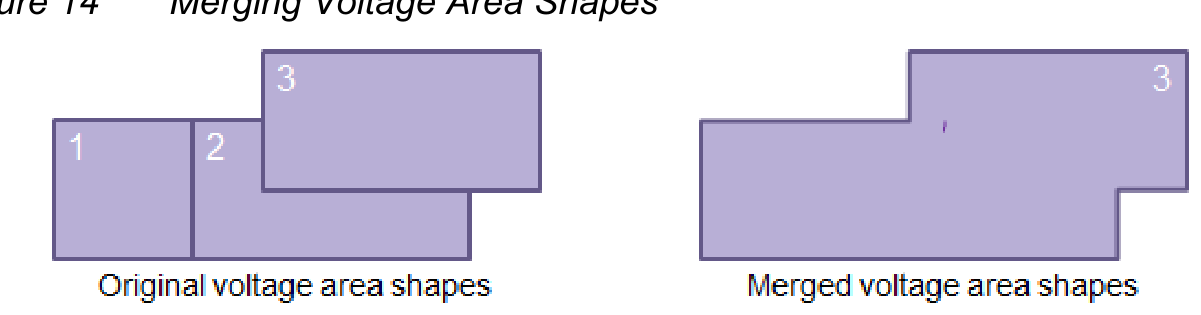
\includegraphics[width=0.92\textwidth,keepaspectratio]{figures/fig-merge-va.png}
\caption{合并电压区域 Shape}
\label{fig:merge-va}
\end{figure}

要用 \cmd{report\_voltage\_areas -verbose} 报告电压区域 shape 的堆叠顺序。

要用 \cmd{set\_voltage\_area\_shape} 修改电压区域 shape 的堆叠顺序，见「修改堆叠顺序」。

\subsubsection{解决重叠电压区域}
\subsubsection*{Resolving Overlapping Voltage Areas}

若来自两个或多个电压区域的 shape 完全或部分重叠，工具用 shape 的堆叠顺序确定各电压区域的有效形状。默认堆叠顺序为定义 shape 的顺序，最后定义的在最上层。工具将重叠区域分配给与顶层 shape 关联的电压区域。与合并同一电压区域内的 shape 不同，解决不同电压区域之间的重叠时，工具不会移除任何 shape；仅解释方式发生变化。

例如，假设要创建如图~\ref{fig:nested-va} 所示的嵌套电压区域。

\begin{figure}[htbp]
\centering
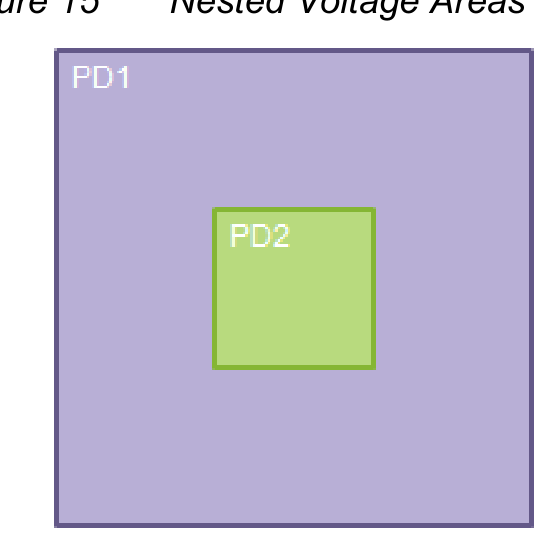
\includegraphics[width=0.45\textwidth,keepaspectratio]{figures/fig-nested-va.png}
\caption{嵌套电压区域}
\label{fig:nested-va}
\end{figure}

要生成这些有效电压区域，必须先指定外层电压区域，再指定内层电压区域，使内层电压区域的 shape 位于上层：
\begin{lstlisting}
fc_shell> create_voltage_area -power_domains PD1 \
   -region { {0 0} {30 30} }
{PD1}
fc_shell> create_voltage_area -power_domains PD2 \
   -region { {10 10} {20 20} }
{PD2}
fc_shell> get_attribute -objects [get_voltage_areas PD2] \
   -name effective_shapes
{{10.0000 10.0000} {20.0000 20.0000}}
fc_shell> get_attribute -objects [get_voltage_areas PD1] \
   -name effective_shapes
{{0.0000 0.0000} {10.0000 0.0000} {10.0000 20.0000} {20.0000 20.0000}
 {20.0000 10.0000} {10.0000 10.0000} {10.0000 0.0000} {30.0000 0.0000}
 {30.0000 30.0000} {0.0000 30.0000}}
\end{lstlisting}

若先指定内层电压区域，则外层电压区域的 shape 在上层并遮蔽内层电压区域，因而被工具忽略，如下例：
\begin{lstlisting}
fc_shell> create_voltage_area -power_domains PD2 \
   -region { {10 10} {20 20} }
{PD2}
fc_shell> create_voltage_area -power_domains PD1 \
   -region { {0 0} {30 30} }
{PD1}
fc_shell> get_attribute -objects [get_voltage_areas PD2] \
   -name effective_shapes
fc_shell> get_attribute -objects [get_voltage_areas PD1] \
   -name effective_shapes
{{0.0000 0.0000} {30.0000 30.0000}}
\end{lstlisting}

要用 \cmd{report\_voltage\_areas -verbose} 报告堆叠顺序；用 \cmd{set\_voltage\_area\_shape} 修改堆叠顺序，见「修改堆叠顺序」。

\subsubsection{修改堆叠顺序}
\subsubsection*{Modifying the Stacking Order}

可用 \cmd{set\_voltage\_area\_shape} 修改电压区域 shape 的堆叠顺序：
\begin{itemize}
  \item \opt{-raise}：将 shape 上移一位
  \item \opt{-lower}：将 shape 下移一位
  \item \opt{-top}：将 shape 移到最顶层
  \item \opt{-bottom}：将 shape 移到最底层
  \item \opt{-above}：将 shape 移到另一 shape 正上方
  \item \opt{-below}：将 shape 移到另一 shape 正下方
\end{itemize}

\subsubsection{定义 Guard Band}
\subsubsection*{Defining Guard Bands}

Guard band 定义环绕电压区域的硬 keepout 边距，其中不能放置任何单元（包括电平移位单元与隔离单元）。Guard band 保证不同电压区域中的单元彼此分离，使电源规划不会引入短路。

默认电压区域没有 guard band。要用 \cmd{create\_voltage\_area} 或 \cmd{create\_voltage\_area\_shape} 的 \opt{-guard\_band}，为 \opt{-region} 中每个 shape 指定水平与垂直 guard band 宽度。水平 guard band 宽度适用于电压区域的全部垂直边；垂直 guard band 宽度适用于全部水平边。

\begin{noteBox}
若同时使用 \opt{-merge\_regions}，必须为合并后的每个不相交 shape 指定 guard band 宽度。通常仅在待合并的全部 shape 邻接或重叠因而合并为单个 shape 时使用该选项。
\end{noteBox}

电压区域 shape 的有效边界包含其 guard band；但其有效可布局面积不包含 guard band。

例如，图~\ref{fig:va-guard} 显示由下列命令定义的 PD1 电压区域周围的 guard band：
\begin{lstlisting}
fc_shell> create_voltage_area -power_domains PD1 \
  -region {{0 0} {30 0} {30 10} {40 10} {40 30} {20 30} {20 25} {0 25}} \
  -guard_band { {3 1} }
\end{lstlisting}

\begin{figure}[htbp]
\centering
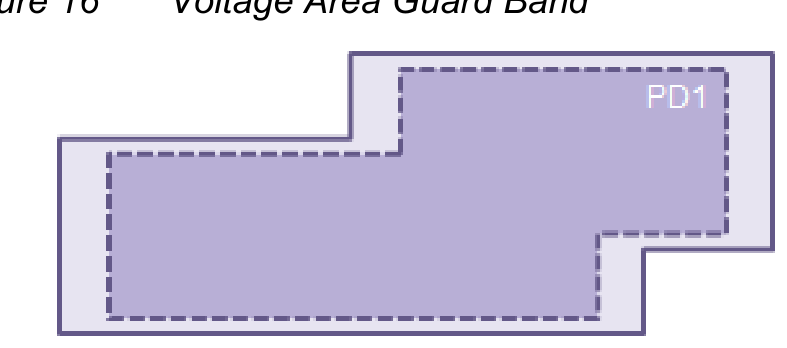
\includegraphics[width=0.92\textwidth,keepaspectratio]{figures/fig-va-guard.png}
\caption{电压区域 Guard Band}
\label{fig:va-guard}
\end{figure}

对同一电压区域关联的邻接或重叠 shape，工具按「合并电压区域 Shape」所述合并 shape，再将顶层 shape 定义的 guard band 应用到合并后的 shape。

例如，假设对图~\ref{fig:merge-va} 右侧所示的电压区域 shape 用下列命令定义 guard band：
\begin{lstlisting}
fc_shell> create_voltage_area -power_domains {PD1} \
   -region { {{0 0} {10 10}} {{10 0} {30 10}} {{15 5} {35 15}} } \
   -guard_band { {1 1} {3 3} {3 1} }
{PD1}
\end{lstlisting}

此时有效 guard band 与图~\ref{fig:va-guard} 所示相同，即合并后 shape 所定义的 guard band。

对不同电压区域关联的重叠 shape，工具用有效边界按「解决重叠电压区域」所述解决 shape。顶层 shape 保留其布局面积与 guard band；较低层 shape 的有效布局面积与 guard band 不包含重叠区域。注意：若邻接 shape 带有 guard band，由于有效边界包含 guard band，它们不再邻接而是重叠。

例如，假设对图~\ref{fig:nested-va} 所示电压区域用下列命令定义 guard band：
\begin{lstlisting}
fc_shell> create_voltage_area -power_domains PD1 \
   -region {{0 0} {30 30}} -guard_band { {2 2} }
{PD1}
fc_shell> create_voltage_area -power_domains PD2 \
   -region {{10 10} {20 20}} -guard_band { {2 2} }
{PD2}
\end{lstlisting}

此时 PD1 的有效布局面积会因 PD2 的有效边界（含其 guard band）而减小，如图~\ref{fig:eff-bound}。

\begin{figure}[htbp]
\centering
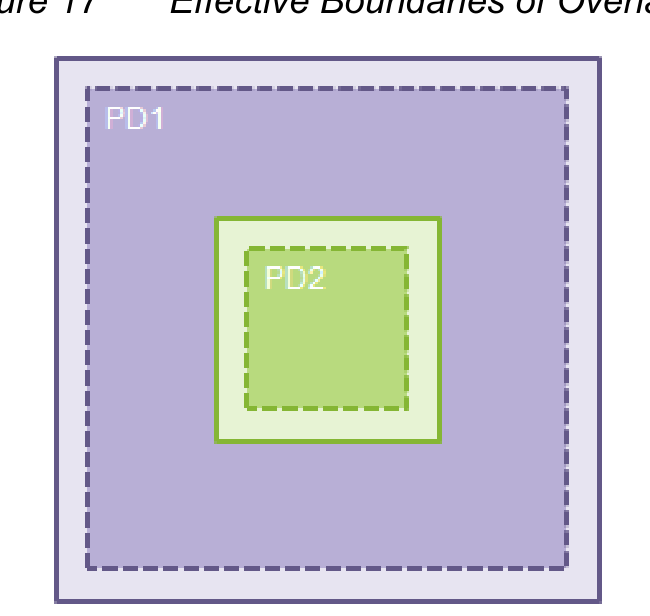
\includegraphics[width=0.45\textwidth,keepaspectratio]{figures/fig-eff-bound.png}
\caption{重叠电压区域的有效边界}
\label{fig:eff-bound}
\end{figure}

\subsubsection{定义 Gas Station}
\subsubsection*{Defining Gas Stations}

Gas station 是为尽量减少在物理 feedthrough 路径上使用双轨（dual-rail）缓冲器而创建的小型电压区域。Gas station 中仅允许单轨中继器，且仅优化步骤可向 gas station 添加单元。

在设计规划阶段用 \cmd{create\_voltage\_area} 创建 gas station。工具会自动识别 gas station，并在绕线迂回代价与使用双轨单元代价之间权衡以使用它们。

用 \cmd{create\_voltage\_area} 的 \opt{-nwell} 与 \opt{-pwell} 为电压区域指定 n-well 与 p-well 供电网。为 gas station 电压区域定义 well 供电可为不同设计风格使用 gas station 提供灵活性。若未对这些选项赋值，则假定 well bias 与域供电值相同。

\cmd{report\_voltage\_areas} 会列出 n-well 与 p-well 供电网，无论是否显式设置。

\subsubsection{查询电压区域}
\subsubsection*{Querying Voltage Areas}

可查询关于电压区域的下列信息：
\begin{itemize}
  \item 当前 block 中的电压区域：用 \cmd{get\_voltage\_areas} 创建当前 block 中电压区域的集合（含默认电压区域）。
  \item 电压区域的详细信息：用 \cmd{report\_voltage\_areas} 显示详细信息（含默认电压区域）。要用 \opt{-verbose} 包含构成各电压区域的 shape 信息。
  \item 电压区域的有效布局面积：查询电压区域的 \appopt{effective\_shapes} 属性。
  \item 电压区域的有效 guard band：查询电压区域的 \appopt{effective\_guard\_band\_boundaries} 属性。也可对单个电压区域 shape 查询该属性。
\end{itemize}

\subsubsection{修改电压区域}
\subsubsection*{Modifying Voltage Areas}

创建电压区域后，可做下列修改：
\begin{itemize}
  \item 更改与电压区域关联的电源域：对 \cmd{set\_voltage\_area} 使用 \opt{-add\_power\_domains} 与 \opt{-remove\_power\_domains}。
  \item 更改电压区域名称：对 \cmd{set\_voltage\_area} 使用 \opt{-name}。
  \item 更改电压区域 region：用 \cmd{create\_voltage\_area\_shape} 添加 shape；用 \cmd{remove\_voltage\_area\_shapes} 移除 shape。
\end{itemize}

\subsubsection{控制电压区域中的物理 Feedthrough Net}
\subsubsection*{Controlling Physical-Feedthrough Nets in Voltage Areas}

若 net 的一个或多个段位于某电压区域的逻辑层次中，则该 net 对该电压区域为 native。若 net 必须在物理上布线经过非 native 电压区域，则它是该电压区域的物理 feedthrough net，如下图所示。

\begin{figure}[htbp]
\centering
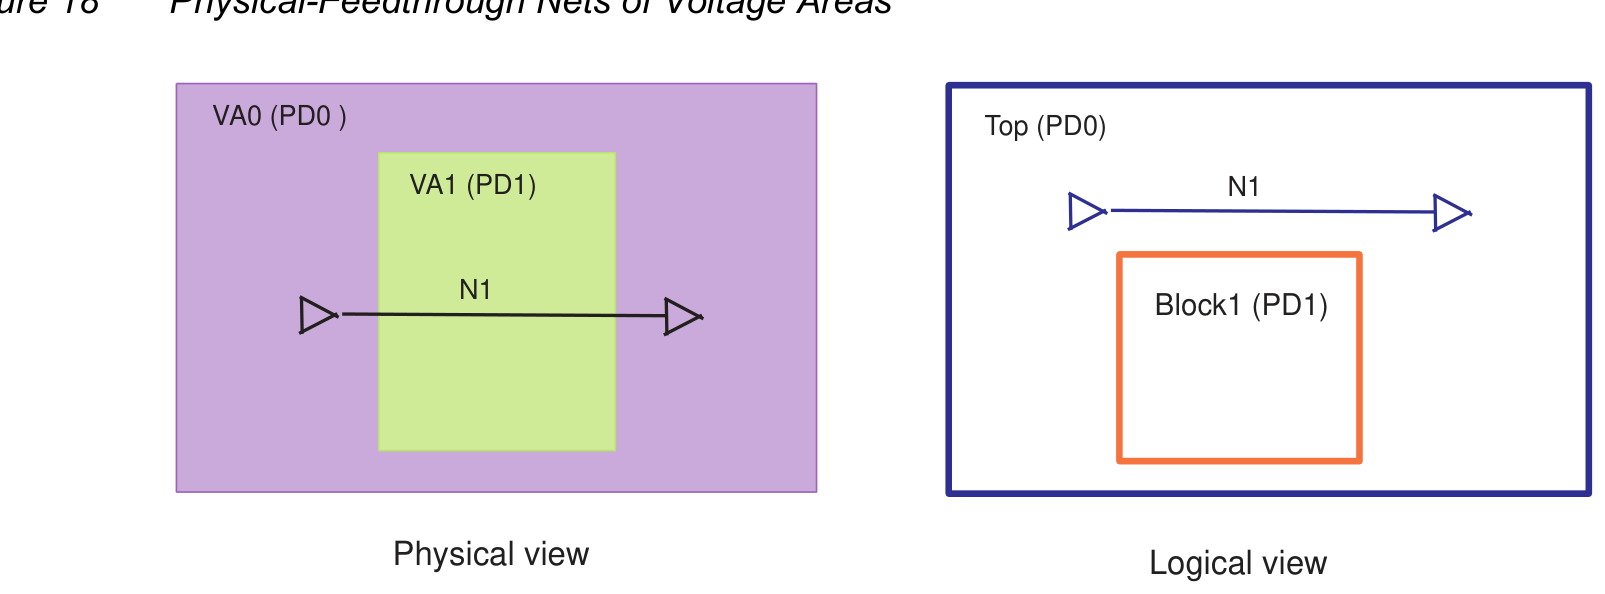
\includegraphics[width=0.92\textwidth,keepaspectratio]{figures/fig-phys-ft.png}
\caption{电压区域的物理 Feedthrough Net}
\label{fig:phys-ft}
\end{figure}

默认允许电压区域中存在物理 feedthrough net。要禁止某电压区域中的物理 feedthrough net，用 \cmd{create\_voltage\_area\_rule -allow\_pass\_through false} 定义电压区域规则，例如：
\begin{lstlisting}
fc_shell> create_voltage_area_rule -allow_pass_through false \
   -name VA1_rule -voltage_areas VA1
\end{lstlisting}

有此规则时，N1 net 会绕开 VA1 电压区域，如图~\ref{fig:phys-ft-off}。

\begin{figure}[htbp]
\centering
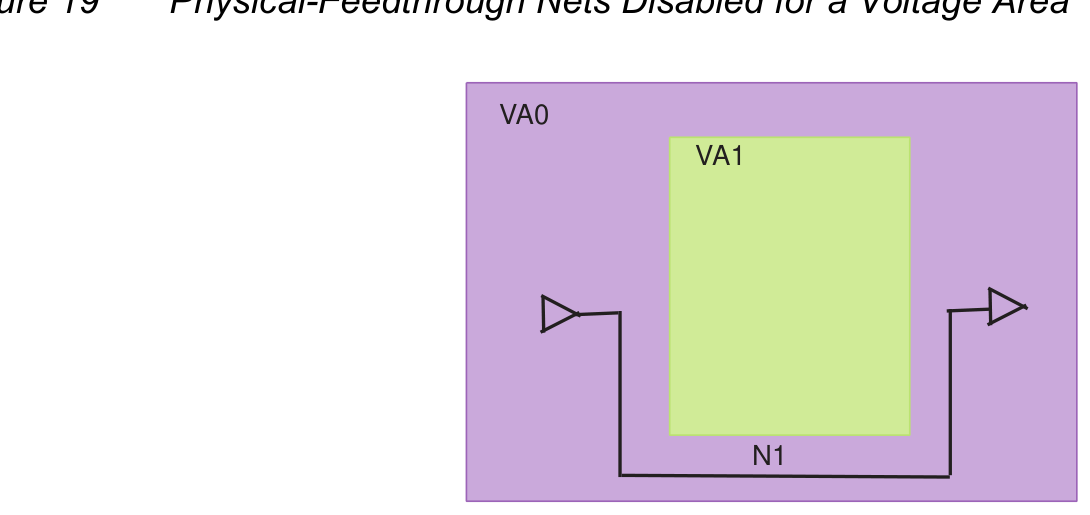
\includegraphics[width=0.92\textwidth,keepaspectratio]{figures/fig-phys-ft-off.png}
\caption{对电压区域禁用物理 Feedthrough Net}
\label{fig:phys-ft-off}
\end{figure}

默认情况下，优化不会在电压区域的物理 feedthrough net 上插入缓冲器。在物理 feedthrough net 上插入缓冲器可能导致缓冲器的逻辑视图与物理视图不匹配。工具通过支持下列优化类型来解决此类不匹配：
\begin{itemize}
  \item \textbf{物理 feedthrough 缓冲（Physical-feedthrough buffering）}\\
    期间工具会：
    \begin{enumerate}
      \item 在其驱动或负载的逻辑层次中插入缓冲器，并用 power-domain-on-instance（PDOI）约束将非 native 电压区域的电源域应用到该缓冲器；
      \item 将缓冲器放在非 native 电压区域内。
    \end{enumerate}
    要允许物理 feedthrough 缓冲，使用 \cmd{create\_voltage\_area\_rule -allow\_physical\_feedthrough true}，例如：
\begin{lstlisting}
fc_shell> create_voltage_area_rule \
   -allow_physical_feedthrough true \
   -name VA1_rule -voltage_areas VA1
\end{lstlisting}

  \item \textbf{逻辑 feedthrough 缓冲（Logical-feedthrough buffering）}\\
    期间工具会：
    \begin{enumerate}
      \item 在与非 native 电压区域对应的逻辑层次中添加缓冲器；
      \item 将缓冲器放在非 native 电压区域内。
    \end{enumerate}
    要允许逻辑 feedthrough 缓冲，使用 \cmd{create\_voltage\_area\_rule -allow\_logical\_feedthrough true}。要用 \opt{-include\_logical\_feedthrough\_hierarchy} 或 \opt{-exclude\_logical\_feedthrough\_hierarchy} 分别指定允许或不允许 feedthrough 缓冲器的逻辑层次。

    下例为 VA1 启用逻辑 feedthrough 缓冲，并将 feedthrough 缓冲器限制为仅 U1 与 U2 层次单元：
\begin{lstlisting}
fc_shell> create_voltage_area_rule \
   -allow_logical_feedthrough true \
   -include_logical_feedthrough_hierarchy {U1 U2}\
   -name VA1_rule -voltage_areas VA1
\end{lstlisting}

    下例为 VA2 启用逻辑 feedthrough 缓冲，并排除 U3 层次单元：
\begin{lstlisting}
fc_shell> create_voltage_area_rule \
   -allow_logical_feedthrough true \
   -exclude_logical_feedthrough_hierarchy {U3}\
   -name VA2_rule -voltage_areas VA2
\end{lstlisting}

\begin{noteBox}
要向下层 block 添加逻辑 feedthrough 缓冲器，工具必须为该 block 添加新的边界 port。因此，用 \cmd{set\_freeze\_ports} 冻结 block 边界会阻止工具向该 block 添加逻辑 feedthrough 缓冲器。
\end{noteBox}
\end{itemize}

\begin{figure}[htbp]
\centering
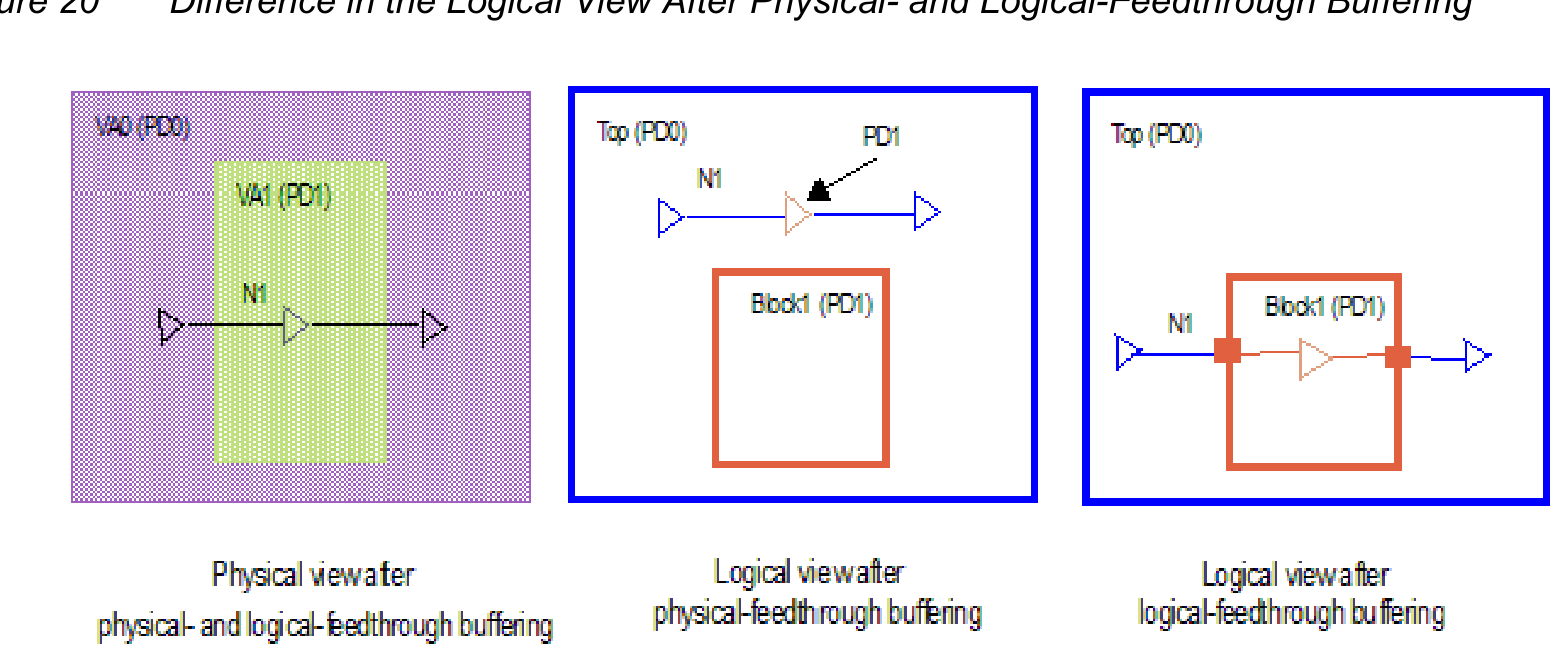
\includegraphics[width=0.92\textwidth,keepaspectratio]{figures/fig-ft-buf-diff.png}
\caption{物理与逻辑 Feedthrough 缓冲后逻辑视图的差异}
\label{fig:ft-buf-diff}
\end{figure}

要用 \cmd{create\_voltage\_area\_rule} 配合 \opt{-default\_rule} 创建适用于所有尚无特定规则的电压区域的默认规则，例如：
\begin{lstlisting}
fc_shell> create_voltage_area_rule -default_rule \
   -allow_physical_feedthrough true
\end{lstlisting}

若某电压区域既无特定规则也无默认规则，则该电压区域的 feedthrough 缓冲由 \appopt{opt.common.allow\_physical\_feedthrough} 应用选项控制。

要用 \cmd{report\_voltage\_area\_rules} 报告电压区域规则；用 \cmd{remove\_voltage\_area\_rules} 移除规则。

\subsubsection{移除电压区域}
\subsubsection*{Removing Voltage Areas}

要用 \cmd{remove\_voltage\_areas} 从 block 移除电压区域。要用 \opt{-all} 移除全部电压区域；要移除特定电压区域，指定电压区域名称。

\subsection{插入多电压单元}
\subsubsection*{Inserting Multivoltage Cells}

多电压设计在电源域接口处需要特殊的多电压单元，例如电平移位单元与隔离单元。电平移位单元用于工作在不同电压电平的电源域之间；隔离单元用于处于不同状态（关断相对 always-on 或上电）的电源域之间。通常多电压单元在逻辑综合期间插入；也可在 Fusion Compiler 中插入。

\subsubsection{插入电平移位单元}
\subsubsection*{Inserting Level Shifters}

电平移位单元作为工作在不同电压电平的电源域之间的接口，确保驱动的输出跳变能使接收单元切换，即使接收端工作在不同电压电平。

\begin{noteBox}
若 block 使用 Design Compiler 综合，自动电平移位插入作为 \cmd{compile\_ultra} 命令的一部分完成。
\end{noteBox}

要在当前 block 中插入电平移位单元，使用 \cmd{create\_mv\_cells}。工具按 UPF 规范中定义的单元映射与策略插入电平移位单元。插入时，工具在电平移位单元上设置 \appopt{size\_only} 属性，并在 port 到电平移位单元的 net 上设置 \appopt{dont\_touch} 属性。

默认情况下，命令仅从 generic library 插入单元。若对 \cmd{create\_mv\_cells} 使用 \opt{-mapped}，则仅从用户提供的逻辑库插入单元；若无合适单元则报错。

若工具未插入电平移位单元，可用 \cmd{analyze\_mv\_design -level\_shifter} 获取更多信息。若用 \opt{-through} 指定 net 或 pin，报告会列出该 net 或 pin 驱动端与负载端的电源域及相关供电，以及说明为何未插入电平移位单元的错误消息。报告包含针对特定插入点的错误，以及适用于经 \opt{-through} 指定的 net 或 pin 整条路径的错误。

\subsubsection{插入隔离单元}
\subsubsection*{Inserting Isolation Cells}

隔离单元用于有选择地关断电源域电压接口的输入侧；它们不进行电平移位。隔离单元应在 RTL 级例化，以避免形式验证错误。也可使用 Fusion Compiler 插入。

要在当前 block 中插入隔离单元，使用 \cmd{create\_mv\_cells}。工具按 UPF 规范中定义的单元映射与策略插入隔离单元。插入时，工具在隔离单元上设置 \appopt{size\_only} 属性，并在 port 到隔离单元的 net 上设置 \appopt{dont\_touch} 属性。

默认情况下，命令仅从 generic library 插入单元。若对 \cmd{create\_mv\_cells} 使用 \opt{-mapped}，则仅从用户提供的逻辑库插入单元；若无合适单元则发出错误消息。

\subsubsection{将功耗策略与已有多电压单元关联}
\subsubsection*{Associating Power Strategies With Existing Multivoltage Cells}

运行 \cmd{associate\_mv\_cells} 或 \cmd{commit\_upf} 时，Fusion Compiler 会自动将功耗策略与已有多电压单元关联。若自动关联不正确，可用 \cmd{set\_power\_strategy\_attribute} 手动修改关联。要用 \cmd{get\_power\_strategies} 确定某电源域的功耗策略。

\subsection{控制多电压单元的布局}
\subsubsection*{Controlling the Placement of Multivoltage Cells}

连接多电压单元（如电平移位单元或隔离单元）到另一电压区域中至少一个单元的 net，称为多电压 net。要缩短多电压 net 长度，将 \appopt{place.coarse.enable\_advanced\_mv\_cell\_placement} 设为 \texttt{true}，以启用高级多电压单元布局。

启用后，工具通过将多电压单元放得更靠近电压区域边界来缩短多电压 net。为优化多电压 net，工具使用双轨缓冲器。缩短多电压 net 可减少优化期间使用的双轨缓冲器数量，并防止因缺乏双轨缓冲器而导致多电压 net 未优化。

\subsection{启用多电压 Net 的改进缓冲}
\subsubsection*{Enabling Improved Buffering for Multivoltage Nets}

多电压 net 是在逻辑或物理上跨越多个电压区域的 net。可将 \appopt{opt.buffering.enable\_hierarchy\_mapping} 设为 \texttt{true}，以在布线前优化期间对这类 net 修复逻辑 DRC 违例时启用改进的缓冲技术。

该应用选项影响 \cmd{place\_opt} 与 \cmd{clock\_opt}。启用后可减少用于修复逻辑 DRC 违例的缓冲器数量，但可能略微增加总负松弛（total negative slack）或 hold 违例数。

\subsection{分析多电压信息}
\subsubsection*{Analyzing Multivoltage Information}

要用 \cmd{check\_mv\_design} 确保设计无多电压设计违例。

可用 \cmd{check\_mv\_design} 限制要检查的规则类型。例如，\opt{-isolation} 指定检查隔离策略与隔离单元规则；\opt{-pg\_pin} 指定检查与 PG pin 相关的规则。

要用表~\ref{tab:mv-rpt} 所列命令报告设计的多电压信息。

\begin{table}[htbp]
\centering
\caption{报告多电压信息的命令}
\label{tab:mv-rpt}
\begin{tabularx}{\textwidth}{@{}l X@{}}
\toprule
\textbf{目的} & \textbf{使用的命令} \\
\midrule
报告多电压信息摘要 & \cmd{report\_mv\_design} \\
报告多电压单元信息 & \cmd{report\_mv\_cells} \\
报告多电压库单元信息 & \cmd{report\_mv\_lib\_cells} \\
报告带多电压约束的路径及相关多电压单元 & \cmd{report\_mv\_path} \\
报告电源域 & \cmd{report\_power\_domains} \\
检查指定电源域是否等价 & \cmd{check\_equivalent\_power\_domains} \\
显示等价电源域列表 & \cmd{get\_equivalent\_power\_domains} \\
报告电压区域 & \cmd{report\_voltage\_areas} \\
\bottomrule
\end{tabularx}
\end{table}

% ============================================================
\section{指定时序约束与设置}
\subsection*{Specifying Timing Constraints and Settings}

时序约束描述设计的时序要求。时序约束的关键部分是准确指定的时钟及其效应（如 latency 与 uncertainty）。指定时钟后，工具自动约束由这些时钟驱动的寄存器之间的路径。但可通过指定时序例外（timing exceptions）改变这些时序路径的默认行为，例如不应分析的路径（false paths）、需要多个时钟周期的路径（multicycle paths）等。此外，可通过为输入与输出 port 指定 input/output delay 来约束边界时序路径。

Fusion Compiler 使用片上偏差（on-chip variation，OCV）模式进行时序分析，以建模芯片上工作条件变化的影响。该模式执行保守的时序分析，允许最小与最大延迟同时作用于不同路径。对 setup 检查，发射时钟路径与数据路径使用最大延迟，捕获时钟路径使用最小延迟；对 hold 检查，发射时钟路径与数据路径使用最小延迟，捕获时钟路径使用最大延迟。

一个 block 可能在多种条件（如不同温度与电压）下工作，并可能处于多种功能模式。时序分析中，每组条件由一个 \textbf{corner} 表示，每个功能模式由一个 \textbf{mode} 表示。\textbf{scenario} 是用于时序分析与优化的 corner 与 mode 的组合。开始处理 block 之前，必须定义用于该 block 的 mode、corner 与 scenario，以及延迟计算模型与所用布线层。所指定的布线层信息用于时序分析期间的 RC 估计。

详细信息见：
\begin{itemize}
  \item 时钟与时钟效应：\textit{Fusion Compiler Timing Analysis User Guide} 中的 ``Defining Clocks''；
  \item 时序路径例外与边界路径约束：同上指南中的 ``Constraining Timing Paths''；
  \item Mode、corner 与 scenario：同上指南中的 ``Defining Modes, Corners, and Scenarios''；
  \item 工作条件与 OCV 相关设置：同上指南中的 ``Specifying Operating Conditions''；
  \item RC 估计与提取的寄生信息：同上指南中的 ``Performing Parasitic Extraction''。
\end{itemize}

% ============================================================
\section{指定逻辑设计规则约束}
\subsection*{Specifying Logical Design Rule Constraints}

最小电容、最大电容与最大 transition 是设计必须满足才能按预期工作的逻辑设计规则约束。它们是在逻辑库中指定的工艺相关限制。但可用表~\ref{tab:drc-cmd} 中的约束命令指定更严格的设计规则约束。

优化期间，Fusion Compiler 会设法满足设计规则约束，即使这意味着违反时序、功耗与面积等优化约束——这些设计规则约束具有更高优先级。优化后，可用表~\ref{tab:drc-cmd} 中的报告命令识别 block 中的设计规则约束违例。

\begin{table}[htbp]
\centering
\caption{设计规则相关命令}
\label{tab:drc-cmd}
\begin{tabularx}{\textwidth}{@{}X l@{}}
\toprule
\textbf{目的} & \textbf{使用的命令} \\
\midrule
为输入 port、库单元 pin、叶子单元 pin、时钟或 block 指定允许的最小电容 & \cmd{set\_min\_capacitance} \\
为输入 port、库单元 pin、叶子单元 pin、时钟或 block 指定允许的最大电容 & \cmd{set\_max\_capacitance} \\
为输入 port、库单元 pin、叶子单元 pin、时钟或 block 指定允许的最大信号 transition 时间 & \cmd{set\_max\_transition} \\
移除用户指定的最小电容约束 & \cmd{remove\_min\_capacitance} \\
移除用户指定的最大电容约束 & \cmd{remove\_max\_capacitance} \\
移除用户指定的最大 transition 约束 & \cmd{remove\_max\_transition} \\
报告最小电容约束违例 & \cmd{report\_constraints -min\_capacitance} \\
报告最大电容约束违例 & \cmd{report\_constraints -max\_capacitance} \\
报告最大 transition 约束违例 & \cmd{report\_constraints -max\_transition} \\
\bottomrule
\end{tabularx}
\end{table}

\begin{noteBox}
Fusion Compiler 不遵从最大 fanout 设计规则约束。但可用 \appopt{opt.common.max\_fanout} 应用选项为 block 中的数据路径指定最大 fanout。这是软优化约束。优化期间工具会设法确保数据路径单元驱动的扇出不超过指定的最大 fanout。
\end{noteBox}

% ============================================================
\section{指定时钟门控约束}
\subsection*{Specifying Clock Gating Constraints}

默认情况下，工具在执行 \cmd{analyze} 与 \cmd{elaborate} 期间识别已有的时钟门控单元。在 compile 期间，若你未指定任何时钟门控约束，工具会在叶子级再插入一级时钟门控单元，并用默认时钟门控设置实现时钟门控逻辑。不能禁用时钟门控。

在设置时钟门控约束之前，先将设计与库载入内存，然后用下列命令设置约束：

\begin{itemize}
  \item \cmd{set\_clock\_gate\_style}\\
    要选择集成时钟门控单元的类型，指定下列选项：

\begin{table}[htbp]
\centering
\caption{\cmd{set\_clock\_gate\_style} 选项}
\label{tab:fc-cg-style}
\begin{tabularx}{\textwidth}{@{}l X@{}}
\toprule
\textbf{选项} & \textbf{说明} \\
\midrule
\opt{-test\_point} & 指定相对集成时钟门控单元的测试控制位置。有效取值为 \texttt{none}、\texttt{before} 与 \texttt{after}。 \\
\opt{-observation\_output} & 指定观察输出 pin。 \\
\opt{-target} & 指定要被时钟门控的目标时序元件。有效取值为 \texttt{pos\_edge\_flip\_flop} 与 \texttt{neg\_edge\_flip\_flop}。 \\
\opt{-objects} & 指定时钟门控所作用的对象。 \\
\bottomrule
\end{tabularx}
\end{table}

  \item \cmd{set\_clock\_gating\_options}\\
    要定义所插入时钟门控单元的网表结构，指定下列选项：

\begin{table}[htbp]
\centering
\caption{\cmd{set\_clock\_gating\_options} 选项}
\label{tab:fc-cg-options}
\begin{tabularx}{\textwidth}{@{}l X@{}}
\toprule
\textbf{选项} & \textbf{说明} \\
\midrule
\texttt{minimum\_bitwidth} & 指定一起门控的最小位数。默认值为 3。 \\
\texttt{max\_fanout} & 指定同一时钟门控单元所门控的最大单元数。默认值为无穷大（infinite）。 \\
\bottomrule
\end{tabularx}
\end{table}

  \item \cmd{set\_clock\_gating\_objects}\\
    要控制指定对象的时钟门控，并覆盖 compile 期间设置的默认时钟门控行为，指定下列选项。对象可以是层次单元、寄存器、电源域或模块。

\begin{table}[htbp]
\centering
\caption{\cmd{set\_clock\_gating\_objects} 选项}
\label{tab:fc-cg-objects}
\begin{tabularx}{\textwidth}{@{}l X@{}}
\toprule
\textbf{选项} & \textbf{说明} \\
\midrule
\opt{-include} & 指定按时钟门控风格与时钟门控选项进行门控的对象列表。 \\
\opt{-exclude} & 指定从时钟门控中排除的对象列表。 \\
\opt{-clear} & 指定移除给定对象列表的全部时钟门控包含或排除设置。 \\
\opt{-reset} & 指定移除先前由 \cmd{set\_clock\_gating\_objects} 设置的全部条件。 \\
\bottomrule
\end{tabularx}
\end{table}

  \item 默认值\\
    时钟门控优化期间，工具使用下列设置默认值：

\begin{table}[htbp]
\centering
\caption{时钟门控默认设置}
\label{tab:fc-cg-defaults}
\begin{tabularx}{\textwidth}{@{}l X@{}}
\toprule
\textbf{设置} & \textbf{默认值} \\
\midrule
最大扇出（Maximum fanout） & 无穷大（Infinite） \\
最小位宽（Minimum bit-width） & 3 \\
时钟门控单元（Clock-gating cell） & 对正沿与负沿触发触发器均使用基于锁存器（latch-based）的单元。若仅有一种类型可用，工具在时钟门控单元两侧插入反相器。 \\
\bottomrule
\end{tabularx}
\end{table}
\end{itemize}

\begin{seeAlsoBox}
更多信息见 Setting Up Clock Gating。
\end{seeAlsoBox}


% ============================================================
\section{控制时钟门控延迟}
\subsection*{Controlling Clock-Gate Latencies}

综合期间，Fusion Compiler 假定时钟为理想时钟。理想时钟在时钟网络上不产生延迟。作出该假定是因为真实时钟网络延迟要到时钟树综合之后才可知。实际上时钟并非理想，时钟网络上存在非零延迟。对带时钟门控的设计，寄存器处的时钟网络延迟与时钟门控单元处的时钟网络延迟不同。寄存器与时钟门控单元之间的时钟网络延迟差异，会使时钟门控单元使能输入处的 setup 条件约束更紧。

工具可通过下列方式获得时钟门控延迟：
\begin{itemize}
  \item \textbf{集成延迟估计（Integrated latency estimation）}\\
    默认情况下，工具在整个流程中估计并更新时钟门控延迟。估计的时钟延迟比用户指定的时钟延迟更准确。
  \item \textbf{用户指定延迟（User-specified latency）}\\
    可对特定实例禁用集成延迟估计，并手动指定延迟值。
\end{itemize}

\subsection{集成时钟门控延迟估计}
\subsubsection*{Integrated Clock-Gate Latency Estimation}

默认情况下，工具在整个 \cmd{place\_opt} 命令流程中估计并更新时钟门控延迟。这确保在时钟树综合之前、时钟仍为理想时，工具在数据路径优化与 useful-skew 优化中使用准确的时钟门控延迟。

若计划对设计执行结构性多源时钟树综合（structural multisource clock tree synthesis），请将 \appopt{opt.clock\_latency\_estimation.estimate\_smscts\_subtrees} 设为 \texttt{true}，以确保工具估计适合结构性多源时钟子树的时钟门控延迟。

为提高估计时钟门控延迟的准确性，在运行 \cmd{place\_opt} 之前指定时钟树综合设置，包括时钟树缓冲器库单元列表、时钟树反相器库单元列表以及时钟非默认布线规则（NDR）。

估计的时钟延迟比用户指定的更准确。此外，工具在布局与多比特 banking 等步骤之后会更新估计的时钟延迟，而用户指定的延迟是静态值。

要阻止工具估计特定时钟门控的延迟，用 \cmd{set\_attribute} 在其时钟 pin 上设置 \appopt{dont\_estimate\_clock\_latency} 属性，例如：
\begin{lstlisting}
fc_shell> set_attribute \
   [get_pins {ICG21/CK}] dont_estimate_clock_latency true
\end{lstlisting}

为获得最佳结果，请勿将下列功能与集成时钟门控延迟估计一起使用：
\begin{itemize}
  \item Trial clock tree synthesis：将 \appopt{place\_opt.flow.trial\_clock\_tree} 设为 \texttt{false} 以禁用。
  \item Clock-gate optimization：将 \appopt{place\_opt.flow.optimize\_icgs} 设为 \texttt{false} 以禁用。
  \item 用户指定延迟：用户指定延迟由 \cmd{set\_clock\_latency}、\cmd{set\_clock\_gate\_latency}、\cmd{set\_clock\_gating\_check -setup} 或 \cmd{set\_path\_margin -setup} 设置。
\end{itemize}

工具不会修改你在时钟门控单元上指定的任何 \cmd{set\_clock\_latency} 约束。工具估计的时钟门控延迟值存储为相对用户指定值的偏移（offset）。可用 \cmd{write\_script -format icc2} 查看偏移值，并在生成输出中查找 \cmd{set\_clock\_latency -offset} 命令。若未设置任何延迟值，报告的偏移等于估计延迟值。

由 \cmd{write\_sdc} 生成的 SDC 文件不会捕获估计的延迟偏移值。

若时钟门控及其被门控寄存器的相对位置在时钟树综合期间不变，延迟估计最准确。要保持集成时钟门控的布局，在时钟树综合之前将 \appopt{cts.compile.enable\_cell\_relocation} 设为 \texttt{auto}，以启用时钟网络单元的自动重定位。

\subsection{用户指定的时钟门控延迟}
\subsubsection*{User-Specified Clock-Gate Latency}

不能禁用通用的集成时钟门控延迟估计；但可通过在时钟门控单元的时钟 pin 上设置 \appopt{dont\_estimate\_clock\_latency} 属性，对特定时钟门控禁用该功能。本节说明如何对这些时钟门控手动指定延迟值。

用 \cmd{set\_clock\_latency} 或 \cmd{set\_clock\_gate\_latency} 指定时钟网络延迟。\cmd{set\_clock\_gate\_latency} 可用于门级与 RTL 设计。

用 \cmd{set\_clock\_gate\_latency} 指定的时钟延迟，在 \cmd{compile\_fusion} 插入时钟门控单元时标注到寄存器。但若在编译后修改时钟门控上的延迟值，必须用 \cmd{apply\_clock\_gate\_latency} 手动将延迟值应用到已有时钟门控单元。

\begin{noteBox}
用 \cmd{set\_clock\_gate\_latency} 修改时钟门控延迟后，若再用 \cmd{compile\_fusion} 编译设计，则不必再用 \cmd{apply\_clock\_gate\_latency} 应用延迟值；工具会在编译期间标注指定值。
\end{noteBox}

要用 \cmd{reset\_clock\_gate\_latency} 移除先前由 \cmd{set\_clock\_gate\_latency} 或 \cmd{apply\_clock\_gate\_latency} 在时钟门控单元上设置的时钟延迟信息。该命令移除指定时钟上的时钟延迟值；若未指定时钟，则移除全部时钟门控单元上的时钟延迟值。

\subsubsection{\texttt{set\_clock\_latency} 命令}
\subsubsection*{The set\_clock\_latency Command}

用 \cmd{set\_clock\_latency} 为特定时钟门控单元指定时钟网络延迟。

在图~\ref{fig:clk-lat-cg} 中，\texttt{lat\_cgtoreg} 是从时钟门控单元时钟 pin 到被门控寄存器时钟 pin 的估计延迟；\texttt{lat\_reg} 是到无时钟门控的寄存器时钟 pin 的估计时钟网络延迟。

\begin{figure}[htbp]
\centering
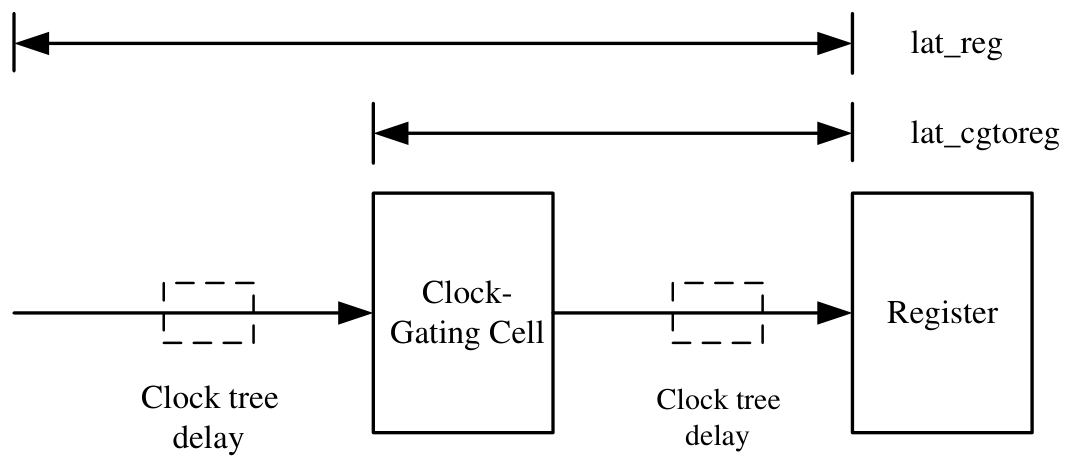
\includegraphics[width=0.92\textwidth,keepaspectratio]{figures/fig-clk-lat-cg.png}
\caption{带时钟门控设计的时钟延迟}
\label{fig:clk-lat-cg}
\end{figure}

对设计中由特定时钟驱动的全部寄存器（有门控或无门控）的时钟 pin，对 \cmd{set\_clock\_latency} 使用 \texttt{lat\_reg} 值。对全部时钟门控单元的时钟 pin，使用 \texttt{lat\_reg} 与 \texttt{lat\_cgtoreg} 之差。由于设置延迟值的目的是计入寄存器与时钟门控单元之间不同的时钟网络延迟，获得合理准确的差值（\texttt{lat\_cgtoreg}）很重要。除非要用这些值处理与时钟门控无关的时钟网络延迟问题，否则绝对值相对次要。

\subsubsection{\texttt{set\_clock\_gate\_latency} 命令}
\subsubsection*{The set\_clock\_gate\_latency Command}

使用 \cmd{compile\_fusion} 时，时钟门控在编译过程中插入。要在工具插入时钟门控单元之前指定时钟网络延迟，使用 \cmd{set\_clock\_gate\_latency}。该命令允许你将时钟门控单元的时钟网络延迟指定为时钟域、时钟门控级数（stage）以及时钟门控单元扇出的函数。你指定的延迟在 \cmd{compile\_fusion} 插入时钟门控单元时标注到这些单元。可用 \cmd{apply\_clock\_gate\_latency} 手动将延迟值标注到设计中已有的时钟门控单元。

\cmd{set\_clock\_gate\_latency} 接受下列参数：
\begin{itemize}
  \item \opt{-clock clock\_list}
  \item \opt{-stage clock\_gate\_stage}
  \item \opt{-fanout\_latency fanout\_list}
\end{itemize}

\texttt{fanout\_list} 是指定扇出范围与延迟减量的元组列表。下例创建三个扇出范围：1 到 5 延迟为 0.5；6--15 为 0.8；16 到无穷大为 0.6。
\begin{lstlisting}
set_clock_gate_latency -stage 1 \
      -fanout_latency {{1-5 0.5} {6-15 0.8} {16-inf 0.6}}
\end{lstlisting}

要为被时钟门控的寄存器指定时钟延迟值，对 \opt{-stage} 使用值 0。由于是为被门控寄存器指定延迟，\opt{-fanout\_latency} 应为 \texttt{1-inf}（1 到无穷大），且延迟为寄存器的绝对时钟延迟值，例如：
\begin{lstlisting}
set_clock_gate_latency -clock CLK -stage 0\
      -fanout_latency {1-inf 1.0}
\end{lstlisting}

若未指定 \opt{-clock}，设置适用于设计中全部时钟。用 \cmd{set\_clock\_latency} 设置的时钟延迟优先级更高，不会被覆盖。

图~\ref{fig:cg-stages} 给出时钟门控级数与扇出示例。

\begin{figure}[htbp]
\centering
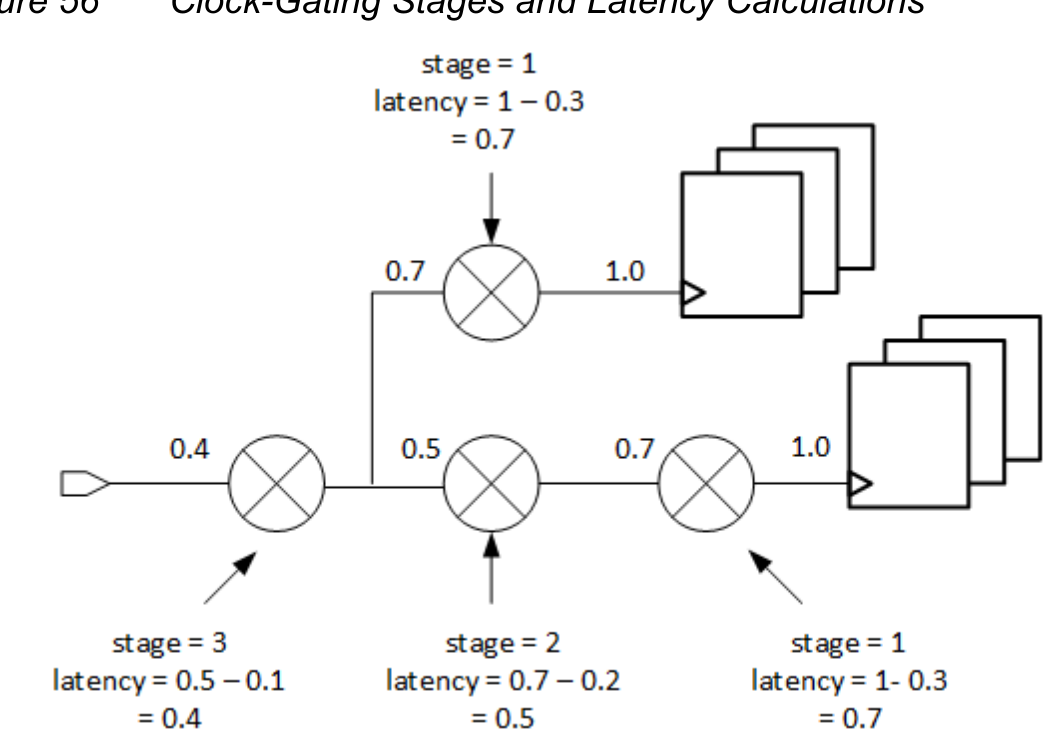
\includegraphics[width=0.70\textwidth,keepaspectratio]{figures/fig-cg-stages.png}
\caption{时钟门控级数与延迟计算}
\label{fig:cg-stages}
\end{figure}

下列命令为图~\ref{fig:cg-stages} 设置延迟值：
\begin{lstlisting}
set_clock_gate_latency -stage 0 -fanout_latency {{1-inf 1.0}}
set_clock_gate_latency -stage 1 -fanout_latency {{1-inf 0.3}}
set_clock_gate_latency -stage 2 -fanout_latency {{1-inf 0.2}}
set_clock_gate_latency -stage 3 -fanout_latency {{1-inf 0.1}}
\end{lstlisting}

图~\ref{fig:lat-fanout} 给出另一扇出与延迟计算示例。

\begin{figure}[htbp]
\centering
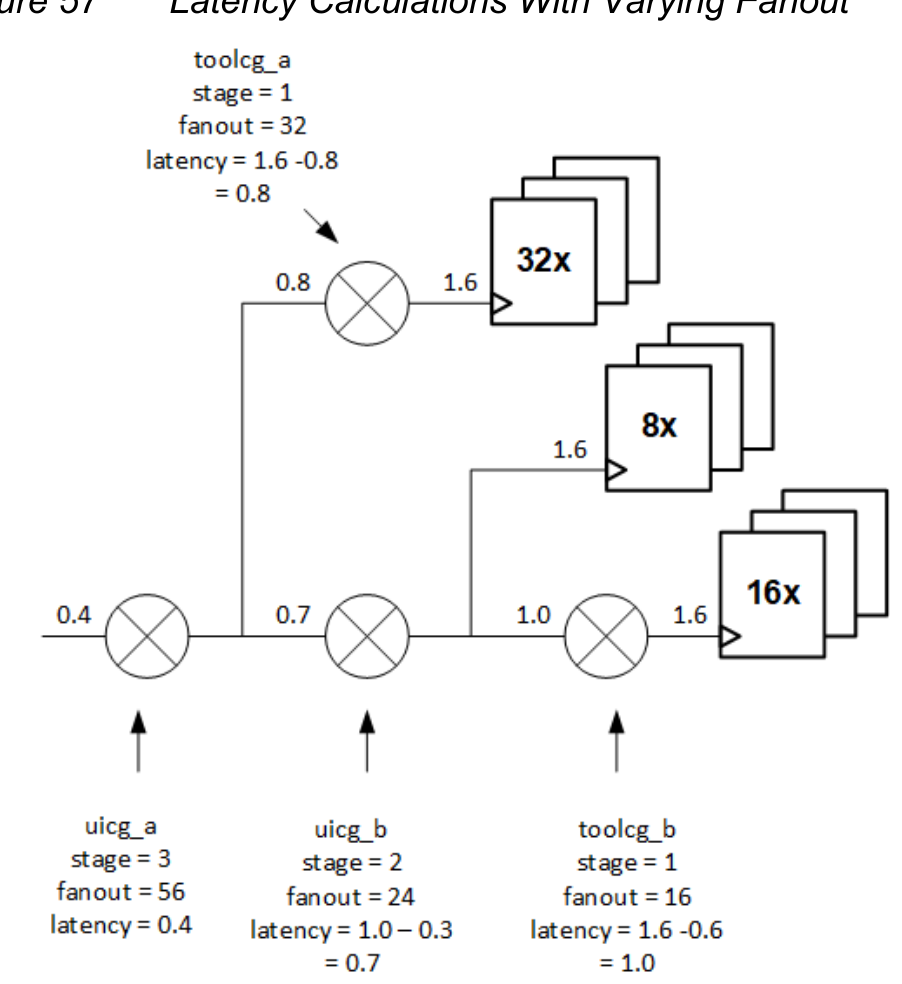
\includegraphics[width=0.55\textwidth,keepaspectratio]{figures/fig-lat-fanout.png}
\caption{变化扇出下的延迟计算}
\label{fig:lat-fanout}
\end{figure}

下列命令为图~\ref{fig:lat-fanout} 指定延迟与扇出：
\begin{lstlisting}
set_clock_gate_latency -stage 0 \
   -fanout_latency {{1-inf 1.6}}
set_clock_gate_latency -stage 1 \
   -fanout_latency {{1-20 0.6} {21-inf 0.8}}
set_clock_gate_latency -stage 2 \
   -fanout_latency {{1-20 0.2} {21-inf 0.3}}
set_clock_gate_latency -stage 3 \
   -fanout_latency {{1-30 0.1} {31-65 0.8} {66-inf 0.18}}
set_clock_latency "0.4" {uicg_a/CK}
\end{lstlisting}

注意：对时钟门控 \texttt{uicg\_a}，用 \cmd{set\_clock\_latency} 赋值为 0.4 的延迟不会被覆盖。

% ============================================================
\section{为布局与合法化指定物理约束}
\subsection*{Specifying Physical Constraints for Placement and Legalization}

布局与合法化期间，floorplan 信息决定单元放置位置。下列主题说明如何指定影响布局与合法化的额外物理约束：
\begin{itemize}
  \item 定义 Keepout Margins
  \item 定义基于区域的布局障碍（Area-Based Placement Blockages）
  \item 定义布局 Bounds（Placement Bounds）
  \item 定义布局吸引（Placement Attractions）
  \item 为合法化定义单元间距约束
\end{itemize}

\subsection{定义 Keepout Margins}
\subsubsection*{Defining Keepout Margins}

Keepout margin 是 block 中固定单元边界周围的区域（如图~\ref{fig:keepout} 阴影部分），其中不放置其他单元。

\begin{figure}[htbp]
\centering
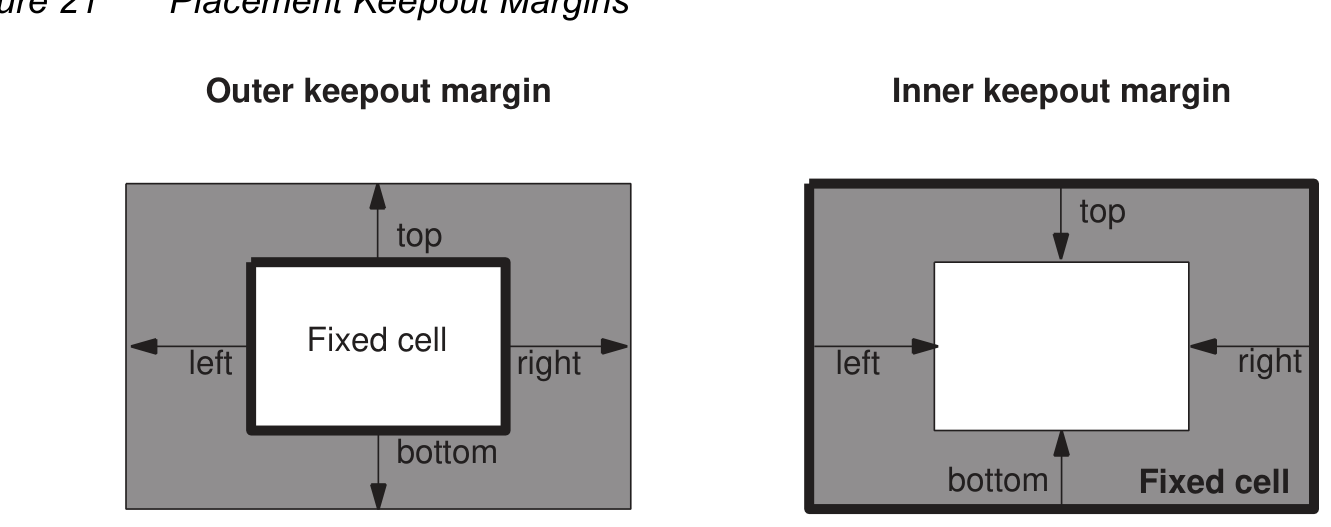
\includegraphics[width=0.92\textwidth,keepaspectratio]{figures/fig-keepout.png}
\caption{布局 Keepout Margins}
\label{fig:keepout}
\end{figure}

\textbf{Outer keepout margin} 是单元边界外的区域；\textbf{inner keepout margin} 是单元边界内的区域。固定单元各侧 keepout margin 的宽度可以相同或不同，取决于如何定义。此外，keepout margin 可定义为 hard 或 soft。将单元排除在此类区域之外可避免拥塞与 net 绕行，并获得更好的 QoR。

要用 \cmd{create\_keepout\_margin} 定义 keepout margin。默认创建 hard keepout margin；要创建 soft keepout margin，使用 \opt{-type soft}。

\subsubsection{定义 Outer Keepout Margin}
\subsubsection*{Defining an Outer Keepout Margin}

可在硬宏、层次单元或叶子单元上定义 outer keepout margin。定义时，可显式指定 keepout 距离；对硬宏，也可让工具根据宏 pin 数量推导 keepout 距离。

要显式指定 outer keepout margin，用 \opt{-outer} 为各侧指定边距。按 \texttt{\{lx by rx ty\}} 格式指定左、下、右、上边距。值为 0 表示该侧无 keepout margin。

例如，为名为 \texttt{my\_macro} 的宏创建各侧边距为 10 的 hard outer keepout margin：
\begin{lstlisting}
fc_shell> create_keepout_margin -outer {10 10 10 10} my_macro
\end{lstlisting}

要让工具根据硬宏的 pin 数量推导 outer keepout 距离，用 \opt{-tracks\_per\_macro\_pin} 指定 track 与 pin 之比。使用该选项时，工具根据 track 宽度、宏 pin 数量以及指定的 track-to-pin 比计算 keepout margin，该比通常设为接近 0.5 的值。较大值产生较大 keepout margin。推导的 keepout margin 始终为 hard；\opt{-type} 设置被忽略。推导的边距受 \opt{-min\_padding\_per\_macro} 与 \opt{-max\_padding\_per\_macro} 指定的最小与最大值约束。

例如，以 track-to-pin 比 0.6、最小 keepout 距离 0.1、最大 keepout 距离 0.2 为名为 \texttt{my\_macro} 的宏推导 outer keepout margin：
\begin{lstlisting}
fc_shell> create_keepout_margin -tracks_per_macro_pin 0.6 \
   -min_padding_per_macro 0.1 -max_padding_per_macro 0.2 my_macro
\end{lstlisting}

\subsubsection{定义 Inner Keepout Margin}
\subsubsection*{Defining an Inner Keepout Margin}

可在层次单元上定义 inner keepout margin，但不能在硬宏或叶子单元上定义。定义 inner keepout margin 时必须显式指定 keepout 距离。

要用 \opt{-inner} 为各侧指定边距，格式为 \texttt{\{lx by rx ty\}}。值为 0 表示该侧无 keepout margin。

例如，为名为 \texttt{my\_hcell} 的层次单元创建各侧边距为 10 的 hard inner keepout margin：
\begin{lstlisting}
fc_shell> create_keepout_margin -inner {10 10 10 10} my_hcell
\end{lstlisting}

\subsection{定义基于区域的布局障碍}
\subsubsection*{Defining Area-Based Placement Blockages}

基于区域的布局障碍是矩形区域，其中不能放置单元，或对单元类型或数量加以限制。Fusion Compiler 支持下列类型的基于区域的布局障碍：
\begin{itemize}
  \item \textbf{Hard}：在粗布局、优化与合法化期间阻止在指定区域内放置标准单元与硬宏。
  \item \textbf{Hard macro}：在粗布局、优化与合法化期间阻止在指定区域内放置硬宏。
  \item \textbf{Soft}：在粗布局期间阻止在指定区域内放置标准单元与硬宏，但允许优化与合法化在指定区域内放置单元。
  \item \textbf{Partial}：在粗布局期间限制指定区域内的单元密度，对优化与合法化无影响。
\end{itemize}

要用 \cmd{create\_placement\_blockage} 定义布局障碍。至少须指定布局障碍的坐标。要创建矩形布局障碍，用 \opt{-boundary} 指定矩形左下角与右上角坐标；要创建直角多边形布局障碍，用 \opt{-boundary} 指定多边形坐标。也可通过将边界多边形指定为 \texttt{geo\_mask} 或物理对象集合来创建多个布局障碍。若结果区域解析为多个非连续多边形，命令为每个多边形创建一个布局障碍。

默认情况下，\cmd{create\_placement\_blockage} 创建 hard 布局障碍。要创建其他类型，用 \opt{-type} 指定障碍类型。单次 \cmd{create\_placement\_blockage} 只能创建一种类型的布局障碍。

可用 \opt{-name} 为布局障碍指定名称，以便按名查询或移除。

\subsubsection{定义 Hard 布局障碍}
\subsubsection*{Defining a Hard Placement Blockage}

要定义 hard 布局障碍，指定边界，并可选择指定名称。

例如，在角点为 $(10, 20)$ 与 $(100, 200)$ 的矩形区域内创建 hard 布局障碍：
\begin{lstlisting}
create_placement_blockage -boundary {10 20 100 200}
\end{lstlisting}

\begin{noteBox}
Hard 布局障碍在布局、合法化、优化与时钟树综合期间均被遵从。
\end{noteBox}

Hard 布局障碍也可在 DEF 中定义，如 Example~13。

\begin{lstlisting}
# Example 13: Placement Blockages in DEF
BLOCKAGES 2 ;
  - PLACEMENT
   RECT ( 0 327600 ) ( 652740 327660 ) ;
  - PLACEMENT
   RECT ( 0 327600 ) ( 652740 327660 ) ;
END BLOCKAGES
\end{lstlisting}

\subsubsection{定义 Hard Macro 布局障碍}
\subsubsection*{Defining a Hard Macro Placement Blockage}

要定义 hard macro 障碍，指定边界、类型（\opt{-type hard\_macro}），并可选择指定名称。

例如，定义角点为 $(120, 75)$ 与 $(230, 200)$ 的 hard macro 障碍：
\begin{lstlisting}
create_placement_blockage -boundary {120 75 230 200} \
   -type hard_macro
\end{lstlisting}

\begin{noteBox}
Hard macro 布局障碍在布局、合法化与优化期间被遵从。这是硬宏布局所遵从的唯一布局障碍类型。
\end{noteBox}

\subsubsection{定义 Soft 布局障碍}
\subsubsection*{Defining a Soft Placement Blockage}

要定义 soft 障碍，指定边界、类型（\opt{-type soft}），并可选择指定名称。

例如，定义角点为 $(120, 75)$ 与 $(230, 200)$ 的 soft 障碍：
\begin{lstlisting}
create_placement_blockage -boundary {120 75 230 200} \
   -type soft
\end{lstlisting}

Soft 障碍阻止初始布局在指定区域内放置单元，但允许合法化、优化与时钟树综合这样做。然而，在布局与优化之后的后续增量布局中，工具可将合法化、优化与时钟树综合期间添加的单元移出 soft blockage 区域。要防止此行为，使用下列应用选项设置：
\begin{lstlisting}
set_app_options -name place.coarse.enable_enhanced_soft_blockages \
   -value true
\end{lstlisting}

\begin{noteBox}
Soft 布局障碍在布局期间被遵从，但在合法化、优化或时钟树综合期间不被遵从。
\end{noteBox}

\subsubsection{定义 Partial 布局障碍}
\subsubsection*{Defining a Partial Placement Blockage}

要定义 partial 障碍，指定边界、类型（\opt{-type partial}）、障碍百分比（\opt{-blocked\_percentage}），并可选择指定名称。

例如，定义最大允许单元密度为 60\%（blocked percentage 为 40）、角点为 $(10, 20)$ 与 $(100, 200)$ 的 partial 障碍：
\begin{lstlisting}
create_placement_blockage -boundary {10 20 100 200} \
   -type partial -blocked_percentage 40
\end{lstlisting}

要允许无限制使用 partial blockage 区域，将障碍百分比指定为 0（\opt{-blocked\_percentage 0}）。

\begin{noteBox}
Partial 布局障碍在布局期间被遵从，但在合法化、优化或时钟树综合期间不被遵从。
\end{noteBox}

\subsubsection{定义预定义类别的障碍}
\subsubsection*{Define a Blockage of a Predefined Category}

类别障碍（category blockage）是一种特殊的 partial 障碍，用于控制预定义单元类别在 partial blockage 内的布局。

要创建类别障碍：
\begin{enumerate}
  \item 用 \cmd{define\_user\_attribute} 为类别定义用户属性，并用 \cmd{set\_attribute} 将其应用到受影响的单元参考或实例。\\
    要阻止单元放入类别障碍，将属性设为 \texttt{true}；要允许放入，设为 \texttt{false}。\\
    定义与应用属性时遵守下列规则：
    \begin{itemize}
      \item 一个障碍只能由单个属性控制；
      \item 多个障碍可由同一属性控制；
      \item 一个单元可有多个属性，从而影响其在多个类别障碍中的布局；
      \item 同一属性可应用到参考与实例；
      \item 若单元实例与其参考的属性不同，实例上的属性优先。
    \end{itemize}
  \item 用 \cmd{create\_placement\_blockage} 配合 \opt{-type category}、\opt{-blocked\_percentage} 与 \opt{-category} 创建类别障碍。\opt{-category} 的参数为用户属性名。
\end{enumerate}

下例定义阻止某类单元放入其中的障碍：
\begin{lstlisting}
define_user_attribute -type boolean \
   -classes lib_cell dr_cells
set_attribute [get_lib_cells mylib/dr*] dr_cells true
create_placement_blockage -boundary {{4300 2400} {4500 2700}} \
   -type category -blocked_percentage 45 -category dr_cell
\end{lstlisting}

下例定义仅允许某类单元放入其中的障碍：
\begin{lstlisting}
define_user_attribute -type boolean \
  -classes lib_cell non_iso
set_attribute [get_lib_cells mylib/*] non_iso true
set_attribute [get_lib_cells mylib/iso*] non_iso false
create_placement_blockage -boundary {{4300 2400}{4500 2700}} \
   -type category -blocked_percentage 30 -category non_iso
\end{lstlisting}

\begin{noteBox}
类别障碍在布局期间被遵从，但在合法化、优化或时钟树综合期间不被遵从。
\end{noteBox}

\subsubsection{定义排除寄存器的障碍}
\subsubsection*{Defining Blockages That Exclude Registers}

要定义排除寄存器的 partial 障碍，指定边界、类型（\opt{-type register}）、障碍百分比（\opt{-blocked\_percentage}），并可选择指定名称。

例如，定义排除寄存器、但对其他单元允许 50\% 单元密度的 partial 障碍：
\begin{lstlisting}
create_placement_blockage -boundary {{10 20} {100 200}} \
   -type register -blocked_percentage 50
\end{lstlisting}

\begin{noteBox}
寄存器障碍在布局期间被遵从，但在合法化、优化或时钟树综合期间不被遵从。
\end{noteBox}

\subsubsection{定义排除相对布局组的障碍}
\subsubsection*{Defining Blockages That Exclude Relative Placement Groups}

要定义排除相对布局组（relative placement groups）的 partial 障碍，指定边界、类型（\opt{-type rp\_group}）、障碍百分比（\opt{-blocked\_percentage}），并可选择指定名称。

例如，定义排除相对布局组、但对所有其他单元允许 100\% 单元密度的 partial 障碍：
\begin{lstlisting}
create_placement_blockage -boundary {{10 20} {100 200}} \
   -type rp_group -blocked_percentage 0
\end{lstlisting}

\begin{noteBox}
相对布局组障碍在布局期间被遵从，但在合法化、优化或时钟树综合期间不被遵从。
\end{noteBox}

\subsubsection{定义仅允许相对布局单元的障碍}
\subsubsection*{Defining Blockages That Allow Relative Placement Cells Only}

要定义仅允许相对布局单元的 partial 障碍，指定边界、类型（\opt{-type allow\_rp\_only}）、障碍百分比（\opt{-blocked\_percentage}），并可选择指定名称。

例如，定义仅允许相对布局单元、最大允许单元密度 80\%（blocked percentage 为 20）、角点为 $(10, 20)$ 与 $(100, 200)$ 的 partial 障碍：
\begin{lstlisting}
create_placement_blockage -name rp_only -type allow_rp_only \
   -boundary {10 20 100 200} -blocked_percentage 20
\end{lstlisting}

这些障碍允许工具放置相对布局组（通常是大型结构），而不干扰其他单元的布局。工具布局并合法化相对布局组后，可移除这些障碍并允许工具在其中放置其他单元。

\begin{noteBox}
仅相对布局单元障碍在布局期间被遵从，但在合法化、优化或时钟树综合期间不被遵从。
\end{noteBox}

\subsubsection{定义仅允许缓冲器的障碍}
\subsubsection*{Defining Blockages That Allow Buffers Only}

要定义仅允许缓冲器的 partial 障碍，指定边界、类型（\opt{-type allow\_buffer\_only}）、障碍百分比（\opt{-blocked\_percentage}），并可选择指定名称。

例如，定义仅允许放置缓冲器与反相器、单元密度 30\% 的 partial 障碍：
\begin{lstlisting}
create_placement_blockage -boundary {{10 20} {100 200}} \
   -type allow_buffer_only -blocked_percentage 70
\end{lstlisting}

\begin{noteBox}
仅缓冲器障碍在布局期间被遵从，但在合法化、优化或时钟树综合期间不被遵从。
\end{noteBox}

\subsubsection{查询布局障碍}
\subsubsection*{Querying Placement Blockages}

要用 \cmd{get\_placement\_blockages} 返回当前 block 中匹配特定条件的布局障碍集合。

\subsubsection{移除布局障碍}
\subsubsection*{Removing Placement Blockages}

要用 \cmd{remove\_placement\_blockages} 从 block 移除布局障碍。要用 \opt{-all} 移除全部布局障碍；要移除特定布局障碍，指定布局障碍名称。

\subsection{定义布局 Bounds}
\subsubsection*{Defining Placement Bounds}

布局 bound 是控制成组单元布局的约束。它允许你将单元分组以最小化线长，并将单元放在最合适的位置。例如，你可能希望为时钟门控单元或极关键时序单元组定义 bound，以保证它们不会因其他逻辑的布局而被打散。

表~\ref{tab:bound-types} 列出 Fusion Compiler 支持的布局 bound 类型。

\begin{table}[htbp]
\centering
\caption{布局 Bound 类型}
\label{tab:bound-types}
\begin{tabularx}{\textwidth}{@{}l X@{}}
\toprule
\textbf{Bound 类型} & \textbf{说明} \\
\midrule
Soft move bound &
工具在粗布局期间设法将 move bound 中的单元放在指定区域内，但不保证单元一定放在 bound 内。
Soft move bound 在粗布局期间被遵从，合法化期间不被遵从。 \\
Hard move bound &
工具必须将 move bound 中的单元放在指定区域内。
Hard move bound 在粗布局与合法化期间均被遵从，但时钟树综合期间不被遵从。 \\
Exclusive move bound &
工具必须在粗布局与合法化期间将指定单元放在指定区域内，并将所有其他单元放在排他性 move bound 之外。
排他性 move bound 中新添加缓冲器的布局由 \appopt{opt.buffering.exclusive\_hard\_bound\_buffering\_mode} 控制。默认在缓冲期间，若能改善 QoR，工具可向排他性 hard move bound 添加新单元。若将该应用选项设为 0，工具遵从排他性 hard move bound。 \\
Soft group bound &
工具设法将 group bound 中的单元放在浮动区域内；但不保证单元一定放在 bound 内。 \\
Hard group bound &
工具必须将 group bound 中的单元放在浮动区域内，其实际坐标由工具确定。 \\
Dimensionless group bound &
工具根据用于使 group bound 内单元彼此靠近的努力程度，确定 group bound 的形状与位置。 \\
\bottomrule
\end{tabularx}
\end{table}

要用 \cmd{create\_bound} 定义布局 bound。定义时必须用 \opt{-name} 指定其名称。

一般还须指定要包含在 bound 中的单元与 port。若包含层次单元，则子设计中的全部单元属于该 bound。但也可创建空 bound，之后用 \cmd{add\_to\_bound} 指定内容；可用 \cmd{remove\_from\_bound} 从 bound 移除对象。

还必须指定创建所需 bound 类型所需的选项。下列主题说明如何创建各类 move bound：
\begin{itemize}
  \item 定义 Move Bounds
  \item 定义 Group Bounds
  \item 查询布局 Bounds
  \item 移除布局 Bounds
\end{itemize}

\subsubsection{定义 Move Bounds}
\subsubsection*{Defining Move Bounds}

Move bound 是放置一组单元的固定区域。它由一个或多个矩形或直角多边形 shape 组成，这些 shape 可以邻接、不相交或重叠。要用 \opt{-boundary} 定义这些 shape 的边界：创建新 move bound 时用 \cmd{create\_bound}；向已有 move bound 添加 shape 时用 \cmd{create\_bound\_shape}。注意：\cmd{create\_bound} 可一次指定一个或多个 shape，而每次 \cmd{create\_bound\_shape} 只能指定单个 shape。

\begin{itemize}
  \item 指定矩形边界时，用下列格式给出左下角与右上角：
\begin{lstlisting}
{{llx lly} {urx ury}}
\end{lstlisting}
  \item 指定直角多边形边界时，用下列格式给出各顶点坐标：
\begin{lstlisting}
{{x1 y1} {x2 y2} {x3 y3} {x4 y4} ...}
\end{lstlisting}
\end{itemize}

Move bound 可以是 hard、soft 或 exclusive。
\begin{itemize}
  \item 定义 soft move bound 的语法：
\begin{lstlisting}
create_bound -name name [-type soft] [-effort effort_level] \
   -boundary {coordinates} [bound_objects]
\end{lstlisting}
    默认 effort 为 \texttt{ultra}；也可指定 \texttt{low}、\texttt{medium} 或 \texttt{high}。\\
    例如，为 \texttt{INST\_1} 单元实例定义左下角 $(100, 100)$、右上角 $(200, 200)$ 的矩形 soft move bound：
\begin{lstlisting}
fc_shell> create_bound -name b1 -boundary {100 100 200 200} INST_1
\end{lstlisting}

  \item 定义 hard move bound 的语法：
\begin{lstlisting}
create_bound -name name -type hard -boundary {coordinates}\
   [bound_objects]
\end{lstlisting}
    例如，为 \texttt{INST\_1} 定义矩形 hard move bound：
\begin{lstlisting}
fc_shell> create_bound -name b2 -type hard \
   -boundary {100 100 200 200} INST_1
\end{lstlisting}

  \item 定义 exclusive move bound 的语法：
\begin{lstlisting}
create_bound -name name -exclusive -boundary {coordinates} \
   [bound_objects]
\end{lstlisting}
    例如，为 \texttt{INST\_1} 定义矩形 exclusive move bound：
\begin{lstlisting}
fc_shell> create_bound -name b3 -exclusive \
   -boundary {100 100 200 200} INST_1
\end{lstlisting}
\end{itemize}

要用 \cmd{create\_bound\_shape} 向已有 move bound 添加 shape；用 \cmd{remove\_bound\_shapes} 从已有 move bound 移除 shape。

\subsubsection{定义 Group Bounds}
\subsubsection*{Defining Group Bounds}

Group bound 是放置一组单元的浮动区域。Group bound 可以是 hard、soft 或 dimensionless。
\begin{itemize}
  \item 定义 soft group bound 的语法：
\begin{lstlisting}
create_bound -name name [-type soft] [-effort effort_level] \
   [-dimensions {width height} bound_objects]
\end{lstlisting}
    默认 effort 为 \texttt{ultra}；也可指定 \texttt{low}、\texttt{medium} 或 \texttt{high}。\\
    例如，为 \texttt{INST\_1} 与 \texttt{INST\_2} 定义宽 100、高 100 的 soft group bound：
\begin{lstlisting}
fc_shell> create_bound -name b4 -dimensions {100 100} \
    {INST_1 INST_2}
\end{lstlisting}

  \item 定义 hard group bound 的语法：
\begin{lstlisting}
create_bound -name name -type hard -dimensions {width height} \
   [bound_objects]
\end{lstlisting}
    例如，为 \texttt{INST\_1} 与 \texttt{INST\_2} 定义宽 100、高 100 的 hard group bound：
\begin{lstlisting}
fc_shell> create_bound -name b5 -type hard -dimensions {100 100} \
   {INST_1 INST_2}
\end{lstlisting}

  \item 定义 dimensionless group bound 的语法：
\begin{lstlisting}
create_bound -name name [-effort effort_level] \
   [bound_objects]
\end{lstlisting}
    默认 effort 为 \texttt{medium}；也可指定 \texttt{low}、\texttt{high} 或 \texttt{ultra}。\\
    例如，为 \texttt{INST\_1} 与 \texttt{INST\_2} 单元实例定义无量纲 group bound，并要求工具以 high effort 使单元在 bound 内更紧密放置，可用：
\begin{lstlisting}
fc_shell> create_bound -name b6 -effort high {INST_1 INST_2}
\end{lstlisting}
\end{itemize}

\subsection{查询布局 Bound}
\subsubsection*{Querying Placement Bounds}

要报告 block 中的布局 bound，使用 \cmd{report\_bounds} 命令。

要返回当前 block 中匹配指定条件的布局 bound 集合，使用 \cmd{get\_bounds} 命令。

要返回与一个或多个 move bound 关联的 bound shape 集合，使用 \cmd{get\_bound\_shapes} 命令。

\subsection{移除布局 Bound}
\subsubsection*{Removing Placement Bounds}

要从 block 中移除布局 bound，使用 \cmd{remove\_bounds} 命令。
要移除 block 中全部布局 bound，使用 \opt{-all} 选项；要移除特定布局 bound，指定 bound 名称。

\subsection{定义布局 Attraction}
\subsubsection*{Defining Placement Attractions}

布局 attraction 是一种约束，用于指定一大组单元应放置在布局区域的同一邻近范围内。它是软约束，工具在初始布局时会考虑；但在后续增量布局阶段影响较小。若要对较小单元组施加更严格的布局约束，请用 \cmd{create\_bound} 创建 move bound 或 group bound。

定义布局 attraction 使用 \cmd{create\_placement\_attraction} 命令。例如，指定子块 \texttt{add1} 与 \texttt{mult1} 中的单元放在同一邻近范围：
\begin{lstlisting}
fc_shell> set add1_cells [get_flat_cells add1/*]
fc_shell> set mult1_cells [get_flat_cells mult1/*]
fc_shell> create_placement_attraction -name add1_mult1 \
   "$add1_cells $mult1_cells"
\end{lstlisting}

可用 \opt{-region} 选项指定：
\begin{itemize}
  \item 放置单元的区域：给出区域左下角与右上角坐标，例如：
\begin{lstlisting}
fc_shell> set U1_cells [get_flat_cells U1/*]
fc_shell> create_placement_attraction -name U1 \
   -region {{0 0} {2000 1500}} $U1_cells
\end{lstlisting}
  \item 沿某直线放置单元（例如宏单元边缘）：给出直线两端坐标，例如：
\begin{lstlisting}
fc_shell> set U2_cells [get_flat_cells U2/*]
fc_shell> create_placement_attraction -name U2 \
   -region {{1000 200} {1000 800}} $U2_cells
\end{lstlisting}
  \item 围绕某位置放置单元（例如 port 位置）：给出该位置坐标，例如：
\begin{lstlisting}
fc_shell> set U3_cells [get_flat_cells U3/*]
fc_shell> create_placement_attraction -name U3 \
   -region {{0 700}} $U3_cells
\end{lstlisting}
\end{itemize}

下表列出用于修改、报告与移除布局 attraction 的其他命令。更多信息见各命令 man 页。

\begin{table}[htbp]
\centering
\caption{与布局 Attraction 相关的命令（原书 Table 5）}
\label{tab:ch2b-placement-attractions}
\begin{tabularx}{\textwidth}{@{}l X@{}}
\toprule
\textbf{目的} & \textbf{使用的命令} \\
\midrule
定义布局 attraction & \cmd{create\_placement\_attraction} \\
向已有布局 attraction 添加单元 & \cmd{add\_to\_placement\_attraction} \\
从已有布局 attraction 移除单元 & \cmd{remove\_from\_placement\_attraction} \\
报告布局 attraction & \cmd{report\_placement\_attractions} \\
查找已有布局 attraction & \cmd{get\_placement\_attractions} \\
移除已有布局 attraction & \cmd{remove\_placement\_attractions} \\
\bottomrule
\end{tabularx}
\end{table}

\begin{seeAlsoBox}
定义 Move Bounds。
\end{seeAlsoBox}

\subsection{定义合法化单元间距约束}
\subsubsection*{Defining Cell Spacing Constraints for Legalization}

单元间距约束控制标准单元与另一标准单元或边界之间的间距（芯片边界、硬宏、硬宏 keepout margin、硬布局 blockage，或 voltage area guard band）。将库单元分配到组（边界属于预定义组 \texttt{SNPS\_BOUNDARY}），再定义这些组中单元之间的所需间距。

默认情况下，合法化期间标准单元之间没有间距约束。为提升良率，可定义标准单元之间，或标准单元与边界之间的有效间距。

\begin{noteBox}
标准单元与电源/地 net 之间间距约束的支持，取决于该 net 在 block 中的表示方式。若电源/地 net 定义为完整 blockage，合法化器与 \cmd{check\_legality} 命令会忽略标准单元与该电源/地 net 之间的间距规则违例。若定义为部分 blockage，则合法化器与 \cmd{check\_legality} 会检查标准单元与电源/地 net 之间的间距规则违例。
\end{noteBox}

单元间距约束的实现方式是：在库单元左右两侧（假定单元为 north 朝向）附着类似属性的 label，并规定这些 label 之间的无效间距。

定义单元间距约束的步骤：
\begin{enumerate}
  \item 使用 \cmd{set\_placement\_spacing\_label} 命令，为有间距约束的库单元添加 label。\\
        每个 label 须指定：
        \begin{itemize}
          \item label 名称（\opt{-name} 选项）
          \item 应用该 label 的库单元（\opt{-lib\_cells} 选项）
          \item 应用该 label 的库单元侧面（\opt{-side} 选项，可取 \texttt{right}、\texttt{left} 或 \texttt{both}）
        \end{itemize}
        label 定义可累加；同一 label 可用于某些单元的右侧与另一些单元的左侧。例如，将名为 \texttt{X} 的 label 赋给 \texttt{cellA} 的右侧，以及 \texttt{cellB}、\texttt{cellC} 的左侧：
\begin{lstlisting}
fc_shell> set_placement_spacing_label -name X \
   -lib_cells {cellA} -side right
fc_shell> set_placement_spacing_label -name X \
   -lib_cells {cellB cellC} -side left
\end{lstlisting}
        也可为一侧分配多个 label。例如，将 \texttt{Y} 与 \texttt{Z} 赋给 \texttt{cellB} 的右侧：
\begin{lstlisting}
fc_shell> set_placement_spacing_label -name Y \
   -lib_cells {cellB} -side right
fc_shell> set_placement_spacing_label -name Z \
   -lib_cells {cellB} -side right
\end{lstlisting}

  \item 使用 \cmd{set\_placement\_spacing\_rule} 命令定义 label 之间的间距要求。\\
        每条规则须指定：
        \begin{itemize}
          \item 受约束的 label（\opt{-labels} 选项）\\
                每次 \cmd{set\_placement\_spacing\_rule} 必须恰好指定两个 label。可为 \cmd{set\_placement\_spacing\_label} 定义的任意 label，或预定义的 \texttt{SNPS\_BOUNDARY} label（包含芯片边界、硬宏边界、硬宏 keepout margin、硬布局 blockage 与 voltage area guard band）。两个 label 可相同也可不同。
          \item 无效间距范围，以 unit tile 个数计。
        \end{itemize}
        例如，要求 label \texttt{X} 与 \texttt{Y} 之间至少有一个 unit tile（不可 abut）：
\begin{lstlisting}
fc_shell> set_placement_spacing_rule -labels {X Y} {0 0}
\end{lstlisting}
        要求 \texttt{X} label 与任意边界之间至少有一个 unit tile：
\begin{lstlisting}
fc_shell> set_placement_spacing_rule \
     -labels {X SNPS_BOUNDARY} {0 0}
\end{lstlisting}
        要求两个 \texttt{X} label 之间不能恰好间隔两个 unit tile：
\begin{lstlisting}
fc_shell> set_placement_spacing_rule -labels {X X} {2 2}
\end{lstlisting}
        要求 label \texttt{X} 与 \texttt{Z} 的间距小于 2 个或大于 4 个 unit tile：
\begin{lstlisting}
fc_shell> set_placement_spacing_rule -labels {X Z} {2 4}
\end{lstlisting}
\end{enumerate}

\begin{noteBox}
\textbf{Caution：}单元间距约束不会随 block 保存；仅作用于当前会话，每个会话都必须重新定义。
\end{noteBox}

\subsection{报告单元间距约束}
\subsubsection*{Reporting Cell Spacing Constraints}

报告单元间距规则使用 \cmd{report\_placement\_spacing\_rules} 命令。该命令报告当前会话中定义的单元间距 label、其所应用的库单元（及侧面），以及为其定义的规则。

\subsection{移除单元间距约束}
\subsubsection*{Removing Cell Spacing Constraints}

移除间距规则使用 \cmd{remove\_placement\_spacing\_rules} 命令，必须指定要移除的规则：
\begin{itemize}
  \item 移除全部间距规则：使用 \opt{-all} 选项。
  \item 移除特定 label 及其关联的全部规则：用 \opt{-label} 指定该 label。
  \item 移除两 label 之间的规则：用 \opt{-rule} 指定与该规则关联的两个 label。
\end{itemize}

% ============================================================
\section{指定布局设置}
\subsection*{Specifying Placement Settings}

工具在布线前流程的多个阶段执行粗布局（coarse placement）。以下主题说明如何控制粗布局：
\begin{itemize}
  \item 在早期阶段使用不精确约束进行布局
  \item 为时钟门控单元自动生成 Group Bound
  \item 控制布局密度
  \item 控制布局期间的拥塞驱动重构
  \item 降低拥塞
  \item 布局时考虑宽单元密度
  \item 布局时考虑单元 Pin 的影响
  \item 布局时考虑时钟 Net 非默认布线规则带来的拥塞影响
  \item 布局时考虑时序阵列中时钟门控单元的影响
  \item 布局时考虑合法化影响
  \item 布局时考虑 DFT 连接
  \item 布局时考虑动态功耗 QoR
  \item 执行 IR-Drop 感知布局
  \item 布局时分散 Repeater 单元
\end{itemize}

\subsection{在早期阶段使用不精确约束进行布局}
\subsubsection*{Performing Placement With Inaccurate Constraints at Early Stages}

设计周期早期，布局约束可能不精确，导致工具在粗布局时退出。若因区域过小或被 blockage 覆盖而过利用率，仍希望继续布局，可将应用选项 \appopt{place.coarse.handle\_early\_data} 设为 \texttt{true}。启用后工具会发出如下警告示例：
\begin{lstlisting}
Warning: Utilization of move_bound_0 is 109%. (PLACE-089)
Warning: Placement continues with over utilized regions in the design.
 (PLACE-083)
Warning: Overutilized regions for move_bound_0 are modified by removal of
 partial and full blockages. (PLACE-084)
\end{lstlisting}

启用该功能后，若某区域利用率超过 90\%，工具会打印警告。要更改该阈值，使用应用选项 \appopt{place.coarse.utilization\_warning\_threshold}。

\subsection{为时钟门控单元自动生成 Group Bound}
\subsubsection*{Generating Automatic Group Bounds for Clock Gating Cells}

工具可自动为集成时钟门控单元及其驱动的时序单元生成 group bound。设置如下：
\begin{lstlisting}
fc_shell> set_app_options -name place.coarse.icg_auto_bound \
 -value true
\end{lstlisting}

启用后，工具在布局开始时创建自动 group bound，并在布局结束时移除。已属于其他 group bound 的单元不会纳入自动 group bound。

要限制自动 bound 可包含的最大 fanout 数，使用 \appopt{place.coarse.icg\_auto\_bound\_fanout\_limit}，例如：
\begin{lstlisting}
fc_shell> set_app_options \
   -name place.coarse.icg_auto_bound_fanout_limit -value 30
\end{lstlisting}
默认 fanout 限制为 40。

\subsection{控制布局密度}
\subsubsection*{Controlling the Placement Density}

可按下表控制 block 的布局密度。

\begin{table}[htbp]
\centering
\caption{控制布局密度的应用选项（原书 Table 6）}
\label{tab:ch2b-placement-density}
\begin{tabularx}{\textwidth}{@{}X X@{}}
\toprule
\textbf{目的} & \textbf{使用的应用选项} \\
\midrule
指定最大密度，控制非拥塞驱动布局时单元可放置的密集程度 &
\appopt{place.coarse.auto\_density\_control}（默认 \texttt{-enhanced}；若未将 \appopt{place.coarse.auto\_density\_control} 设为 \texttt{false}，工具在流程中按预设计划工作。禁用该选项或手动将 \appopt{place.coarse.max\_density} 设为 0 会使单元在 core 区域均匀铺开） \\
指定最大利用率，控制高拥塞区域周围低拥塞区域的单元可放置密集程度，以便高拥塞区单元可向外摊开以降低拥塞 &
\appopt{place.coarse.congestion\_driven\_max\_util}（默认 0.93） \\
\bottomrule
\end{tabularx}
\end{table}

指定最大密度或最大利用率时，取值应在 1 与 block 总体利用率之间。例如，若利用率 40\%，可在 1 与 0.4 之间选择，如下：
\begin{lstlisting}
fc_shell> set_app_options -name place.coarse.max_density -value 0.6
fc_shell> set_app_options \
   -name place.coarse.congestion_driven_max_util -value 0.8
\end{lstlisting}

若不指定最大密度或最大利用率，且 \appopt{place.coarse.auto\_density\_control} 未设为 \texttt{false}，工具会根据设计流程阶段自动推导数值。

默认情况下 \appopt{place.coarse.auto\_density\_control} 已启用且为 \texttt{enhanced}，有助于改善总功耗与线长。

\begin{noteBox}
无需禁用 \appopt{place.coarse.auto\_density\_control} 即可覆盖 \texttt{max\_density} 与 \texttt{congestion\_driven\_max\_util}；用户设置始终优先于工具推导值。
\end{noteBox}

布局全程工具会打印 \texttt{PLACE-027} 信息消息，说明所用取值：
\begin{lstlisting}
Information: Automatic density control has selected the following
 settings: max_density 0.60, congestion_driven_max_util 0.77. (PLACE-027)
\end{lstlisting}

工具将最大密度与拥塞驱动最大利用率设置独立应用于每个可放置区域（如 voltage area 或 exclusive move bound），而非对整个 block 取平均。

\subsection{控制布局期间的拥塞驱动重构}
\subsubsection*{Controlling Congestion-Driven Restructuring During Placement}

默认情况下，工具在下列阶段对 net 进行重构以降低拥塞：
\begin{itemize}
  \item \cmd{create\_placement} 命令（使用 \opt{-timing\_driven} 时除外）
  \item \cmd{place\_opt} 命令的 \texttt{initial\_place} 阶段
\end{itemize}

可如下控制拥塞驱动重构：
\begin{itemize}
  \item 将 \appopt{place.coarse.cong\_restruct\_effort} 设为 \texttt{low}、\texttt{medium}（默认）、\texttt{high} 或 \texttt{ultra} 以指定 effort。
  \item 将 \appopt{place.coarse.cong\_restruct\_depth\_aware} 设为 \texttt{true}，防止路径深度增加超过三级逻辑。
\end{itemize}

\subsection{降低拥塞}
\subsubsection*{Reducing Congestion}

要降低 block 拥塞，可使用：
\begin{itemize}
  \item 将 \appopt{place.coarse.congestion\_layer\_aware} 设为 \texttt{true}，按层分别考虑拥塞并提高粗布局中拥塞缓解的精度。\\
        默认工具在布局时合并所有层的拥塞信息。按层考虑后，工具可识别并修复 pin 密度高、但下层资源不足以完成 pin 连接的区域。
  \item 将 \appopt{place.coarse.increased\_cell\_expansion} 设为 \texttt{true}，根据局部布线资源需求在布局时扩大单元的虚拟面积。\\
        在布线资源短缺区域增大虚拟面积，可降低单元密度与拥塞。\\
        默认工具在水平方向扩展单元，有助于降低垂直布线层拥塞。若拥塞主要在水平布线层，将 \appopt{place.coarse.congestion\_expansion\_direction} 设为 \texttt{both}（默认为 \texttt{horizontal}）。\\
        默认工具用全局布线拥塞图识别需扩展的高拥塞区，但不考虑 soft routing rule 带来的拥塞。要考虑 soft routing rule 的拥塞效应，将 \appopt{route.global.export\_soft\_congestion\_maps} 设为 \texttt{true}。
\end{itemize}

\subsection{布局时考虑宽单元密度}
\subsubsection*{Considering Wide Cell Density During Placement}

若单元无法跨垂直电源 strap，且单元宽度超过电源 strap 间距的一半，则两条电源 strap 之间只能放置一个此类单元。因此布局时必须尽量降低此类宽单元密度，以确保合法化时无需大位移即可放置。

对含宽单元的先进工艺节点，将 \appopt{place.coarse.wide\_cell\_use\_model} 设为 \texttt{true}，以在布局中启用宽单元建模。

\subsection{布局时考虑单元 Pin 的影响}
\subsubsection*{Considering the Effects of Cell Pins During Placement}

当用 \cmd{set\_technology -node} 将工艺节点设为 7、7+、5、s5 或 s4 时，可将 \appopt{place.coarse.pin\_cost\_aware} 设为 \texttt{true}（默认 \texttt{false}），使布局使用工艺相关的 pin-cost 模型。启用后，工具用该模型预测访问各 pin 所需布线资源，以改善 pin 可达性。

对其余工艺节点，可将 \appopt{place.coarse.pin\_density\_aware} 设为 \texttt{true}（默认 \texttt{false}）以控制布局时的最大局部 pin 密度。

\begin{table}[htbp]
\centering
\caption{控制布局期间 Pin 影响的设置（原书 Table 7）}
\label{tab:ch2b-pin-effects}
\small
\begin{tabularx}{\textwidth}{@{}>{\raggedright\arraybackslash}p{0.22\textwidth}
  >{\ttfamily\raggedright\arraybackslash}p{0.18\textwidth}
  >{\ttfamily\raggedright\arraybackslash}p{0.18\textwidth}
  >{\raggedright\arraybackslash}X@{}}
\toprule
\raggedright\texttt{set\_technology -node} & \texttt{pin\_cost\_aware} & \texttt{pin\_density\_aware} & \textbf{工具行为} \\
\midrule
7, 7+, 5, s5, or s4 & true & true 或 false & 执行工艺相关的 pin-cost 感知布局 \\
7, 7+, 5, s5, or s4 & false & true & 执行 pin 密度感知布局 \\
7, 7+, 5, s5, or s4 & false & false & 布局时不考虑单元 pin 影响 \\
其他任意设置 & true 或 false & true & 执行 pin 密度感知布局 \\
其他任意设置 & true 或 false & false & 布局时不考虑单元 pin 影响 \\
\bottomrule
\end{tabularx}
\end{table}

\subsection{布局时考虑时钟 Net 非默认布线规则带来的拥塞影响}
\subsubsection*{Considering the Congestion Effects Due to the Nondefault Routing Rules of Clock Nets}

为改善时序并降低串扰，时钟 net 常大量使用非默认布线规则（NDR）。这些规则需要额外空间，可能在时钟布线后增加拥塞。

要将时钟 net NDR 的影响纳入布局考虑，将 \appopt{place.coarse.ndr\_area\_aware} 设为 \texttt{true}。

\subsection{布局时考虑时序阵列中时钟门控单元的影响}
\subsubsection*{Considering the Effects of Clock Gating Cells of Sequential Arrays During Placement}

时序阵列（sequential array）常见于存储类器件，是按二维阵列排列的一组寄存器；同一行寄存器的时钟 pin 通常由单个时钟门控单元驱动。

要将时序阵列的时钟门控单元纳入布局考虑，将 \appopt{place.coarse.seq\_array\_icg\_aware} 设为 \texttt{true}，有助于降低时钟 net 引起的拥塞。

\subsection{布局时考虑合法化影响}
\subsubsection*{Considering Legalization Effects During Placement}

为减少合法化时大量单元被大幅搬移，粗布局应了解合法化限制。例如，因电源 strap 位置，某宽单元不能放在特定位置。

要将合法化效应纳入布局，将 \appopt{place.coarse.enhanced\_legalizer\_driven\_placement} 设为 \texttt{true}。适用于合法化时大量单元有小到中等位移的 block；可用合法化报告的 RMS 位移值判断是否降低了位移。

\subsection{布局时考虑 DFT 连接}
\subsubsection*{Considering DFT Connections During Placement}

要在仍优化功能布局的同时，增强工具对 DFT 连接的感知以改善 DFT 逻辑布局，将 \appopt{place.coarse.enable\_dft\_modeling} 设为 \texttt{auto}（默认 \texttt{false}）。

\subsection{布局时考虑动态功耗 QoR}
\subsubsection*{Considering the Dynamic Power QoR During Placement}

要在布局时考虑动态功耗 QoR，执行：
\begin{enumerate}
  \item 按「标注开关活动」所述，为设计标注 switching activity。
  \item 用 \cmd{set\_scenario\_status -dynamic\_power true} 确保至少一个 scenario 启用动态功耗优化。
  \item 用下列方法之一，为 \cmd{create\_placement}、\cmd{refine\_placement}、\cmd{place\_opt} 或 \cmd{clock\_opt} 启用功耗驱动布局：
        \begin{itemize}
          \item 将 \appopt{place.coarse.enhanced\_low\_power\_effort} 设为 \texttt{none}、\texttt{low}、\texttt{medium} 或 \texttt{high}（默认 \texttt{low}），以启用动态功耗驱动布局。\\
                动态功耗驱动布局中，工具尝试改善时序关键 net 的时序与功耗，以及其他 net 的功耗，从而在不影响时序 QoR 的前提下改善功耗 QoR。
        \end{itemize}
\end{enumerate}

\subsection{执行 IR-Drop 感知布局}
\subsubsection*{Performing IR-Drop-Aware Placement}

布局时，工具可用单元的电压（IR）drop 值识别高功耗密度区域，并摊开高压降单元以降低该区域功耗密度。

执行 IR-drop 感知布局的步骤：
\begin{enumerate}
  \item 对 block 进行布局并合法化。
  \item 设置 RedHawk Fusion，并用 \cmd{analyze\_rail -voltage\_drop} 做静态或动态压降分析，例如：
\begin{lstlisting}
fc_shell> source redhawk_setup.tcl
fc_shell> analyze_rail -voltage_drop static -nets {VDD VSS}
\end{lstlisting}
        更多信息见「执行压降分析」。
  \item 将 \appopt{place.coarse.ir\_drop\_aware} 设为 \texttt{true}，启用 IR-drop 感知布局。
  \item （可选）按「控制 IR-Drop 感知布局」指定附加设置。
  \item 重新运行布局。
\end{enumerate}

\begin{noteBox}
执行 IR-drop 感知布局需要 Digital-AF 与 \texttt{SNPS\_INDESIGN\_RH\_RAIL} license key。
\end{noteBox}

\subsubsection{控制 IR-Drop 感知布局}
\subsubsection*{Controlling IR-Drop-Aware Placement}

将 \appopt{place.coarse.ir\_drop\_aware} 设为 \texttt{true} 后，工具按单元总数创建三类单元。

\begin{figure}[htbp]
\centering
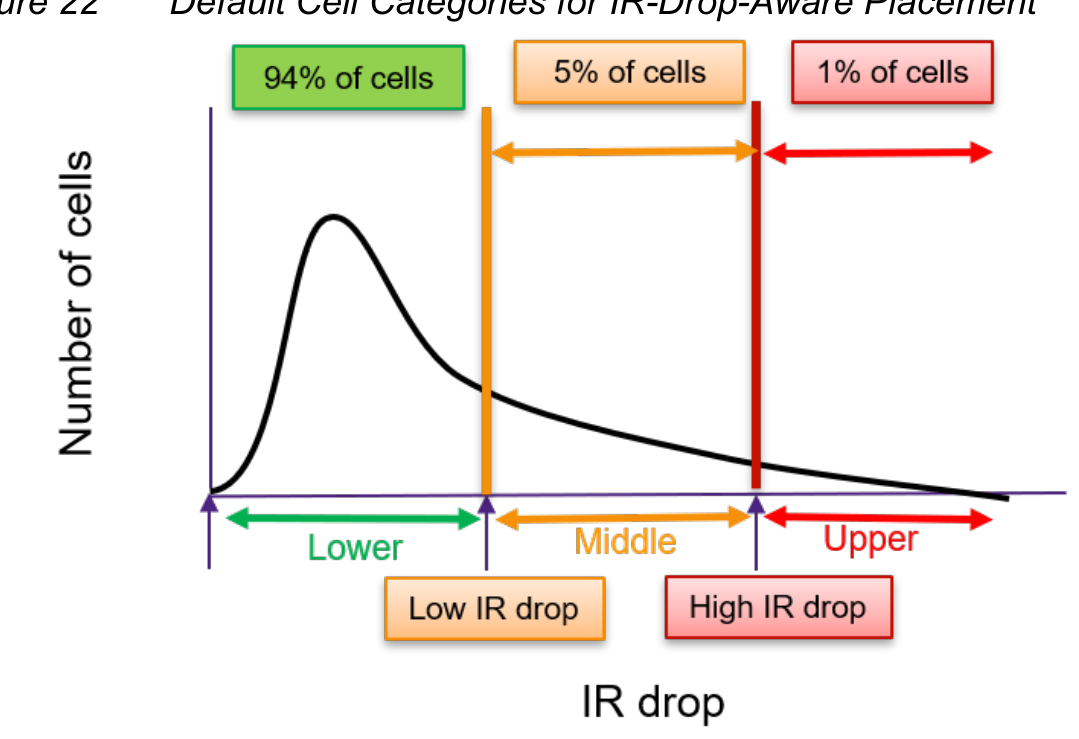
\includegraphics[width=0.92\textwidth,keepaspectratio]{figures/fig-ch2b-ir-drop-categories.png}
\caption{IR-Drop 感知布局的默认单元类别}
\label{fig:ch2b-ir-drop-categories}
\end{figure}

默认按图~\ref{fig:ch2b-ir-drop-categories} 所示准则选择三类单元：
\begin{itemize}
  \item 上层类别：压降最高的约 1\% 单元；布局时摊开力度最大。
  \item 中层类别：接下来约 5\% 单元；摊开力度小于上层。
  \item 下层类别：其余单元；工具不对其进行摊开。
\end{itemize}

可用 \appopt{place.coarse.ir\_drop\_default\_target\_high\_percentage} 与 \appopt{place.coarse.ir\_drop\_default\_target\_low\_percentage} 更改上层与中层的百分比。例如，上层取前 2\%，中层取接下来 6\%：
\begin{lstlisting}
fc_shell> set_app_options \
   -name place.coarse.ir_drop_default_target_high_percentage \
   -value 2.0
fc_shell> set_app_options \
   -name place.coarse.ir_drop_default_target_low_percentage \
   -value 6.0
\end{lstlisting}

也可不用单元总数百分比，而用压降相对电源电压的百分比定义类别：将 \appopt{place.coarse.ir\_drop\_default\_target\_high\_population} 与 \appopt{place.coarse.ir\_drop\_default\_target\_low\_population} 设为 \texttt{false}（默认为 \texttt{true}）。

例如，压降大于电源电压 8\% 的单元归入上层，4\%--8\% 归入中层：
\begin{lstlisting}
fc_shell> set_app_options \
   -name place.coarse.ir_drop_default_target_high_population \
   -value false
fc_shell> set_app_options \
   -name place.coarse.ir_drop_default_target_high_percentage \
   -value 8.0
fc_shell> set_app_options \
   -name place.coarse.ir_drop_default_target_low_population \
   -value false
fc_shell> set_app_options \
   -name place.coarse.ir_drop_default_target_low_percentage \
   -value 4.0
\end{lstlisting}

也可混合：上层用单元总数百分比，中层用压降相对电源电压百分比，或反之。例如上层取前 2\% 单元，中层取压降大于电源电压 4\% 的后续单元：
\begin{lstlisting}
fc_shell> set_app_options \
   -name place.coarse.ir_drop_default_target_high_population \
   -value true
fc_shell> set_app_options \
   -name place.coarse.ir_drop_default_target_high_percentage \
   -value 2.0
fc_shell> set_app_options \
   -name place.coarse.ir_drop_default_target_low_population \
   -value false
fc_shell> set_app_options \
   -name place.coarse.ir_drop_default_target_low_percentage \
   -value 4.0
\end{lstlisting}

可用 \cmd{set\_placement\_ir\_drop\_target} 为特定 voltage area 设置约束。例如，将 VA1 中前 1.5\% 单元归入上层、接下来 4.5\% 归入中层：
\begin{lstlisting}
fc_shell> set_placement_ir_drop_target VA1 high 1.5
fc_shell> set_placement_ir_drop_target VA1 low 4.5
\end{lstlisting}

将 VA2 中压降大于电源电压 10\% 的单元归入上层，5\%--10\% 归入中层：
\begin{lstlisting}
fc_shell> set_placement_ir_drop_target VA2 high 10 -irdrop
fc_shell> set_placement_ir_drop_target VA2 low 5 -irdrop
\end{lstlisting}

获取、报告与重置基于 voltage area 的约束，分别使用 \cmd{get\_placement\_ir\_drop\_target}、\cmd{report\_placement\_ir\_drop\_target} 与 \cmd{reset\_placement\_ir\_drop\_target}。

\subsection{布局时分散 Repeater 单元}
\subsubsection*{Spreading Repeater Cells During Placement}

若 block 在宏单元或 blockage 边缘/角落有大量 repeater 链（buffer、inverter 或流水线寄存器），工具可能沿边缘/角落聚集单元从而加剧拥塞。可在运行 \cmd{create\_placement}、\cmd{place\_opt} 或 \cmd{clock\_opt} 前将 \appopt{place.coarse.spread\_repeater\_paths} 设为 \texttt{true}；工具会沿正交方向摊开 repeater，以降低边缘与角落拥塞。

% ============================================================
\section{指定合法化设置}
\subsection*{Specifying Legalization Settings}

工具在设计流程多个阶段执行合法化。以下主题说明如何控制合法化：
\begin{itemize}
  \item 合法化期间最小化大位移
  \item 合法化期间优化 Pin Access
  \item 启用高级 PG Net 检查
  \item 启用高级合法化算法
  \item 设置 Variant 感知合法化
  \item 检查库单元是否可合法放置
\end{itemize}

\subsection{合法化期间最小化大位移}
\subsubsection*{Minimizing Large Displacements During Legalization}

要最小化合法化时单元大位移，可启用：
\begin{itemize}
  \item 朝向优化：将 \appopt{place.legalize.optimize\_orientations} 设为 \texttt{true}。\\
        工具会考虑翻转单元朝向以减小合法化位移。
  \item Stream placement：将 \appopt{place.legalize.stream\_place} 设为 \texttt{true}。\\
        工具将许多单元小幅移动，避免单颗单元大幅移动。可用 \appopt{place.legalize.stream\_effort} 与 \appopt{place.legalize.stream\_effort\_limit} 进一步控制。
\end{itemize}

\subsection{合法化期间优化 Pin Access}
\subsubsection*{Optimizing Pin Access During Legalization}

对先进工艺节点，为改善高 pin 密度区域的可布线性，可通过重分布单元启用 pin 优化：将 \appopt{place.legalize.optimize\_pin\_access\_using\_cell\_spacing} 设为 \texttt{true}。

\subsection{启用高级 PG Net 检查}
\subsubsection*{Enabling Advanced PG Net Checks}

对 12~nm、7~nm 或更小等先进节点，可将 \appopt{place.legalize.enable\_advanced\_prerouted\_net\_check} 设为 \texttt{true}，启用单元与预布线 PG net 之间的高级物理 DRC 检查。

启用后，可用 \appopt{place.legalize.advanced\_layer\_access\_check} 与 \appopt{place.legalize.advanced\_libpin\_access\_check} 进一步控制标准单元 pin 的可达性检查；对多数设计，默认行为已适用。

\subsection{启用高级合法化算法}
\subsubsection*{Enabling Advanced Legalization Algorithms}

要将用于 2D 规则检查与单元交互的高级合法化算法启用（可缩短合法化 runtime），将 \appopt{place.legalize.enable\_advanced\_legalizer} 设为 \texttt{true}。

要指定未自动检测的附加高级合法化规则，设置 \appopt{place.legalize.enable\_advanced\_legalizer\_rules}。

启用高级合法化算法后，默认在 pin access 优化时对齐垂直 pin shape 以改善可布线性。也可通过 \appopt{place.legalize.optimize\_pin\_access\_strategies} 指定附加策略，见下表。

\begin{table}[htbp]
\centering
\caption{\texttt{place.legalize.optimize\_pin\_access\_strategies} 设置（原书 Table 8）}
\label{tab:ch2b-pin-access-strategies}
\begin{tabularx}{\textwidth}{@{}X l@{}}
\toprule
\textbf{目的} & \textbf{使用的设置} \\
\midrule
对齐水平 pin shape & \texttt{horizontal\_align} \\
将单元移离高 pin 密度区域 & \texttt{avoid\_high\_pin\_density} \\
同时做以上两者 & \texttt{horizontal\_align avoid\_high\_pin\_density} \\
\bottomrule
\end{tabularx}
\end{table}

高级合法化与合法性检查期间，工具可同时检查多单元与 PG net shape 之间的 DRC。启用：将 \appopt{place.legalize.enable\_multi\_cell\_pnet\_checks} 设为 \texttt{true}。

要在最后一次 \cmd{route\_opt} 或 \cmd{route\_auto} 之后启用多单元检查，将下列应用选项设为 \texttt{true}（须先启用 \appopt{place.legalize.enable\_multi\_cell\_pnet\_checks}），有助于在考虑 QoR 的同时改善 runtime：
\begin{itemize}
  \item \appopt{place.legalize.enable\_multi\_cell\_access\_check}：考虑邻接单元与附近预布线 PG net shape 对单元 pin access 的影响。默认 \texttt{false}。
  \item \appopt{place.legalize.enable\_multi\_cell\_track\_capacity\_check}：分析该单元 pin 与邻接单元的 track 容量。Track capacity 估计该区域布线 track 是否足以访问全部指定 pin。启用本选项前须先启用 \appopt{place.legalize.enable\_multi\_cell\_access\_check}。默认 \texttt{false}。
\end{itemize}

启用多线程高级合法化：
\begin{enumerate}
  \item 将 \appopt{place.legalize.enable\_threaded\_advanced\_legalizer} 设为 \texttt{true}。
  \item 按「配置多线程」完成多线程配置。
\end{enumerate}

执行多线程高级合法性检查：
\begin{enumerate}
  \item 将 \appopt{place.legalize.enable\_advanced\_legalizer} 设为 \texttt{true}。
  \item 按「配置多线程」完成多线程配置。
  \item 用 \cmd{check\_legality} 执行合法性检查。
\end{enumerate}

\subsection{设置 Variant 感知合法化}
\subsubsection*{Setting Up for Variant-Aware Legalization}

某些库提供功能等效、但可在不同位置合法化的单元集合。工具可通过用 variant 替换单元来合法化，而不必搬移单元。

下图示出 pin 位置不同的功能等效单元。使用 variant 感知合法化时，若单元 pin 未对齐 track，工具可尝试用其 variant 使 pin 对齐 track。

\begin{figure}[htbp]
\centering
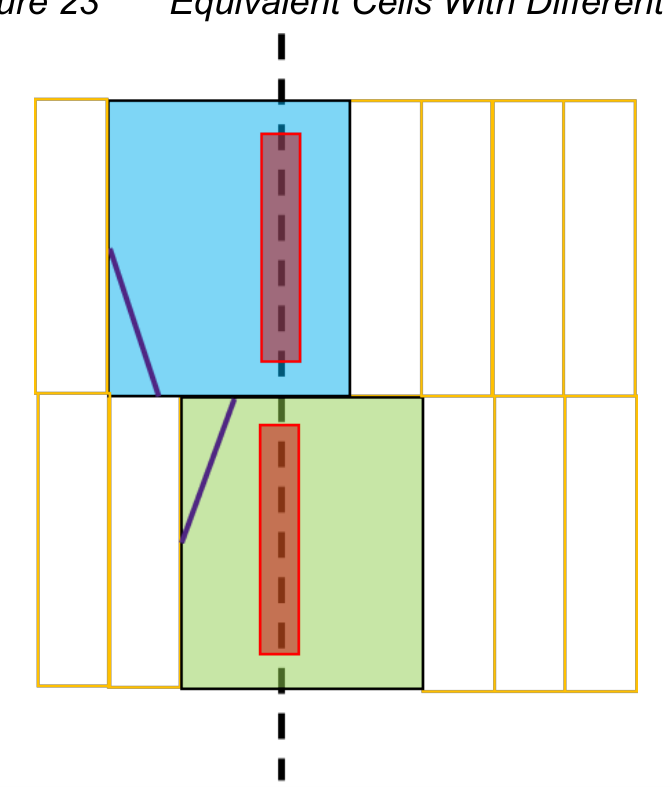
\includegraphics[width=0.45\textwidth,keepaspectratio]{figures/fig-ch2b-equiv-pin-loc.png}
\caption{Pin 位置不同的等效单元}
\label{fig:ch2b-equiv-pin-loc}
\end{figure}

下图示出 pin 颜色不同的功能等效单元，须对齐同色 track。若 pin 未对齐对应颜色 track，工具可尝试使用不同颜色 pin 的 variant 并对齐到合适颜色的 track。

\begin{figure}[htbp]
\centering
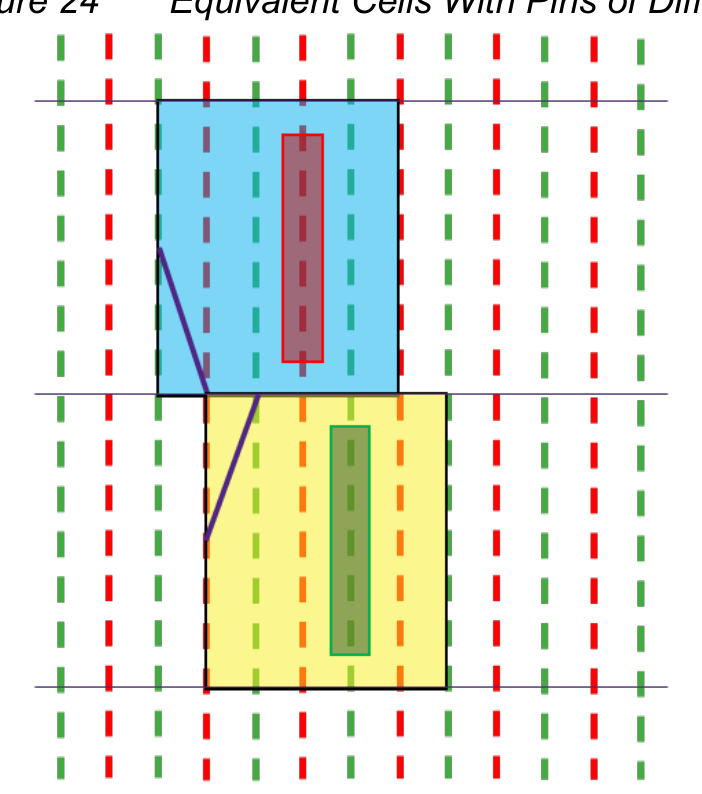
\includegraphics[width=0.45\textwidth,keepaspectratio]{figures/fig-ch2b-equiv-pin-color.png}
\caption{Pin 颜色不同的等效单元}
\label{fig:ch2b-equiv-pin-color}
\end{figure}

设置参考库与设计以支持 variant 感知合法化，需完成：
\begin{itemize}
  \item 定义等效单元组
  \item 启用 Variant 感知合法化
\end{itemize}

\subsubsection{定义等效单元组}
\subsubsection*{Defining Equivalent Cell Groups}

Library Compiler 支持从 Liberty 源文件创建 variant-ready 库。Liberty 中的 \texttt{physical\_variant\_cells} 属性定义单元的 variant；若该属性存在，编译后的库即为 variant ready。

若逻辑库非 variant ready，可在 Library Manager 的库准备阶段用 \cmd{create\_cell\_groups} 定义等效单元组。例如向已有参考库添加等效单元组：
\begin{lstlisting}
lm_shell> create_workspace -flow edit LIB.ndm
lm_shell> create_cell_group -name A [get_lib_cells MY_LIB/A_*]
lm_shell> create_cell_group -name B [get_lib_cells MY_LIB/B_*]
lm_shell> check_workspace
lm_shell> commit_workspace
\end{lstlisting}

在 Library Manager 或 Fusion Compiler 中，可用 \cmd{report\_cell\_groups} 报告库中的等效单元组；该命令既报告 variant-ready 逻辑库 Liberty 中定义的组，也报告 Library Manager 中用 \cmd{create\_cell\_groups} 定义的组。

\subsubsection{启用 Variant 感知合法化}
\subsubsection*{Enabling Variant-Aware Legalization}

将 \appopt{place.legalize.enable\_variant\_aware} 设为 \texttt{true} 以启用。启用后，工具优先用 variant 交换违例单元来修复合法化 DRC，而非搬移；若无 variant，再移到合法位置。

Variant 感知合法化中的 pin-track 与 pin-color 对齐，须将下列应用选项设为 \texttt{true}：
\begin{itemize}
  \item \appopt{place.legalize.enable\_prerouted\_net\_check}
  \item \appopt{place.legalize.enable\_pin\_color\_alignment\_check}
\end{itemize}
并用 \appopt{place.legalize.pin\_color\_alignment\_layers} 指定要对齐的层。

\subsection{检查库单元是否可合法放置}
\subsubsection*{Checking if Library Cells Are Legally Placeable}

指定全部布局与合法化约束及设置后，可用 \cmd{analyze\_lib\_cell\_placement -lib\_cells} 检查特定库单元能否在 block 中合法放置。
\begin{itemize}
  \item 用 \opt{-region} 将分析限制在 core 的特定区域（默认搜索整个 core）。
  \item 用 \opt{-trials} 限制分析的 site 数量（默认随机分析 1000 个 site）。设为 0 则分析全部空闲 site，可能增加 runtime。
  \item 用 \opt{-no\_pdc} 或 \opt{-no\_adv} 在分析时忽略物理设计约束或高级设计规则。
  \item 用 \opt{-threshold} 仅报告未达指定阈值的相对布局组：仅当单元可放置 site 占所分析 site 的百分比低于阈值时才报告。
  \item 用 \opt{-max\_cells} 限制报告单元数（默认 100，从通过率最差的库单元开始）。
\end{itemize}

若 block 中某些库单元通过率极低，合法化时会导致大位移与更长 runtime。此时应检查电源计划、单元版图与合法化设置以提高通过率。

下列示例分析当前 block 中有实例的全部库单元：
\begin{lstlisting}
fc_shell> analyze_lib_cell_placement -lib_cells [add_to_collection \
 -unique "" [get_attribute [get_cells -physical_context] ref_phys_block]]

Analyzing 215 lib cell(s).
Warning: Routing direction of metal layer PO is neither "horizontal" nor
 "vertical". PDC checks will not be performed on this layer. (PDC-003)

PDC app_options settings =========
        place.legalize.enable_prerouted_net_check: 1
        place.legalize.num_tracks_for_access_check: 1
        place.legalize.use_eol_spacing_for_access_check: 0
        place.legalize.allow_touch_track_for_access_check: 1
        place.legalize.reduce_conservatism_in_eol_check: 0
        place.legalize.preroute_shape_merge_distance: 0.0

Layer M1: cached 0 shapes out of 869 total shapes.
Layer M2: cached 773 shapes out of 773 total shapes.
Cached 41757 vias out of 99466 total vias.
0.0%...2.0%...4.0%...6.0%...8.0%...10.0%........

  Lib Cell                                        Pass Rate
  ----------------------------------              ---------
  saed32_lvt_lsup:LSUPX1_LVT.frame                0.4450
  saed32_lvt_lsup:LSUPX8_LVT.frame                0.4780
  saed32_lvt_lsup:LSUPX2_LVT.frame                0.4810
  saed32_lvt_lsup:LSUPX4_LVT.frame                0.5040
  ..............
  saed32_rvt_std:HADDX1_RVT.frame                 0.8600
  saed32_lvt_std:OA21X1_LVT.frame                 0.8610
\end{lstlisting}

% ============================================================
\section{控制单元、Net、Pin 与 Port 的优化}
\subsection*{Controlling the Optimization of Cells, Nets, Pins, and Ports}

以下主题说明如何控制单元、net、pin 与 port 的优化：
\begin{itemize}
  \item 优化期间保留单元与 Net
  \item 将优化限制为仅做单元尺寸调整
  \item 优化期间保留网络
  \item 标记时钟网络
  \item 禁用设计规则检查（DRC）
  \item 尺寸调整期间保留 Pin 名称
  \item 保留已有层次的 Port
  \item 隔离输入与输出 Port
  \item 修复多 Port Net
  \item 控制向 Module、层次单元与 Voltage Area 添加新单元
  \item 为优化指定单元名前缀
\end{itemize}

\subsection{优化期间保留单元与 Net}
\subsubsection*{Preserving Cells and Nets During Optimization}

要用 \cmd{set\_dont\_touch} 在优化期间保留设计对象。该命令对当前设计中的单元、net、reference 与子设计设置 \texttt{dont\_touch} 属性，防止优化时修改或替换。

下表说明工具如何在优化期间保留各类设计对象。

\begin{table}[htbp]
\centering
\caption{优化期间 \texttt{dont\_touch} 对各设计对象的行为}
\begin{tabularx}{\textwidth}{@{}l X@{}}
\toprule
\textbf{设计对象} & \textbf{工具行为} \\
\midrule
单元 & 将单元排除在优化之外。 \\
Net & 保留各 pin 到该 net 的连接。 \\
Module、设计、库单元 & 阻止优化所有引用它们的实例。 \\
层次单元或 module & 将该单元及其全部子单元排除在优化之外。 \\
\bottomrule
\end{tabularx}
\end{table}

使用 \cmd{set\_dont\_touch} 时请注意：
\begin{itemize}
  \item 该命令阻止层次 ungrouping。
  \item 子单元必须继承其父 module 的同一 \texttt{dont\_touch} 属性。例如，父 module 已标 \texttt{dont\_touch} 时，不能单独移除子单元上的该属性。
  \item 仅对完全映射（fully mapped）的逻辑使用，包括单元、module、设计，以及周围逻辑已完全映射的 net。
  \item \texttt{dont\_touch} 优先级高于 \texttt{boundary\_optimization} 与 \texttt{size\_only}。
\end{itemize}

报告带 \texttt{dont\_touch} 的设计对象，使用 \cmd{report\_dont\_touch}。

下列命令在单元 A 上设置 \texttt{dont\_touch}：
\begin{lstlisting}
fc_shell> set_dont_touch [get_cells A] true
\end{lstlisting}

移除该属性可用 \cmd{remove\_attributes}，或将 \cmd{set\_dont\_touch} 设为 \texttt{false}：
\begin{lstlisting}
fc_shell> remove_attributes [get_cells A] dont_touch
fc_shell> set_dont_touch [get_cells A] false
\end{lstlisting}

下表汇总可对 module、单元、net 与库单元设置、移除或报告 \texttt{dont\_touch} 的命令支持情况。Yes 表示支持，No 表示不支持。

\begin{table}[htbp]
\centering
\caption{\texttt{dont\_touch} 属性的命令支持（原书 Table 9）}
\label{tab:ch2b-dont-touch}
\begin{tabularx}{\textwidth}{@{}l c c c c@{}}
\toprule
\textbf{命令} & \textbf{Module} & \textbf{单元（实例）} & \textbf{Net} & \textbf{库单元} \\
\midrule
\cmd{set\_dont\_touch} & Yes & Yes & Yes & Yes \\
\cmd{set\_attribute} & Yes & Yes & Yes & Yes \\
\cmd{define\_user\_attribute} & No & No & No & No \\
\cmd{get\_attribute} & Yes & Yes & Yes & Yes \\
\cmd{remove\_attributes} & Yes & Yes & Yes & Yes \\
\cmd{report\_dont\_touch} & Yes & Yes & Yes & No \\
\cmd{set\_dont\_touch\_unmapped\_object} & No & No & Yes & NA \\
\bottomrule
\end{tabularx}
\end{table}

\subsection{将优化限制为仅做单元尺寸调整}
\subsubsection*{Restricting Optimization to Cell Sizing Only}

要允许优化期间仅对单元或实例做尺寸调整，使用 \cmd{set\_size\_only}。该命令对指定单元或实例设置 \texttt{size\_only} 属性，防止除 sizing 外的修改或替换。

查询该属性可用 \cmd{report\_attributes}、\cmd{get\_attribute} 或 \cmd{report\_cells}；移除可用 \cmd{remove\_attributes}，或将 \cmd{set\_size\_only} 设为 \texttt{false}。

在特定单元上设置：
\begin{lstlisting}
fc_shell> set_size_only [get_cells cell_name] true
\end{lstlisting}

查询：
\begin{lstlisting}
fc_shell> get_attribute [get_cells cell_name] size_only
\end{lstlisting}

报告当前设计全部 \texttt{size\_only} 信息：
\begin{lstlisting}
fc_shell> report_size_only -all
\end{lstlisting}

\subsection{优化期间保留网络}
\subsubsection*{Preserving Networks During Optimization}

可用 \cmd{set\_dont\_touch\_network} 在优化期间保留时钟树等网络。该命令对时钟、pin 或 port 设置 \texttt{dont\_touch}，防止网络传递扇出中的单元与 net 被修改或替换。

默认同时保留时钟路径与 clock-as-data 路径，并在网络层次中传播 \texttt{dont\_touch}。仅保留时钟路径时指定 \opt{-clock\_only}；从网络移除该属性时指定 \opt{-clear}。

在 CLK 时钟网络上设置：
\begin{lstlisting}
fc_shell> set_dont_touch_network [get_clocks CLK]
\end{lstlisting}

仅对 CLK 时钟路径：
\begin{lstlisting}
fc_shell> set_dont_touch_network [get_clocks CLK] -clock_only
\end{lstlisting}

移除：
\begin{lstlisting}
fc_shell> set_dont_touch_network [get_clocks CLK] -clear
\end{lstlisting}

\subsection{标记时钟网络}
\subsubsection*{Marking the Clock Networks}

若 block 尚无时钟树，应使用 ideal clock 进行优化。将全部时钟网络标为 ideal：
\begin{lstlisting}
foreach_in_collection mode [all_modes] {
  current_mode $mode
  set_ideal_network [all_fanout -flat -clock_tree]
}
\end{lstlisting}

为建模时钟树对布局的影响，还应为每个时钟用 \cmd{set\_clock\_uncertainty}、\cmd{set\_clock\_latency} 与 \cmd{set\_clock\_transition} 定义 uncertainty、latency 与 transition 约束。

在执行时钟树综合前，必须用 \cmd{remove\_ideal\_network} 移除时钟树扇出上的 ideal 设置。

\subsection{禁用设计规则检查（DRC）}
\subsubsection*{Disabling Design Rule Checking (DRC)}

可用 \cmd{set\_auto\_disable\_drc\_nets} 禁用时钟、常数、scan enable 与 scan clock net 上的设计规则检查。

用该命令的选项控制当前设计中特定 net 的 DRC，见表~\ref{tab:ch2b-auto-disable-drc}。

\begin{table}[htbp]
\centering
\caption{\texttt{set\_auto\_disable\_drc\_nets} 的选项（原书 Table 10）}
\label{tab:ch2b-auto-disable-drc}
\begin{tabularx}{\textwidth}{@{}l X@{}}
\toprule
\textbf{选项} & \textbf{作用} \\
\midrule
\opt{-none} & 对全部 net 启用 DRC。 \\
\opt{-all} & 对全部时钟、常数、scan enable 与 scan clock net 禁用 DRC。 \\
\opt{-constant true | false} & 对常数 net 禁用（\texttt{true}）或启用（\texttt{false}）DRC。 \\
\opt{-on\_clock\_network true | false} & 对时钟网络禁用或启用 DRC。 \\
\opt{-scan true | false} & 对 scan enable 与 scan clock net 禁用或启用 DRC。 \\
\bottomrule
\end{tabularx}
\end{table}

例如，对全部此类 net 启用 DRC：
\begin{lstlisting}
fc_shell> set_auto_disable_drc_nets -none
\end{lstlisting}

对连接时钟与常数的 net 禁用 DRC：
\begin{lstlisting}
fc_shell> set_auto_disable_drc_nets \
   -on_clock_network true -constant true
\end{lstlisting}

\begin{figure}[htbp]
\centering
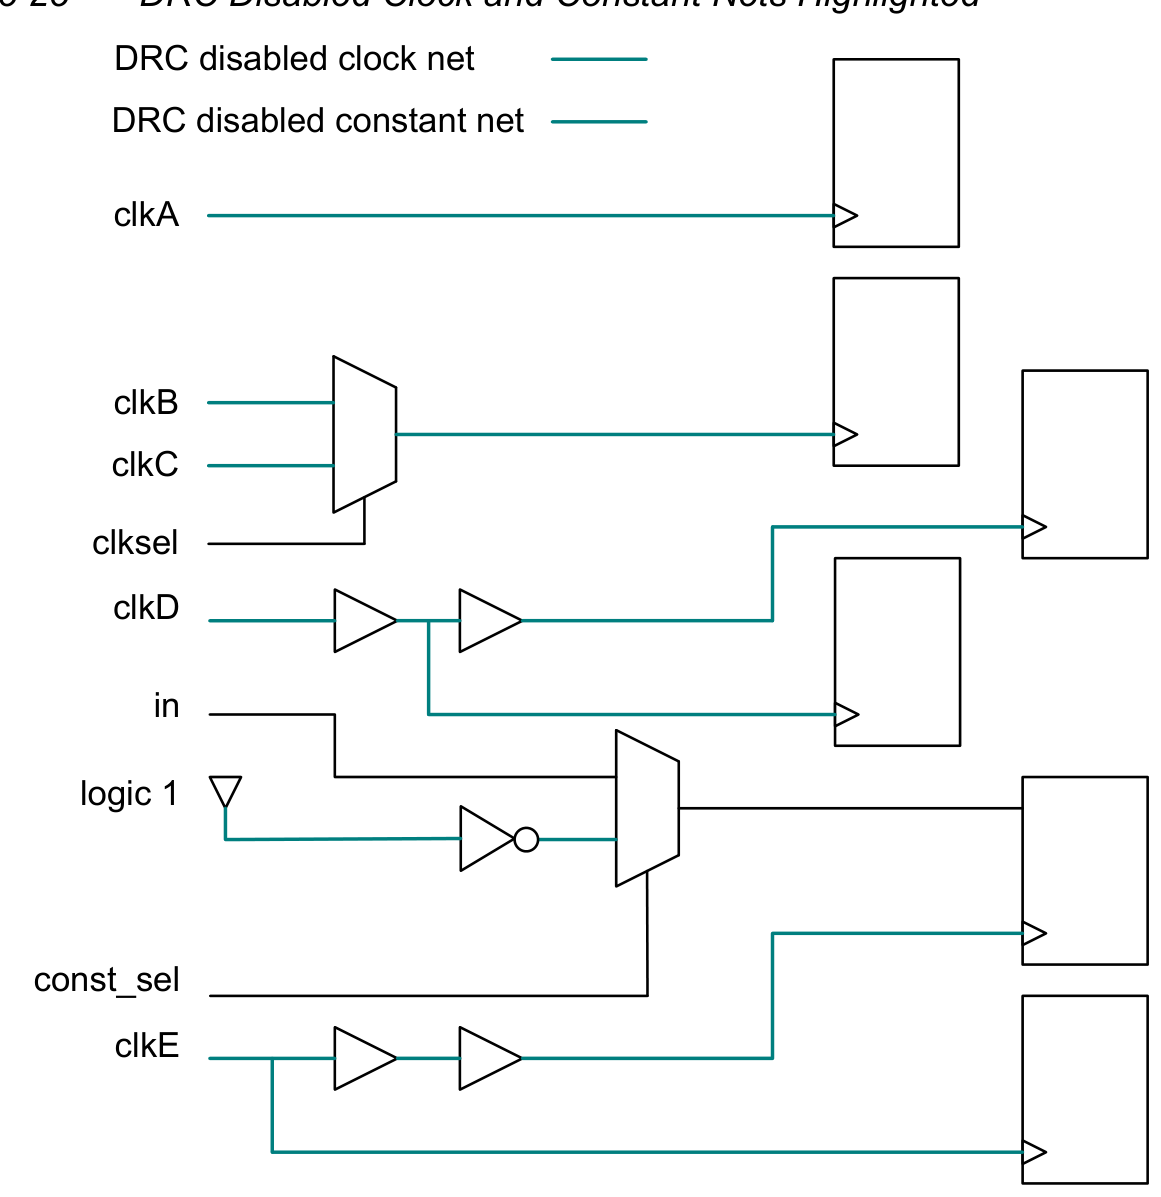
\includegraphics[width=0.85\textwidth,keepaspectratio]{figures/fig-ch2b-drc-disabled.png}
\caption{已禁用 DRC 的时钟与常数 Net}
\label{fig:ch2b-drc-disabled}
\end{figure}

\subsection{尺寸调整期间保留 Pin 名称}
\subsubsection*{Preserving Pin Names During Sizing}

默认情况下，若结果电路功能等价，优化可在 sizing 时更改叶子单元的 pin 名称。Fusion Compiler 会自动更新内部约束版本以反映异常约束中涉及的新 pin 名。若发生此情况，用于约束 block 的原始约束不能再用于 signoff；必须从 Fusion Compiler 写出约束并随结果 block 一并使用。

该行为为优化引擎选择单元与改善代价函数提供最大灵活性。可通过设置 \appopt{opt.common.preserve\_pin\_names} 限制 sizing，使约束在优化中保持不变。默认值为 \texttt{never}，可取 \texttt{never} 或 \texttt{always}。

限制为仅 pin 名等价的单元：
\begin{lstlisting}
fc_shell> set_app_options \
   -name opt.common.preserve_pin_names -value always
\end{lstlisting}

恢复默认：
\begin{lstlisting}
fc_shell> set_app_options \
   -name opt.common.preserve_pin_names -value never
\end{lstlisting}

\subsection{保留已有层次的 Port}
\subsubsection*{Preserving Ports of Existing Hierarchies}

优化与时钟树综合期间，工具可在已有层次 block 上创建新 port。要阻止此行为，使用 \cmd{set\_freeze\_ports}，并将对应单元实例的 \texttt{freeze\_clock\_port} 属性设为 \texttt{true}。

可用 \opt{-clock}、\opt{-data} 或 \opt{-all} 分别阻止添加时钟 port、数据 port 或两者。例如，阻止在 \texttt{MBX22} 上创建额外时钟 port：
\begin{lstlisting}
fc_shell> set_freeze_ports -clock [get_cells MBX22] true
\end{lstlisting}

报告 freeze-port 设置使用 \cmd{report\_freeze\_ports}。

\subsection{隔离输入与输出 Port}
\subsubsection*{Isolating Input and Output Ports}

可隔离输入与输出 port 以提高时序模型精度。在指定输入或输出 port 插入隔离逻辑，使用 \cmd{set\_isolate\_ports}。隔离逻辑可以是 buffer 或一对 inverter；默认放置 buffer 以隔离：
\begin{itemize}
  \item 输入 port 与其扇出网络
  \item 输出 port 与其驱动
\end{itemize}

使用 \opt{-force} 时，工具确保 \opt{-driver} 指定的库单元不会被 sizing。

工具不会在下列 port 上放置隔离逻辑：
\begin{itemize}
  \item 双向 port
  \item 定义为时钟源或电源 pin 的 port
  \item 连接到带 \texttt{dont\_touch} 属性的 net 的 port
\end{itemize}

\subsubsection{示例}
\subsubsection*{Example}

下列命令插入隔离逻辑：
\begin{itemize}
  \item 输入 port \texttt{in3}：buffer
  \item 输出 port \texttt{out1}：buffer
  \item 输出 port \texttt{out3}：\texttt{LIBCELL\_BUFF} 库单元
  \item 输出 port \texttt{out4}：一对 inverter
\end{itemize}
\begin{lstlisting}
fc_shell> set_isolate_ports {in3 out1}
fc_shell> set_isolate_ports -driver LIBCELL_BUFF out3 -force
fc_shell> set_isolate_ports -type inverter out4
\end{lstlisting}

\begin{figure}[htbp]
\centering
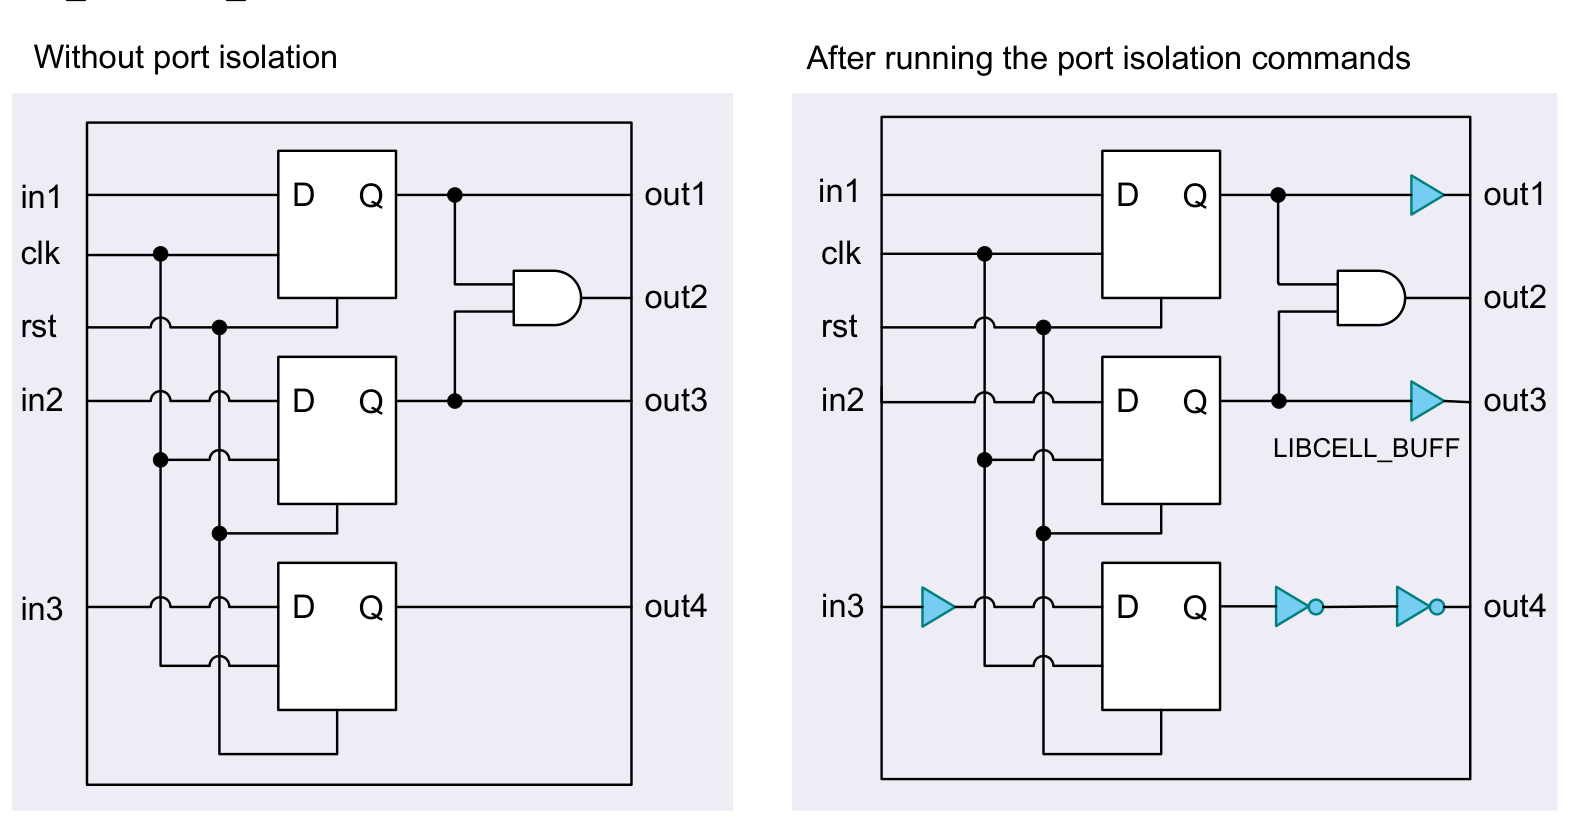
\includegraphics[width=0.95\textwidth,keepaspectratio]{figures/fig-ch2b-port-isolation.png}
\caption{Port 隔离逻辑插入前后对比}
\label{fig:ch2b-port-isolation}
\end{figure}

\subsection{修复多 Port Net}
\subsubsection*{Fixing Multiple-Port Nets}

多 port net 包括：
\begin{itemize}
  \item Feedthrough net：输入 port 直接馈入输出 port
  \item 连接到多个输出 port 的 net（逻辑等价输出）
\end{itemize}

\begin{figure}[htbp]
\centering
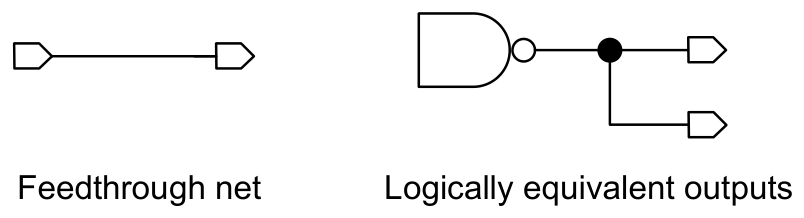
\includegraphics[width=0.75\textwidth,keepaspectratio]{figures/fig-ch2b-multiport-nets.png}
\caption{多 Port Net 类型示意}
\label{fig:ch2b-multiport-nets}
\end{figure}

门级网表中以 \texttt{assign} 语句表示的多 port net，可能在后续流程导致设计规则违例。默认优化期间工具不修复多 port net。

要将 \appopt{opt.port.eliminate\_verilog\_assign} 设为 \texttt{true} 以修复（默认 \texttt{false}）。修复时工具依次：
\begin{enumerate}
  \item 尽可能重连，使每条 net 只连到一个层次 port。\\
        工具优先重连以避免不必要的 buffering；因默认启用 boundary optimization，也会跨层次重连。
  \item 对未能通过重连修复的 net 插入 buffer 或 inverter。
\end{enumerate}

\subsection{控制向 Module、层次单元与 Voltage Area 添加新单元}
\subsubsection*{Controlling the Addition of New Cells to Modules, Hierarchical Cells, and Voltage Areas}

控制向下列对象添加新单元：
\begin{itemize}
  \item Module 或层次单元：使用 \cmd{set\_allow\_new\_cells}
  \item Voltage area：在 \cmd{create\_voltage\_area\_rule} 中使用 \opt{-allow\_new\_cells}
\end{itemize}

可用这些设置阻止向 abut 设计的顶层层次与 voltage area 添加新单元。设置保存在设计库中，并在整个实现流程中被工具遵守。

阻止向顶层 module 添加：
\begin{lstlisting}
fc_shell> set_allow_new_cells \
   [get_attribute [current_block] top_module] false
\end{lstlisting}

阻止向 \texttt{M1} module 添加：
\begin{lstlisting}
fc_shell> set_allow_new_cells [get_modules M1] false
\end{lstlisting}

阻止向 \texttt{U22} 层次单元添加：
\begin{lstlisting}
fc_shell> set_allow_new_cells [get_cells U22] false
\end{lstlisting}

阻止向 \texttt{VA1} voltage area 添加：
\begin{lstlisting}
fc_shell> create_voltage_area_rule -name VA1_rule \
   -allow_new_cells false -voltage_areas VA1
\end{lstlisting}

\subsection{为优化指定单元名前缀}
\subsubsection*{Specifying a Cell Name Prefix for Optimization}

可用 \appopt{opt.common.user\_instance\_name\_prefix} 为优化期间在数据 net 上添加的单元指定名前缀。

下列示例为数据 net 上添加的单元指定名前缀：
\begin{itemize}
  \item \cmd{place\_opt} 期间：\texttt{PO\_}
  \item \cmd{clock\_opt} 期间：\texttt{CO\_}
  \item \cmd{route\_opt} 期间：\texttt{RO\_}
\end{itemize}
\begin{lstlisting}
fc_shell> set_app_options \
   -name opt.common.user_instance_name_prefix -value "PO_"
fc_shell> place_opt
fc_shell> set_app_options \
   -name opt.common.user_instance_name_prefix -value "CO_"
fc_shell> clock_opt
fc_shell> set_app_options \
   -name opt.common.user_instance_name_prefix -value "PO_"
fc_shell> route_opt
\end{lstlisting}

为时钟树综合期间在时钟网络上添加的单元指定名前缀，使用 \appopt{cts.common.user\_instance\_name\_prefix}，见「为时钟单元定义名前缀」。

% ============================================================
\section{指定布线前优化设置}
\subsection*{Specifying Settings for Preroute Optimization}

为性能、功耗与面积（PPA）优化设计是工具的主要目标之一。以下主题说明如何在布线前阶段指定性能、功耗与面积优化设置：
\begin{itemize}
  \item 控制 \cmd{place\_opt} 的 DFT 优化
  \item 指定布线前优化的寄生参数估计设置
  \item 指定布线前优化的自动 Via Ladder 插入设置
  \item 在高利用率区域启用面积回收
  \item 启用高级逻辑重构
\end{itemize}

\subsection{控制 \texttt{place\_opt} 的 DFT 优化}
\subsubsection*{Controlling DFT Optimization for the place\_opt Command}

若 block 含 scan chain，默认 \cmd{create\_placement}、\cmd{place\_opt} 与 \cmd{clock\_opt} 会执行物理 DFT 优化。初始布局时，工具忽略 scan chain，专注功能 net 的 QoR；初始布局后，基于初始布局对 scan chain 重新分区（repartition）并重排序（reorder），以进一步改善 QoR。

利用物理信息对 scan chain 重分区与重排序可：
\begin{itemize}
  \item 缩短 scan chain 线长
  \item 最小化拥塞并改善可布线性
\end{itemize}

对含 scan chain 的 block 运行上述命令时，block 必须包含 SCANDEF 信息。用 \cmd{read\_def} 标注 SCANDEF：
\begin{lstlisting}
fc_shell> read_def ./myscan.def
\end{lstlisting}

\begin{noteBox}
若此前已在 block 上标注 scan chain 信息，且 SCANDEF 中某 chain 与已有 scan chain 同名，则保留已有 chain 定义。
\end{noteBox}

SCANDEF 文件指定 scan 路径所用的 scan chain 组件及其 pin，以及重排序约束。为获最佳效果，应使用 TestMAX DFT 做 DFT 插入，并用 Design Compiler topographical mode 生成 SCANDEF。DFT 插入见 \textit{TestMAX DFT User Guide}；生成 SCANDEF 见 \textit{Design Compiler User Guide}。

工具在 DFT 优化中使用 SCANDEF 信息。可按下表控制 DFT 优化。

\begin{table}[htbp]
\centering
\caption{控制 DFT 优化的设置（原书 Table 11）}
\label{tab:ch2b-dft-opt}
\begin{tabularx}{\textwidth}{@{}X X@{}}
\toprule
\textbf{目的} & \textbf{使用的设置} \\
\midrule
对无 SCANDEF 信息的 block 运行 \cmd{create\_placement}、\cmd{place\_opt} 或 \cmd{clock\_opt} &
将 \appopt{place.coarse.continue\_on\_missing\_scandef} 设为 \texttt{true} \\
禁用 DFT 优化 &
将 \appopt{opt.dft.optimize\_scan\_chain} 设为 \texttt{false} \\
禁用 scan chain 重分区 &
将 \appopt{opt.dft.do\_repartition} 设为 \texttt{false} \\
禁用基于时序的 scan chain 重排序 &
将 \appopt{opt.dft.timing\_friendly\_reorder} 设为 \texttt{false} \\
重排序时考虑 scan 路径上的 hold 违例（CTS 后使用，以减少 scan 路径 hold 违例） &
将 \appopt{opt.dft.clock\_aware\_scan\_reorder} 设为 \texttt{true} \\
重分区与重排序时考虑 scan 路径上的 hold 违例（CTS 后使用） &
将 \appopt{opt.dft.clock\_aware\_scan\_repartition\_reorder} 设为 \texttt{false} \\
DFT 优化期间保留层次 port（启用后不做 timing-friendly 或 clock-aware DFT 优化） &
将 \appopt{opt.dft.hier\_preservation} 设为 \texttt{true} \\
\bottomrule
\end{tabularx}
\end{table}

报告 DFT 优化相关应用选项设置，使用 \cmd{report\_app\_options}。

对已布局 block 执行独立 DFT 优化，使用 \cmd{optimize\_dft}。

\subsection{指定布线前优化的寄生参数估计设置}
\subsubsection*{Specifying Parasitic Estimation Settings for the Preroute Optimization}

以下主题说明如何在布线前阶段控制寄生参数估计：
\begin{itemize}
  \item 启用基于全局布线层（GRLB）的布线前优化
  \item 为布线前优化启用 Route-Driven Estimation（RDE）
\end{itemize}

\subsubsection{启用基于全局布线层（GRLB）的布线前优化}
\subsubsection*{Enabling Global-Route-Layer-Based (GRLB) Preroute Optimization}

为改善与布线后阶段的相关性，可在 \cmd{place\_opt} 与 \cmd{clock\_opt} 期间启用基于全局布线层的 RC 估计。启用后，工具对全部 net 使用全局布线，识别每单位电阻最合适的层，并将 net 约束到最小/最大层以进行布线前 RC 估计。

用 \appopt{opt.common.use\_route\_aware\_estimation} 启用：
\begin{itemize}
  \item \texttt{auto}：仅当不同布线层的每单位电阻存在差异时启用
  \item \texttt{true}：无论层间每单位电阻是否差异均启用
\end{itemize}

若启用该功能，在执行布线前须用 \cmd{remove\_route\_aware\_estimation} 移除全部基于全局布线的估计。

\subsubsection{为布线前优化启用 Route-Driven Estimation（RDE）}
\subsubsection*{Enabling Route-Driven Estimation (RDE) for Preroute Optimization}

为改善与布线后相关性，工具可执行全局布线、基于全局布线做提取，并在优化中使用这些寄生信息。

若检测到设计所用工艺为小于 16~nm 的先进节点，默认启用该功能。对任意工艺启用：将 \appopt{opt.common.enable\_rde} 设为 \texttt{true}。

启用后，工具在 \cmd{place\_opt} 与 \cmd{clock\_opt} 的 \texttt{final\_opt} 阶段执行 route-driven 寄生估计。寄生信息存入设计库，供后续优化步骤使用。启用后，应在设计流程后续全部布线前优化步骤中保持启用。

Route-driven estimation 期间，工具遵守 \cmd{set\_extraction\_options} 的 \opt{-early\_cap\_scale}、\opt{-late\_cap\_scale}、\opt{-early\_res\_scale}、\opt{-late\_res\_scale} 所指定的电容/电阻缩放因子。

启用 RDE 时，工具忽略用于启用 GRLB RC 估计的 \appopt{opt.common.use\_route\_aware\_estimation} 设置。

\subsection{指定布线前优化的自动 Via Ladder 插入设置}
\subsubsection*{Specifying Automatic Via Ladder Insertion Settings for Preroute Optimization}

Via ladder 是从 pin 层向上延伸到上层布线层的堆叠 via。优化期间使用 via ladder 可改善设计的性能与电迁移鲁棒性。工具可在 \cmd{place\_opt} 与 \cmd{clock\_opt} 期间为时序关键路径上的单元 pin 自动插入 via ladder。

布线前优化中执行 via ladder 插入：
\begin{enumerate}
  \item 确保已按「定义 Via Ladder 规则」定义 via ladder 规则。
  \item 用 \cmd{set\_via\_ladder\_candidate} 为特定库 pin 指定可用 via ladder，见「为库 Pin 指定 Via Ladder 候选」。
  \item （可选）将 \appopt{opt.common.enable\_via\_ladder\_insertion} 设为 \texttt{true}，为关键路径启用高性能与电迁移 via ladder 插入。
  \item （可选）将 \appopt{route.global.insert\_gr\_via\_ladders} 设为 \texttt{true}，在带 via ladder 约束的 pin 上启用基于全局布线的 via ladder 插入。
  \item 用 \cmd{place\_opt} 或 \cmd{clock\_opt} 执行优化。
\end{enumerate}

\subsubsection{为库 Pin 指定 Via Ladder 候选}
\subsubsection*{Specifying Via Ladder Candidates for Library Pins}

用 \cmd{set\_via\_ladder\_candidate} 指定布线前优化中某库 pin 可用的有效 via ladder。每次命令只能指定一个 via ladder；要为同一库 pin 指定多个候选，多次调用，例如：
\begin{lstlisting}
fc_shell> set_via_ladder_candidate [get_lib_pins lib1/AND2/A1] \
   -ladder_name "VP4"
fc_shell> set_via_ladder_candidate [get_lib_pins lib1/AND2/A1] \
   -ladder_name "VP2"
\end{lstlisting}

同一库 pin 上多个 via ladder 的指定顺序表示插入优先级；应从最高优先级开始指定。上例中 \texttt{VP4} 优先于 \texttt{VP2}。

\begin{noteBox}
若同一 pin 同时适用 \texttt{pattern\_must\_join} 属性与 via ladder 候选，且两种方法估计延时相同时，via ladder 优先于基于 pattern 的 must-join 连接。
\end{noteBox}

要指定某库 pin 需要电迁移 via ladder，将 pin 属性 \texttt{is\_em\_via\_ladder\_required} 设为 \texttt{true}：
\begin{lstlisting}
fc_shell> set_attribute [get_lib_pins lib1/INV4/A] \
   is_em_via_ladder_required true
\end{lstlisting}

若将该属性设为 \texttt{true}，必须用 \cmd{set\_via\_ladder\_candidate} 将某个电迁移 via ladder 指定为候选。

可通过下列方式之一将 via ladder 标识为电迁移 via ladder：
\begin{itemize}
  \item 在工艺文件中定义 via 规则时使用 \texttt{forElectromigration=1}，例如：
\begin{lstlisting}
ViaRule "EMVP1" {
   ...
   forElectromigration=1
}
\end{lstlisting}
  \item 将 \texttt{for\_electro\_migration} 属性设为 \texttt{true}：
\begin{lstlisting}
fc_shell> set_attribute [get_via_rules EMVP1] \
   for_electro_migration true
\end{lstlisting}
\end{itemize}

\begin{seeAlsoBox}
定义 Via Ladder 规则。
\end{seeAlsoBox}

\subsection{在高利用率区域启用面积回收}
\subsubsection*{Enabling Area Recovery in Regions of High Utilization}

对因高利用率区域而无法合法化的设计，可将 \appopt{opt.common.small\_region\_area\_recovery} 设为 \texttt{true}，让工具在高利用率区域执行面积回收。

启用后，工具在 \cmd{place\_opt} 与 \cmd{clock\_opt} 期间执行面积回收，但可能轻微劣化时序 QoR。

\subsection{启用高级逻辑重构}
\subsubsection*{Enabling Advanced Logic Restructuring}

为改善面积、时序与功耗 QoR，可启用高级逻辑重构。对 \cmd{place\_opt} 与 \cmd{clock\_opt} 的 \texttt{final\_opto} 阶段，用 \appopt{opt.common.advanced\_logic\_restructuring\_mode} 启用，见下表。

\begin{table}[htbp]
\centering
\caption{\texttt{opt.common.advanced\_logic\_restructuring\_mode} 设置（原书 Table 12）}
\label{tab:ch2b-adv-restruct}
\begin{tabularx}{\textwidth}{@{}X l@{}}
\toprule
\textbf{目的} & \textbf{使用的设置} \\
\midrule
不执行重构 & \texttt{none}（默认） \\
改善面积 QoR & \texttt{area} \\
改善时序 QoR & \texttt{timing} \\
改善功耗 QoR & \texttt{power} \\
改善面积与时序 QoR & \texttt{area\_timing} \\
改善时序与功耗 QoR & \texttt{timing\_power} \\
改善面积与功耗 QoR & \texttt{area\_power} \\
改善面积、时序与功耗 QoR & \texttt{area\_timing\_power} \\
\bottomrule
\end{tabularx}
\end{table}

重构时，工具不会：
\begin{itemize}
  \item 跨逻辑层次重构
  \item 考虑带 \texttt{dont\_touch}、\texttt{size\_only} 或 \texttt{fixed} 属性的单元
  \item 在线长增加时接受结果\\
        但若设计无拥塞或布线问题，可将 \appopt{opt.common.advanced\_logic\_restructuring\_wirelength\_costing} 设为 \texttt{medium} 或 \texttt{none}（默认 \texttt{high}），使工具在线长增加时仍接受重构结果。
\end{itemize}

\begin{noteBox}
该功能需要 Digital-AF license key。
\end{noteBox}

% ============================================================
\section{设置功耗相关功能}
\subsection*{Setting Up for Power-Related Features}

以下主题说明为功耗相关功能设置设计所需的任务：
\begin{itemize}
  \item 标注开关活动（Switching Activity）
  \item 为 \cmd{place\_opt} 与 \cmd{clock\_opt} 启用功耗优化
  \item 通过限制低阈值电压（LVT）单元百分比改善良率
  \item 更新 Activity 以改善功耗优化
  \item 启用电源完整性功能
\end{itemize}

\subsection{标注开关活动}
\subsubsection*{Annotating the Switching Activity}

执行低功耗布局与动态功耗优化时，若为设计标注 switching activity，可获得更好的功耗节省。标注方式：
\begin{itemize}
  \item 用 \cmd{read\_saif} 读取开关活动文件（SAIF）。\\
        Switching activity 与 scenario 相关；使用该命令时，确保当前 scenario 已启用动态功耗优化。
  \item 用 \cmd{set\_switching\_activity} 设置 switching activity。\\
        可用 \opt{-mode}、\opt{-corner} 或 \opt{-scenario} 为特定 mode、corner 或 scenario 设置；并确保所指定（或对应）的 scenario 已启用动态功耗优化。
\end{itemize}

若未指定 switching activity，工具对主输入与 black box 输出应用默认 toggle rate，并在设计中传播。

报告 block 的 switching activity 使用 \cmd{report\_activity}；移除特定 net、pin、port 或整个 block 的 switching activity 使用 \cmd{reset\_switching\_activity}。

\subsubsection{结合 Name-Mapping 文件使用 RTL Switching Activity}
\subsubsection*{Using RTL Switching Activity With a Name-Mapping File}

要在 Fusion Compiler 中使用 RTL SAIF 文件，须先在 Design Compiler 中完成：
\begin{enumerate}
  \item 用 \cmd{read\_saif} 读入 RTL SAIF。
  \item 优化前用 \cmd{saif\_map -start} 创建 name-mapping 数据库，跟踪优化中对象名变更。
  \item 执行优化及其他设计变更。
  \item 用 \cmd{saif\_map -write\_map} 生成将 RTL 对象名映射到门级对象的 name-mapping 文件。
\end{enumerate}

然后在 Fusion Compiler 中：
\begin{enumerate}
  \item 用 \cmd{saif\_map -read\_map} 读入 Design Compiler 的 name-mapping 文件，创建 name-mapping 数据库并开始跟踪对象名变更。\\
        若不读 name-mapping 文件、但希望跟踪 Fusion Compiler 内的网表变更，可用 \cmd{saif\_map -start} 创建数据库并开始跟踪。
  \item （可选）按「控制名称映射」手动修改名称映射。
  \item 用 \cmd{read\_saif} 读入同一 RTL SAIF（不影响 name-mapping 数据库）。
  \item 执行优化及其他设计变更。
\end{enumerate}

\subsubsection{控制名称映射}
\subsubsection*{Controlling the Name Mapping}

在 SAIF-map 流程中，name-mapping 数据库跟踪优化期间 pin、port、单元与 net 名称变更，保存各对象的原始名称，使优化后仍可应用原始 SAIF。

可用 \cmd{saif\_map} 的选项手动控制数据库中的名称映射，见下表。

\begin{table}[htbp]
\centering
\caption{手动控制名称映射的选项（原书 Table 13）}
\label{tab:ch2b-saif-map}
\begin{tabularx}{\textwidth}{@{}X l@{}}
\toprule
\textbf{目的} & \textbf{\texttt{saif\_map} 选项} \\
\midrule
为对象指定名称映射并覆盖数据库中可能已有的映射 & \opt{-set\_name} \\
向数据库已有映射追加名称映射 & \opt{-add\_name} \\
将 \opt{-set\_name} 或 \opt{-add\_name} 指定的映射应用于逻辑取反对象 & 与 \opt{-set\_name}/\opt{-add\_name} 联用 \opt{-inverted} \\
读入 SAIF 时用 name rule 更改对象名 & \opt{-change\_name} \\
报告全部手动名称映射设置 & \opt{-report} \\
移除特定对象的名称映射设置 & \opt{-remove\_name} \\
清除全部手动创建的名称映射与 name rule 以重置 & \opt{-reset} \\
从数据库检索名称映射设置 & \opt{-get\_saif\_names}、\opt{-get\_object\_names} \\
\bottomrule
\end{tabularx}
\end{table}

\subsubsection{缩放开关活动}
\subsubsection*{Scaling the Switching Activity}

若 SAIF 文件中的时钟频率与 Fusion Compiler 中不同，可按下列步骤缩放 switching activity：
\begin{enumerate}
  \item 用 \cmd{read\_saif} 读入 SAIF。
  \item 将 \appopt{power.use\_generated\_clock\_scaling\_factor} 设为 \texttt{on} 以启用缩放。
  \item 用 \cmd{set\_power\_clock\_scaling} 缩放 switching activity。须指定：
        \begin{itemize}
          \item 与待缩放 switching activity 关联的时钟对象
          \item 用 \opt{-period} 指定 SAIF 中使用的时钟周期，或用 \opt{-ratio} 指定 SAIF 周期与 Fusion Compiler 周期之比
        \end{itemize}
        另可用 \opt{-scenario} 指定应用缩放的 scenario。
\end{enumerate}

下列示例读入 SAIF、启用缩放，将 CLK1/CLK2 关联活动按比例 5 缩放，将 CLK3 按比例 2 缩放：
\begin{lstlisting}
fc_shell> read_saif top.saif
fc_shell> set_app_options -list \
  {power.use_generated_clock_scaling_factor true}
fc_shell> set_power_clock_scaling -ratio 5 {CLK1 CLK2}
fc_shell> set_power_clock_scaling -ratio 2 {CLK3}
\end{lstlisting}

若对同一时钟再次运行 \cmd{set\_power\_clock\_scaling}，工具会在已缩放结果上继续缩放。

使用该命令时，工具仅缩放由 \cmd{read\_saif} 应用的 switching activity；不缩放：
\begin{itemize}
  \item 由 \cmd{set\_switching\_activity} 应用的 switching activity
  \item block abstract 内的 switching activity
\end{itemize}

缩放后的 switching activity 在设计中持久保存，可用 \cmd{write\_saif} 写出并用于后续流程。

\subsubsection{为供电网络指定开关概率}
\subsubsection*{Specifying Switching Probability for Supply Nets}

block 的漏电功耗会按其 supply net 的开关概率缩放，该概率表示 supply net 处于 on 状态的时间比例。用 \cmd{set\_supply\_net\_probability -static\_probability} 为一个或多个 supply net 指定开关概率。默认应用于当前 scenario 及对应 mode 与 corner；用 \opt{-modes}、\opt{-corners} 或 \opt{-scenarios} 指定作用范围。获取用 \cmd{get\_supply\_net\_probability}，重置用 \cmd{reset\_supply\_net\_probability}。

默认工具经电源开关传播 supply net activity，并根据 UPF 电源开关约束确定开关后 supply net 的静态概率。例如：
\begin{lstlisting}
create_power_switch my_switch \
   -output_supply_port {vout VDDS} \
   -input_supply_port {vin VDD} \
   -control_port {ms_sel ctrl1} \
   -control_port {ms_ctrl ctrl2} \
   -on_state {on vin {ms_ctrl && !ms_sel}}
\end{lstlisting}

工具根据电源开关处于 on 的概率推导连接到开关输出的 \texttt{VDDS} supply net 静态概率，依据包括：
\begin{itemize}
  \item \opt{-on\_state} 指定的布尔函数（\texttt{ms\_ctrl \&\& !ms\_sel}），以及对应控制 port 所连 net（\texttt{ctrl1}、\texttt{ctrl2}）的 switching activity（静态概率）
  \item \opt{-on\_state} 中输入供电 port 所连 supply net（\texttt{VDD}）的开关概率
\end{itemize}

下列应用选项控制是否根据供电开关活动缩放动态与漏电功耗：
\begin{itemize}
  \item \appopt{power.scale\_dynamic\_power\_at\_power\_off}：是否缩放动态功耗。默认 \texttt{false}（不缩放）。
  \item \appopt{power.scale\_leakage\_power\_at\_power\_off}：是否缩放漏电功耗。默认 \texttt{true}（缩放）。
\end{itemize}

\subsection{为 \texttt{place\_opt} 与 \texttt{clock\_opt} 启用功耗优化}
\subsubsection*{Enabling Power Optimization for the place\_opt and clock\_opt Commands}

Fusion Compiler 可优化动态与静态（漏电）功耗。
\begin{itemize}
  \item \textbf{动态功耗}：设计对象（单元、pin、net）中电压或逻辑翻转所耗散的能量，与翻转次数及频率成正比。
  \item \textbf{静态（漏电）功耗}：电路无翻转时仍耗散的能量，亦称 leakage power，取决于器件特性。主要贡献是亚阈值漏电。在较低工艺节点，漏电在总功耗中占显著份额。
\end{itemize}

以下主题说明如何启用工具执行的各类功耗优化：
\begin{itemize}
  \item 执行传统漏电功耗优化
  \item 执行动态功耗优化
  \item 执行总功耗优化
\end{itemize}

\subsubsection{执行传统漏电功耗优化}
\subsubsection*{Performing Conventional Leakage-Power Optimization}

布线前优化阶段设置传统漏电功耗优化：
\begin{enumerate}
  \item 用 \cmd{set\_scenario\_status -leakage\_power true} 确保至少一个 scenario 启用漏电功耗优化；并用 \cmd{set\_qor\_strategy -metric leakage\_power | total\_power} 决定功耗流程目标。
  \item （可选）用 \cmd{set\_qor\_strategy -mode} 将 effort 设为 \texttt{balanced} 或 \texttt{extreme\_power}（默认 \texttt{balanced}），作为功耗流程的 effort 控制。
\end{enumerate}

使用这些设置后，工具在 \cmd{place\_opt} 与 \cmd{clock\_opt} 期间执行传统漏电功耗优化，但不做动态功耗优化。

\subsubsection{执行动态功耗优化}
\subsubsection*{Performing Dynamic-Power Optimization}

布线前优化阶段设置动态功耗优化：
\begin{enumerate}
  \item 按「标注开关活动」为设计标注 switching activity。
  \item 用 \cmd{set\_scenario\_status -dynamic\_power true} 确保至少一个 scenario 启用动态功耗优化。
\end{enumerate}

使用这些设置后，工具在 \cmd{place\_opt} 与 \cmd{clock\_opt} 期间执行动态功耗优化，但不做漏电功耗优化。

\subsubsection{执行总功耗优化}
\subsubsection*{Performing Total-Power Optimization}

总功耗优化在优化中同时考虑漏电与动态功耗代价。设置步骤：
\begin{enumerate}
  \item 设置漏电功耗优化：用 \cmd{set\_scenario\_status -leakage\_power true} 确保至少一个 scenario 启用。
  \item 设置动态功耗优化：
        \begin{enumerate}
          \item 按「标注开关活动」标注 switching activity。
          \item 用 \cmd{set\_scenario\_status -dynamic\_power true} 确保至少一个 scenario 启用。
        \end{enumerate}
\end{enumerate}

使用该设置后，工具在 \cmd{place\_opt} 与 \cmd{clock\_opt} 期间执行总功耗优化。

\subsection{通过限制 LVT 单元百分比改善良率}
\subsubsection*{Improving Yield By Limiting the Percentage of Low-Threshold-Voltage (LVT) Cells}

Fusion Compiler 可执行基于 LVT 百分比的优化。限制 block 中 LVT 单元百分比可改善良率；也可在早期设计阶段用于评估 RTL 质量。

设置基于 LVT 百分比的优化：
\begin{enumerate}
  \item 指定 LVT 库单元组，例如：
\begin{lstlisting}
fc_shell> remove_attributes -quiet \
 [get_lib_cells -quiet */*] threshold_voltage_group
fc_shell> set_attribute [get_lib_cells -quiet *lvt*/*] \
   threshold_voltage_group LVT
fc_shell> set_threshold_voltage_group_type \
   -type low_vt LVT
\end{lstlisting}
        确保所指定的 LVT 库单元：
        \begin{itemize}
          \item 已用 \cmd{set\_lib\_cell\_purpose} 定义有效 purpose，并包含在 \cmd{set\_target\_library\_subset} 定义的相应 target-library subset 中
          \item 未设置 \texttt{dont\_touch} 或 \texttt{dont\_use}
        \end{itemize}
  \item 用 \cmd{set\_multi\_vth\_constraint -low\_vt\_percentage} 指定 LVT 单元百分比上限。\\
        以单元数量百分比计用 \opt{-cost cell\_count}；以单元面积百分比计用 \opt{-cost area}。\\
        重置用 \cmd{reset\_multi\_vth\_constraint}，报告用 \cmd{report\_multi\_vth\_constraint}。
\end{enumerate}

设置完成后，运行 \cmd{place\_opt}、\cmd{clock\_opt} 或 \cmd{route\_opt} 时，工具对 block 中数据路径单元使用该 LVT 百分比约束。为尽量减小 QoR 扰动，\cmd{route\_opt} 期间的基于 LVT 百分比优化力度有限，因此应尽早在流程中启用。

\begin{noteBox}
LVT 单元延时更小，但漏电功耗更高。限制 LVT 数量可降低漏电；要进一步降低漏电，请在流程各阶段启用漏电功耗优化。
\end{noteBox}

\subsection{更新 Activity 以改善功耗优化}
\subsubsection*{Updating Activity for Improved Power Optimization}

Fusion Compiler 中的 PrimePower In-Design 流程使用 RTL FSDB 的输入波形信息，执行基于时间的分析以更新 activity，提高功耗估计精度。

用 \cmd{set\_indesign\_primepower\_options} 设置 In-Design 流程的 PrimePower 分析选项。必须用 \opt{-fsdb} 指定 RTL activity 文件，用 \opt{-pwr\_shell} 指定 PrimePower 可执行文件路径。其他选项可指定 FSDB 细节、分布式/并发处理设置、scenario 与库设置，以及输出文件。

用 \cmd{update\_indesign\_activity} 执行分析，包括：
\begin{itemize}
  \item 调用 PrimePower，读入网表、库、PVT、约束、寄生、必要 name mapping、UPF 等设计数据。库细节来自 Fusion Compiler 内存中的设计数据库。
  \item 将 RTL FSDB 读入 PrimePower，执行基于时间的分析以生成门级 SAIF。
  \item 将门级 SAIF 读回 Fusion Compiler。
\end{itemize}

启动 \cmd{update\_indesign\_activity} 前，将功耗 scenario 设为当前 scenario；activity 对当前 scenario 刷新。

若用 \cmd{set\_indesign\_primepower\_options} 的 \opt{-scenarios} 指定多个 scenario，则从 PrimePower 刷新的门级 SAIF 会读回所有指定 scenario。

PrimePower In-Design UI 允许用原生 ZeBu 数据库（ZTDB）传递输入波形。\cmd{set\_indesign\_primepower\_options} 的 \opt{-ztdb} 选项配置 PrimePower In-Design，以用 \cmd{update\_indesign\_activity} 创建脚本；该脚本使用 PrimePower 的 \cmd{read\_ztdb} 做基于时间的分析，并生成自动回标到 Fusion Compiler 的门级 SAIF。

\subsubsection{指定分布式分析}
\subsubsection*{Specifying Distributed Analysis}

为加快 runtime，可使用分布式分析（PrimePower 中默认禁用）。

在 \cmd{set\_indesign\_primepower\_options} 中指定：
\begin{itemize}
  \item \opt{-num\_processes}：启动的主机数，须大于 1。
  \item \opt{-submit\_command} 或 \opt{-host\_names}：主机配置。
  \item \opt{-max\_cores}：最大核数，默认 4。
\end{itemize}

选项有效时工具打印：
\begin{lstlisting}
Information: PrimePower is being called in distributed mode
\end{lstlisting}

\subsection{启用电源完整性功能}
\subsubsection*{Enabling the Power Integrity Features}

Fusion Compiler 提供下列技术保障设计电源完整性：
\begin{itemize}
  \item 动态功耗整形（Dynamic Power Shaping，DPS）：利用并发时钟与数据优化（useful skew）降低瞬态功耗。
  \item 压降感知布局：用单元电压（IR）drop 值识别高功耗密度区，并摊开高压降单元以降低该区功耗密度。
\end{itemize}

设置推荐电源完整性流程：
\begin{enumerate}
  \item 将 \appopt{opt.common.power\_integrity} 设为 \texttt{true} 以启用。启用后，Fusion Compiler 在不同阶段使用：
        \begin{enumerate}
          \item \cmd{place\_opt} 的 \texttt{final\_opto} 阶段：动态功耗整形（DPS）
          \item \cmd{clock\_opt}：压降感知布局
        \end{enumerate}
  \item （可选）将 \appopt{opt.common.power\_integrity\_effort} 设为 \texttt{low}，降低电源完整性 effort，使工具不以牺牲时序 QoR 为代价降低压降。\\
        默认为 \texttt{high}；默认工具尝试将压降降至电源电压的 8\% 以下，即使牺牲时序 QoR。
  \item （可选）用 \appopt{opt.common.ir\_drop\_threshold} 指定最大压降阈值（默认电源电压的 8\%）。若将 \appopt{opt.common.power\_integrity\_effort} 设为 \texttt{low}，工具忽略该阈值。
  \item 按「设置动态功耗整形」指定 DPS 设置。
  \item 按「设置压降感知布局」指定相关设置。
  \item （可选）启用 IR 驱动 sizing：用 RedHawk 动态压降分析结果识别压降违例相关单元，并尝试用更小漏电电流的单元替换。除将 \appopt{opt.common.power\_integrity} 设为 \texttt{true} 外，还将 \appopt{clock\_opt.flow.enable\_irdrivenopt} 设为 \texttt{true}。
\end{enumerate}

也可不使用推荐电源完整性流程设置，而按「手动启用动态功耗整形与压降感知布局」为 \cmd{place\_opt} 或 \cmd{clock\_opt} 手动启用。

\subsubsection{设置动态功耗整形}
\subsubsection*{Setting Up for Dynamic Power Shaping}

\begin{enumerate}
  \item 确保为多电源 net 指定了 UPF 设置。
  \item 确保已创建并激活 setup 与 hold scenario。
  \item （可选）如下控制 DPS 期间的功耗分析与优化：
        \begin{itemize}
          \item 用 \appopt{ccd.dps.focus\_power\_scenario} 指定关注的 scenario。默认关注全部活动 scenario；设计有大量活动 scenario 时，指定一两个可缩短 runtime，例如：
\begin{lstlisting}
fc_shell> set_app_options -name \
  ccd.dps.focus_power_scenario -value {{S1 S2}}
\end{lstlisting}
          \item 用 \appopt{ccd.dps.use\_case\_type} 控制内部功耗分析类型。\\
                默认 \texttt{autovector}：以 20\% 翻转触发器概率运行内部功耗分析，且所有触发器每周期有效时钟；不建模时钟门控。\\
                设为 \texttt{activity} 时，工具根据 activity 选择翻转概率与时钟门控模型。
          \item 用 \appopt{ccd.dps.optimize\_power\_target\_modes} 定义总体动态功耗优化目标：
                \begin{itemize}
                  \item \texttt{global\_peak}：降低全局峰值电流
                  \item \texttt{stepped\_psgs}（默认）：在设计上步进窗口降低局部峰值电流，以降低压降违例
                \end{itemize}
          \item 用 \appopt{ccd.dps.optimize\_setup\_tradeoff\_level} 指定功耗与 setup 时序的折中：\texttt{low}、\texttt{medium}（默认）或 \texttt{high}。
          \item 用 \appopt{ccd.dps.optimize\_hold\_tradeoff\_level} 指定功耗与 hold 时序的折中：\texttt{low}、\texttt{medium}（默认）或 \texttt{high}。
        \end{itemize}
        还可用 \appopt{ccd.dps.use\_cases}、\appopt{ccd.dps.auto\_targets}、\appopt{ccd.dps.auto\_target\_constraint\_parameters} 等更复杂的应用选项进一步控制；详见对应 man 页。
\end{enumerate}

\subsubsection{设置压降感知布局}
\subsubsection*{Setting Up for Voltage-Drop-Aware Placement}

\begin{enumerate}
  \item 用 \appopt{rail.analysis\_type} 指定压降分析类型。有效值：\texttt{static}、\texttt{dynamic}（默认）、\texttt{dynamic\_vcd}、\texttt{dynamic\_vectorless}。
  \item 按「执行压降分析」指定 RedHawk 压降分析所需设置。
\end{enumerate}

\subsubsection{手动启用动态功耗整形与压降感知布局}
\subsubsection*{Manually Enabling Dynamic Power Shaping and Voltage-Drop-Aware Placement}

手动启用：
\begin{itemize}
  \item 对 \cmd{place\_opt} 启用 DPS：
\begin{lstlisting}
fc_shell> set_app_option -name opt.common.power_integrity \
  -value false
fc_shell> set_app_option -name place_opt.flow.enable_dps \
  -value true
\end{lstlisting}
  \item 对 \cmd{place\_opt} 启用压降感知布局：
\begin{lstlisting}
fc_shell> set_app_option -name opt.common.power_integrity \
  -value false
fc_shell> set_app_option -name place_opt.flow.enable_irap \
  -value true
\end{lstlisting}
  \item 对 \cmd{clock\_opt} 启用压降感知布局：
\begin{lstlisting}
fc_shell> set_app_option -name opt.common.power_integrity \
  -value false
fc_shell> set_app_option -name clock_opt.flow.enable_irap \
  -value true
\end{lstlisting}
\end{itemize}

% ============================================================
\section{指定布线资源}
\subsection*{Specifying the Routing Resources}

可为 block（全局层约束）、特定 net（net 专用层约束）以及未综合的时钟 net（时钟树层约束）指定最小与最大布线层。若同时指定全局层约束与 net 专用层约束，net 专用约束覆盖全局约束。

除约束布线层外，还可为每层指定优选布线方向。布线层约束用于 RC 估计、拥塞分析与布线。因其同时影响 RC 估计、拥塞分析与布线，应在对 block 执行布局前设置。

以下主题说明如何指定布线层约束、优选布线方向与 via ladder：
\begin{itemize}
  \item 指定全局层约束
  \item 指定 Net 专用层约束
  \item 指定时钟树层约束
  \item 启用基于 Level 的时钟非默认布线规则
  \item 为层设置优选布线方向
\end{itemize}

\subsection{指定全局层约束}
\subsubsection*{Specifying the Global Layer Constraints}

用 \cmd{set\_ignored\_layers} 指定全局层约束。默认全局层约束用于 RC 估计、拥塞分析，并作为布线的软约束。可用下列选项设置约束并更改默认行为。
\begin{itemize}
  \item 用 \opt{-min\_routing\_layer} 与 \opt{-max\_routing\_layer} 指定最小与最大布线层（使用工艺文件中的层名）。\\
        例如，布线、RC 估计与拥塞分析使用 M2 至 M7：
\begin{lstlisting}
fc_shell> set_ignored_layers \
   -min_routing_layer M2 -max_routing_layer M7
\end{lstlisting}
  \item 仅允许为 pin 连接使用超出最小/最大布线层的层：将 \appopt{route.common.global\_min\_layer\_mode} 与 \appopt{route.common.global\_max\_layer\_mode} 设为 \texttt{allow\_pin\_connection}。
  \item 将约束改为硬约束：将上述两应用选项设为 \texttt{hard}。
  \item 用 \opt{-rc\_congestion\_ignored\_layers} 指定 RC 估计与拥塞分析中额外忽略的层。\\
        所指定层必须在最小与最大布线层之间。例如，布线用 M2--M7，RC 估计与拥塞分析用 M3--M7：
\begin{lstlisting}
fc_shell> set_ignored_layers \
   -min_routing_layer M2 -max_routing_layer M7 \
   -rc_congestion_ignored_layers {M2}
\end{lstlisting}
  \item 更改已有层约束时，只需重新设置该选项。\\
        重置某选项仅覆盖该选项现有值，其他选项不变。\\
        例如，已将最小层设为 M2、最大层设为 M7，要将最大层改为 M8 并保留其他设置：
\begin{lstlisting}
fc_shell> set_ignored_layers -max_routing_layer M8
\end{lstlisting}
\end{itemize}

\subsubsection{报告全局层约束}
\subsubsection*{Reporting Global Layer Constraints}

用 \cmd{report\_ignored\_layers} 报告被忽略的层，例如：
\begin{lstlisting}
fc_shell> report_ignored_layers
****************************************
Report : Ignored Layers
Design : my_design
Version: J-2014.12
Date   : Wed Oct 22 15:58:23 2014
****************************************
Layer Attribute                 Value
-----------------------------------------------------------------------
Min Routing Layer               M2
Max Routing Layer               M7
RC Estimation Ignored Layers    PO M1 M2 M8 M9 MRDL
1
\end{lstlisting}

\subsubsection{移除全局层约束}
\subsubsection*{Removing Global Layer Constraints}

用 \cmd{remove\_ignored\_layers} 移除全局层约束，必须指定下列一个或多个选项：
\begin{itemize}
  \item \opt{-min\_routing\_layer}：移除最小布线层设置；同时移除低于该层、用于 RC 估计与拥塞分析的忽略层。
  \item \opt{-max\_routing\_layer}：移除最大布线层设置；同时移除高于该层、用于 RC 估计与拥塞分析的忽略层。
  \item \opt{-all}：移除最小与最大布线层之间、用于 RC 估计与拥塞分析的忽略层。
  \item \opt{-rc\_congestion\_ignored\_layers} \textit{layer\_list}：移除指定的 RC/拥塞忽略层（须在最小与最大布线层之间）。
\end{itemize}

\subsection{指定 Net 专用层约束}
\subsubsection*{Specifying Net-Specific Layer Constraints}

用 \cmd{set\_routing\_rule} 指定 net 专用层约束；用 \opt{-min\_routing\_layer} 与 \opt{-max\_routing\_layer} 指定最小与最大布线层（工艺文件层名）。

例如，布线 \texttt{n1} 时使用 M2 至 M7：
\begin{lstlisting}
fc_shell> set_routing_rule [get_nets n1] \
   -min_routing_layer M2 -max_routing_layer M7
\end{lstlisting}

默认 net 专用最小层约束为软约束，最大层约束为硬约束。可如下更改默认行为：
\begin{itemize}
  \item 用 \appopt{route.common.net\_min\_layer\_mode} 与 \appopt{route.common.net\_max\_layer\_mode} 更改全部 net 专用层约束的默认强度。\\
        设为 \texttt{soft} 表示软约束，\texttt{allow\_pin\_connection} 允许仅对 pin 连接使用更低层，\texttt{hard} 表示硬约束。
  \item 用 \cmd{set\_routing\_rule} 定义约束时的 \opt{-min\_layer\_mode} 与 \opt{-max\_layer\_mode} 更改单个 net 专用约束的强度（取值同上）。
  \item 用 \appopt{route.common.net\_min\_layer\_mode\_soft\_cost} 与 \appopt{route.common.net\_max\_layer\_mode\_soft\_cost} 设置全部 net 专用软约束违例代价。\\
        取值为 \texttt{low}、\texttt{medium}（默认）或 \texttt{high}。代价控制路由器避免违例的 effort；\texttt{high} 可减少违例但增加 runtime，\texttt{low} 可缩短 runtime 但可能增加违例。
  \item 用 \cmd{set\_routing\_rule} 的 \opt{-min\_layer\_mode\_soft\_cost} 与 \opt{-max\_layer\_mode\_soft\_cost} 为单个 net 专用约束设置软约束违例代价（取值同上）。
\end{itemize}

\subsubsection{移除 Net 专用布线层约束}
\subsubsection*{Removing Net-Specific Routing Layer Constraints}

用 \cmd{set\_routing\_rule -clear} 移除 net 专用布线层约束。注意：该命令也会移除赋给指定 net 的任何非默认布线规则。

\subsection{指定时钟树层约束}
\subsubsection*{Specifying Clock-Tree Layer Constraints}

用 \cmd{set\_clock\_routing\_rules} 指定时钟树层约束；用 \opt{-min\_routing\_layer} 与 \opt{-max\_routing\_layer} 指定最小与最大布线层（工艺文件层名）。

默认该命令将指定的层约束赋给全部时钟树。限制赋给范围的选项见表~\ref{tab:ch2b-clock-layer}。

\begin{table}[htbp]
\centering
\caption{限制时钟树层约束（原书 Table 14）}
\label{tab:ch2b-clock-layer}
\begin{tabularx}{\textwidth}{@{}X l@{}}
\toprule
\textbf{将层约束赋给} & \textbf{使用的选项} \\
\midrule
特定时钟树 & \opt{-clocks} \textit{clocks} \\
连接到时钟 root 的 net\textsuperscript{1} & \opt{-net\_type root} \\
连接到一个或多个时钟 sink 的 net\textsuperscript{1} & \opt{-net\_type sink} \\
时钟树中的内部 net（除 root 与 sink 外全部）\textsuperscript{1} & \opt{-net\_type internal} \\
特定时钟 net & \opt{-nets} \textit{nets} \\
\bottomrule
\end{tabularx}
\end{table}

{\small\textsuperscript{1} 可与 \opt{-clocks} 联用进一步限制赋值；不可与 \opt{-nets} 联用。}

图~\ref{fig:ch2b-clock-net-types} 示出 CTS 后时钟树的 root、internal 与 sink net。默认 root-net 层约束应用于从时钟 root 起、直至时钟树分支到扇出大于 1 之前的全部单扇出时钟 net；此后直至 sink net 应用 internal-net 层约束。

\begin{figure}[htbp]
\centering
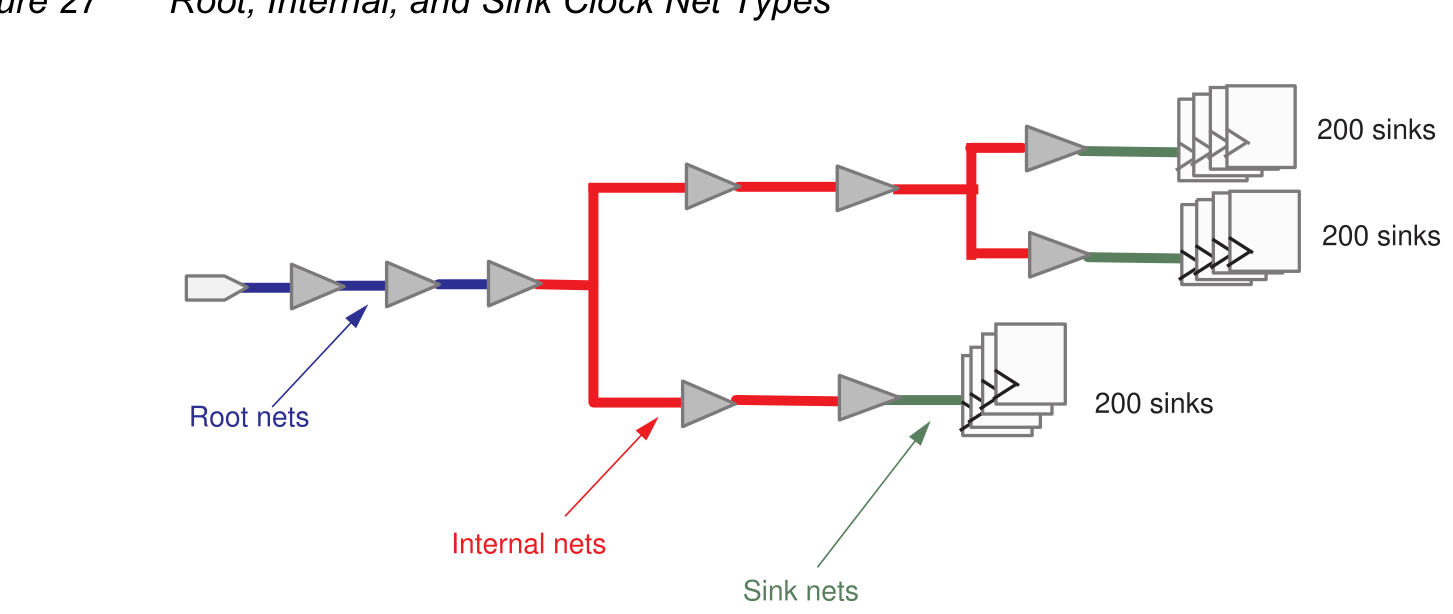
\includegraphics[width=0.92\textwidth,keepaspectratio]{figures/fig-ch2b-clock-net-types.png}
\caption{Root、Internal 与 Sink 时钟 Net 类型}
\label{fig:ch2b-clock-net-types}
\end{figure}

例如，布线 CLK1 的 root net 时使用 M4 至 M7：
\begin{lstlisting}
fc_shell> set_clock_routing_rules -clocks CLK1 -net_type root \
    -min_routing_layer M4 -max_routing_layer M7
\end{lstlisting}

识别 root net 时可用 \cmd{set\_clock\_tree\_options -root\_ndr\_fanout\_limit} 指定传递扇出上限。例如，传递扇出超过 300 个 sink 的时钟 net 视为 root net：
\begin{lstlisting}
fc_shell> set_clock_tree_options -root_ndr_fanout_limit 300
\end{lstlisting}

图~\ref{fig:ch2b-root-fanout} 示出指定传递扇出上限为 300 时同一时钟树的 root、internal 与 sink net。

\begin{figure}[htbp]
\centering
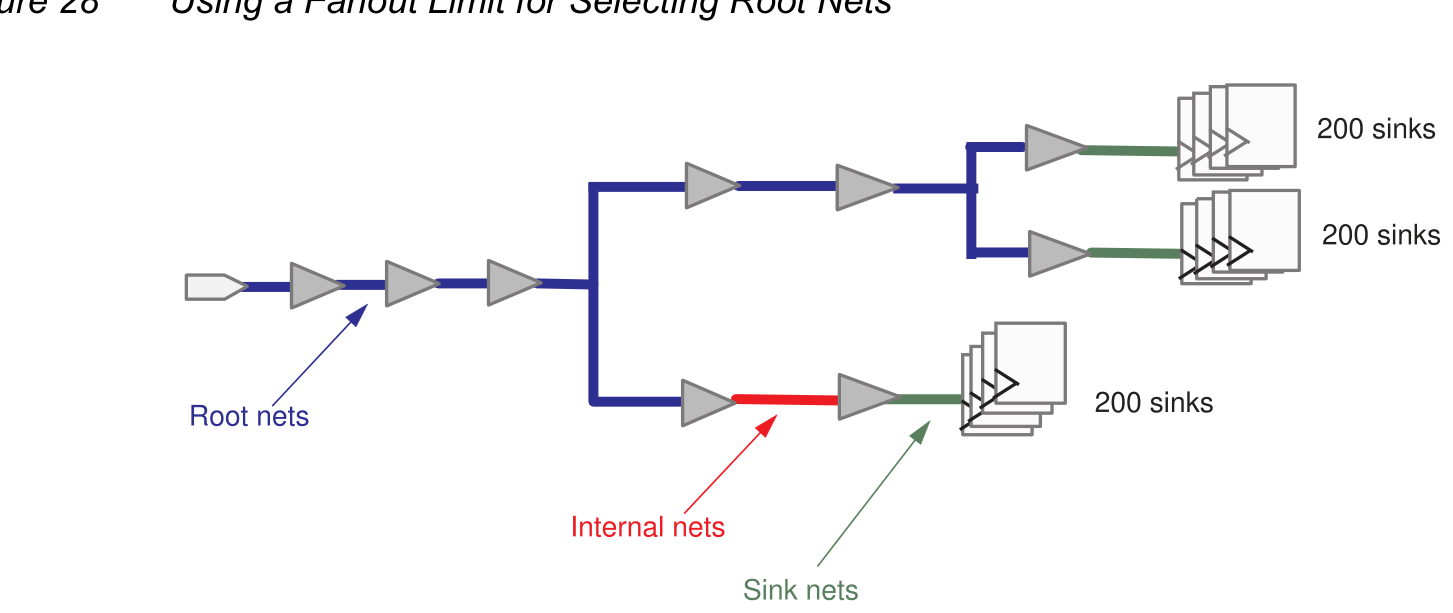
\includegraphics[width=0.92\textwidth,keepaspectratio]{figures/fig-ch2b-root-fanout.png}
\caption{用扇出限制选择 Root Net}
\label{fig:ch2b-root-fanout}
\end{figure}

计算传递扇出以识别 root net 时，工具仅计入有效时钟 sink，不包括 ignore pin。若被识别为 root 的 net 短于 10~micron，工具对该 net 使用 internal-net 层约束。

\begin{noteBox}
用较小的 \cmd{set\_clock\_tree\_options -root\_ndr\_fanout\_limit} 值会增加被赋 root-net 层约束的时钟 net 数量，可能加剧布线拥塞。
\end{noteBox}

移除该传递扇出限制，使用 \cmd{remove\_clock\_tree\_options -root\_ndr\_fanout\_limit}。

\subsection{启用基于 Level 的时钟非默认布线规则}
\subsubsection*{Enabling Level-Based Clock Nondefault Routing Rule}

时钟树综合期间，可按时钟树不同 level 为 net 分配连续的非默认布线规则。工具仅在初始 CTS 时实施变更，并按下列方式分配 NDR：
\begin{itemize}
  \item 仅连接到纯 sink 的 net：sink NDR
  \item 同时连接到 sink 与中间单元（repeater 或时钟门）的 net：internal NDR
  \item 从 root 级直至下游分支点的 net：root NDR
\end{itemize}

\begin{figure}[htbp]
\centering
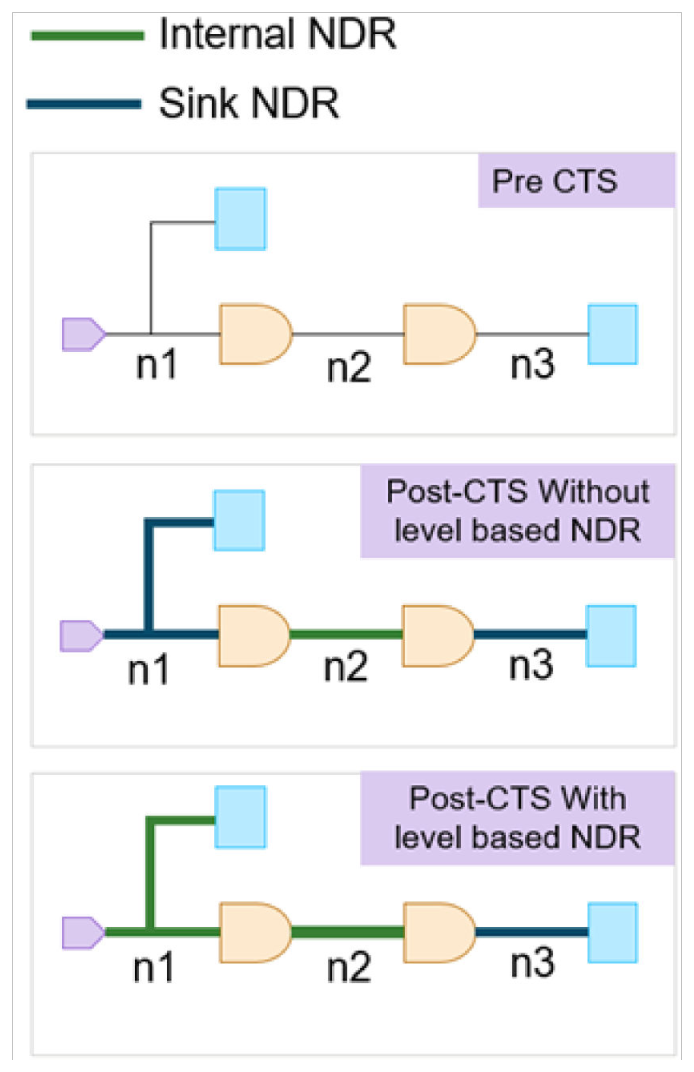
\includegraphics[width=0.50\textwidth,keepaspectratio]{figures/fig-ch2b-level-ndr.png}
\caption{基于 Level 的时钟非默认布线规则}
\label{fig:ch2b-level-ndr}
\end{figure}

如图所示，CTS 后：
\begin{itemize}
  \item \textbf{未启用}基于 level 的时钟 NDR：\texttt{n1} 与 \texttt{n3} 因至少连接一个 sink，编译时钟树后须获得 sink NDR；这会使不同 level 上出现不连续的 NDR。
  \item \textbf{启用}基于 level 的时钟 NDR：时钟树路径上全部 NDR 须按拓扑从时钟 root 到 sink 排序，即 Root NDR $>$ Internal NDR $>$ Sink NDR。因此 \texttt{n1}、\texttt{n2} 赋 internal NDR，\texttt{n3} 赋 sink NDR。
\end{itemize}

启用该功能：
\begin{lstlisting}
fc_shell> set_app_options -list {cts.compile.topological_ndr true}
\end{lstlisting}

\subsection{为层设置优选布线方向}
\subsubsection*{Setting the Preferred Routing Direction for Layers}

Fusion Compiler 要求为工艺文件中定义的布线层指定优选布线方向。通常该信息在单元库中定义。要设置或更改某层的优选布线方向，按下列语法设置其 \texttt{routing\_direction} 属性：
\begin{lstlisting}
set_attribute -objects layers
   -name routing_direction
   -value vertical | horizontal
\end{lstlisting}

用工艺文件中的层名指定布线层。该属性设置的层方向仅作用于当前 block。

例如，将 M5 与 M7 的优选方向设为 vertical：
\begin{lstlisting}
fc_shell> set_attribute -objects [get_layers {M5 M7}] \
   -name routing_direction -value vertical
\end{lstlisting}

\begin{noteBox}
用 \cmd{create\_routing\_guide -switch\_preferred\_direction} 在 routing guide 覆盖区域内更改优选方向的设置，会覆盖 \texttt{routing\_direction} 属性设置。
\end{noteBox}

报告一个或多个布线层的用户定义优选方向，使用 \cmd{get\_attribute}；移除则使用 \cmd{remove\_attributes}。

\begin{seeAlsoBox}
准备布线层。
\end{seeAlsoBox}

% ============================================================
\section{使用 Early Data Check Manager 处理设计数据}
\subsection*{Handling Design Data Using the Early Data Check Manager}

设计周期早期迭代中，设计数据可能不完整或不正确，从而妨碍探索性实现等。Fusion Compiler Early Data Check Manager 允许指定工具在下列实现任务中如何处理数据检查：
\begin{itemize}
  \item 设计规划
  \item 多电压设计实现
  \item 优化
  \item 布局
  \item 合法化
  \item 含物理层次设计的层次化实现
\end{itemize}

下表列出用于控制数据检查处理方式及生成相关信息的 Early Data Check Manager 命令。

\begin{table}[htbp]
\centering
\caption{Early Data Check Manager 命令（原书 Table 15）}
\label{tab:ch2b-edc}
\begin{tabularx}{\textwidth}{@{}X l@{}}
\toprule
\textbf{目的} & \textbf{使用的命令} \\
\midrule
指定一个或多个数据检查的处理策略 & \cmd{set\_early\_data\_check\_policy} \\
获取数据检查违例报告 & \cmd{report\_early\_data\_checks} \\
获取可在其他命令中使用的违例 Tcl 集合 & \cmd{get\_early\_data\_check\_records} \\
将设置保存到文件供日后使用 & \cmd{write\_early\_data\_check\_config} \\
清除数据检查设置以便下一轮迭代 & \cmd{remove\_early\_data\_check\_records} \\
\bottomrule
\end{tabularx}
\end{table}

应在开始实现前指定数据检查处理策略。

下列示例指定对 SCANDEF 信息检查采用严格策略，因此因缺少 SCANDEF，工具不会继续执行 \cmd{create\_placement}：
\begin{lstlisting}
fc_shell> set_early_data_check_policy -policy strict \
   -check place.coarse.missing_scan_def
fc_shell> create_placement
Information: Policy for early data check 'place.coarse.missing_scan_def'
 is 'error'. (EDC-001)
Error: No valid scan def found. (PLACE-042)
Information: Ending 'create_placement' (FLW-8001)
fc_shell> report_early_data_checks -check place.coarse.missing_scan_def
Check                           Policy Strategy Fail Count
-------------------------------------------------------------
place.coarse.missing_scan_def   error             1
-------------------------------------------------------------
\end{lstlisting}

下列示例对所有与粗布局相关的数据检查采用宽松策略，因此即使无 SCANDEF，工具仍继续 \cmd{create\_placement}：
\begin{lstlisting}
fc_shell> set_early_data_check_policy -policy lenient \
    -check place.coarse.*
fc_shell> create_placement
Information: Policy for early data check 'place.coarse.missing_scan_def'
 is 'tolerate'. (EDC-001)
Continuing without valid scan def.
Start transferring placement data.
Creating placement from scratch.
...
\end{lstlisting}

更多信息见 \textit{Fusion Compiler Data Model User Guide}。

% ============================================================
\section{应用 Mega-Switch 命令设置}
\subsection*{Applying Mega-Switch Command Settings}

可用 mega-switch 命令，以单一命令为工具流程不同阶段应用适用于特定情形的设置：
\begin{itemize}
  \item 应用先进工艺节点所需设置
  \item 应用高性能核所需设置
  \item 应用改善特定 QoR 指标所需设置
\end{itemize}

\subsection{应用先进工艺节点所需设置}
\subsubsection*{Applying Required Settings for Advanced Technology Nodes}

要对 12~nm 或 7~nm 工艺节点应用特定于布局、合法化、布线与提取的设置，使用 \cmd{set\_technology} 的 \opt{-node 12} 或 \opt{-node 7}。

使用该命令时，在布局、优化与布线前执行：
\begin{enumerate}
  \item 加载并 link 设计。
  \item 用 \cmd{set\_technology -node} 应用工艺节点所需设置，例如：
\begin{lstlisting}
fc_shell> set_technology -node 7
\end{lstlisting}
  \item （可选）用 \cmd{set\_technology -report\_only} 报告工艺节点设置。
  \item 应用设计专用应用选项或命令设置，以覆盖 \cmd{set\_technology} 的通用设置。
\end{enumerate}

用 \cmd{save\_lib} 保存设计库时，工艺节点设置一并保存。

\begin{noteBox}
用 \cmd{set\_technology} 指定工艺节点后，不可再更改。
\end{noteBox}

该命令支持哪些 ASIC 工艺，请联系 Synopsys Support。

\subsection{应用高性能核所需设置}
\subsubsection*{Applying Required Settings for High Performance Cores}

可用 \cmd{set\_hpc\_options} 应用为实现高性能核最佳 QoR 所需的工具设置。所应用设置影响布局、合法化、优化、时钟树综合、布线、提取与时序分析。

\begin{itemize}
  \item 列出支持的高性能核类型与实现阶段：用 \opt{-list}
  \item 指定高性能核类型：用 \opt{-core}
  \item 指定实现流程阶段：用 \opt{-stage}
\end{itemize}

若设计使用 12~nm 或 7~nm 节点，须在运行 \cmd{set\_hpc\_options} 前先用 \cmd{set\_technology} 应用节点专用设置，示例如下：
\begin{lstlisting}
set_technology -node 7
set_hpc_options -core A72 -stage clock_opt_cts
...
clock_opt -from build_clock -to route_clock
...
set_hpc_options -core A72 -stage clock_opt_opto
...
clock_opt -from final_opto
...
set_hpc_options -core A72 -stage route_auto
...
route_auto
...
set_hpc_options -core A72 -stage route_opt
...
route_opt
...
\end{lstlisting}

\subsection{应用改善特定 QoR 指标所需设置}
\subsubsection*{Applying Required Settings for Improving Specific QoR Metrics}

要用 \cmd{set\_qor\_strategy -stage pnr} 应用改善特定 QoR 指标所需的工具设置。

用 \opt{-metric} 指定要改善的 QoR 指标。为获得最佳：
\begin{itemize}
  \item 时序：使用 \texttt{timing}
  \item 漏电功耗与时序：使用 \texttt{leakage\_power}
  \item 总功耗与时序：使用 \texttt{total\_power}。\\
        为进一步改善总功耗（以 runtime 为代价），可与 \opt{-metric total\_power} 联用 \opt{-mode extreme\_power}。
\end{itemize}

用 \opt{-mode} 指定设计流程目标模式。支持取值：
\begin{itemize}
  \item \texttt{balanced}：默认模式，针对 \opt{-metric} 指定的目标指标优化设计。
  \item \texttt{early\_design}：适用于设计流程早期、侧重短周转时间原型的阶段。\\
        该模式可以 QoR 为代价缩短 runtime。
  \item \texttt{extreme\_power}：建议用于以 runtime 为代价进一步改善总功耗。\\
        仅应与 \opt{-metric leakage\_power} 或 \opt{-metric total\_power} 联用。若与 \opt{-metric timing} 联用，工具忽略该 mode 并使用 \texttt{balanced}。
\end{itemize}

使用该命令时，工具应用影响优化、布局、合法化、时钟树综合、布线、提取与时序分析的应用选项设置。

查看所需设置可用：
\begin{itemize}
  \item 用 \opt{-output} 生成包含这些设置的 Tcl 脚本
  \item 用 \opt{-report\_only} 报告设置
  \item 用 \opt{-diff\_only} 仅报告未设为所需值的设置
\end{itemize}

% ===== 第 2 章结束（原书约 p.180）=====
